\documentclass[12pt, a4paper, oneside, oldfontcommands, dvipsnames]{memoir}
\chapterstyle{veelo}
\copypagestyle{fancyheads}{companion}
\makeevenhead{fancyheads}{\thepage}{}{\sffamily\leftmark}
\makeoddhead{fancyheads}{\sffamily\rightmark}{}{\thepage}

%% TOC Depth
\setsecnumdepth{subsection}
\maxsecnumdepth{subsection}
\settocdepth{subsubsection}
\maxtocdepth{subsubsection}

%-----------------------------------------------------------------------------%
% Packages
%-----------------------------------------------------------------------------%

%% Graphics
\usepackage{pdfpages}
\usepackage{subcaption}
\usepackage{wrapfig}
\usepackage{graphicx}
\usepackage{epstopdf}
\graphicspath{ {img/} }
\usepackage{pgfplots}
\usepackage{pgfplotstable}
\pgfplotsset{%
    every linear axis/.append style={
        bar width=13pt,%
        major x tick style = transparent%
    }
}
\pgfplotsset{compat=1.8}
\usepgfplotslibrary{statistics}
\definecolor{LightGray}{RGB}{120,120,120}
\definecolor{VeryLightGray}{RGB}{247,247,247}
% \definecolor{DarkGray}{RGB}{39,40,34}
\definecolor{DarkGray}{RGB}{0,0,0}
\definecolor{MonokayBg}{RGB}{39,40,34}
\definecolor{Tufte}{rgb}{0.7,0.7,0.55}
\usepackage{tikz}
\usetikzlibrary{pgfplots.groupplots}
\usetikzlibrary{positioning,calc,shapes}
\tikzstyle{every picture}+=[font=\sffamily]
\tikzset{%
  component/.style={%
    text=white, fill=LightGray, text width=10em,
    minimum height=2em, text centered
  },
  arrow/.style={thick,->,shorten >=2pt,shorten <=2pt,>=stealth},
  number/.style={circle,fill=black, text=white, font=\tiny\bfseries, inner sep=0pt, minimum height=1em, anchor=base, text centered},
  dbscan/.style={%
    shape=circle,draw, minimum size=25mm
  },
  dbscan_circle/.style={%
    fill=black,minimum size=.5mm
  },
  class/.style={%
    draw,
    shape=rectangle split,
    rectangle split parts=3,
    font=\ttfamily,
    text width=6cm,
    rectangle split part align={center,left,left},
    rectangle split part fill={black, white, white},
    every text node part/.style={white, font=\sffamily, align=center}
    },
  process/.style={%
  },
  example/.style={%
    shape=rectangle split,
    rectangle split parts=2,
    font=\rmfamily,
    text width=.98\textwidth,
    rectangle split part align={center,left},
    rectangle split part fill={DarkGray, VeryLightGray},
    every text node part/.style={white, font=\sffamily, align=left}
    },
}
\usepackage{sansmath}

%% Math
\usepackage{amsmath}
\usepackage{amssymb}
\usepackage{mathtools}
\usepackage{abraces}

%% Typesetting
\usepackage{ragged2e}
\hyphenation{da-ta-base}
\usepackage{marginnote}
\usepackage{pgfplotstable}
\usepackage{calc}
\usepackage{blindtext}
\usepackage{metalogo}
\usepackage[htt]{hyphenat}
\usepackage{lettrine}
\usepackage{booktabs}
\usepackage{multirow}
\usepackage{xcolor,colortbl}
\newcolumntype{a}{>{\columncolor{LightGray!30}}c}
\usepackage{xspace}
\usepackage{url}
\usepackage{acronym}
\usepackage{fontspec}
\setmainfont[Ligatures=TeX]{Minion Pro}
\setsansfont{Myriad Pro}
% \newfontfamily\authorfont{Edwardian Script ITC}
\newfontfamily\authorfont{Zapfino}
\setmonofont[Scale=MatchLowercase]{Monaco}
\newfontfamily\HeadingsFont{Myriad Pro}
\newfontfamily\CaptionsFont{Myriad Pro}
\usepackage{titlesec}
\newcommand{\titlebar}{
    \tikz[baseline,trim left=3.1cm,trim right=3cm] {
        \node [anchor=base east,
               minimum height=3.5ex,
               fill=DarkGray,
               text=white] at (3cm,0) {\thesection};
    }
}
\titleformat{\section}{\large\bfseries\HeadingsFont}{\titlebar}{0.1cm}{}
\usepackage{caption}
\DeclareCaptionFont{white}{\color{white}}
\DeclareCaptionFormat{figure}{
  \colorbox{DarkGray}{%%%%
     \parbox{\dimexpr\columnwidth-2\fboxsep}{\hspace{.1cm}#1#2#3}%
  }
}
\captionsetup{format=figure,
                      labelfont=white,
                      textfont=white,
                      margin=0pt,
                      font={bf,small,sf}}
\usepackage{enumitem}
\SetLabelAlign{parright}{\parbox[t]{\labelwidth}{\raggedleft#1}}
\setdescription{leftmargin=1.4\parindent,labelindent=\parindent}
\usepackage{newverbs}
\newverbcommand{\bverb}
  {\begin{lrbox}{\verbbox}}
  {\end{lrbox}\colorbox{gray!30}{\box\verbbox}}

%% Code Listings
\usepackage{verbments}
\plset{%
    listingnamefont=\sffamily\bfseries\color{white},%
    captionfont=\sffamily\color{white},captionbgcolor=DarkGray,%
    numbers=left,
    style=tango,
    fontsize=\footnotesize,
    fvset={frame=bottomline,
           framerule=1pt,
           rulecolor=\color{DarkGray},stepnumber=3}}
\usepackage{adjustbox}
\usepackage{verbatim}
\definecolor{shadecolor}{rgb}{.9, .9, .9}
\newenvironment{code}%
   {\par\noindent\adjustbox{margin=1ex,bgcolor=shadecolor,margin=0ex \medskipamount}\bgroup\varwidth\linewidth\verbatim}%
   {\endverbatim\endvarwidth\egroup}

%% Bibliography
\usepackage[numbers]{natbib}

%% References
\PassOptionsToPackage{hyphens}{url}
\usepackage{hyperref}
\hypersetup{%
  pdftitle={Cerberus: Detection and Characterization of Automatically-Generated Malicious Domains},
  pdfauthor={Edoardo Giovanni Colombo},
}
\usepackage{memhfixc}

%-----------------------------------------------------------------------------%
% New Commands
%-----------------------------------------------------------------------------%
\newcommand{\thesystem}{\textsc{Cerberus}\xspace}
\newcommand{\phoenix}{\textsc{Phoe\-nix}\xspace}
\newcommand{\start}[2]{\lettrine[lines=4]{\color{BrickRed}#1}{#2}}
\newcommand{\sectionstart}[2]{\lettrine[lines=2]{#1}{#2}}
\newcommand{\component}[1]{\textsc{#1}}
\newcommand{\important}[1]{\textbf{#1}}
\newcommand{\n}[1]{\tikz[baseline=(X.base)] \node[number] (X) {\sffamily #1};}
\renewcommand{\vec}[1]{\mathbf{#1}}
\newcommand{\dbnode}[4]{%
            \node[shape=circle,draw, minimum size=25mm] at (#1,#2)
            (#3) {\tikz \node[fill=black,minimum size=.5mm] (#4){}; };%
}
\newcommand*{\GoldenRatio}{1.61803398875}%
\newcommand*\mean[1]{\overline{#1}}
\newcommand{\dataexample}[1]{
\begin{center}
\begin{tikzpicture}
\node [example] {
            \nodepart{text} \textbf{A Sneak Peek at the Data.}
            \nodepart{two} \begin{minipage}{\textwidth-\parindent}%
            \vspace{.1cm}
            #1
            \end{minipage}};
\end{tikzpicture}
\end{center}}
\newcommand{\authorcol}[1]{{\tiny\authorfont #1}}

%-----------------------------------------------------------------------------%
% Meta Informations
%-----------------------------------------------------------------------------%
\author{}
\date{}
\title{\thesystem}

%-----------------------------------------------------------------------------%
% Language
%-----------------------------------------------------------------------------%
\usepackage[italian,english]{babel}
\selectlanguage{english}

%-----------------------------------------------------------------------------%
% Document Start
%-----------------------------------------------------------------------------%
\begin{document}
  \includepdf[pages={1}]{cover.pdf}
  \pagestyle{fancyheads}
    %-------------------------------------------------------------------------%
    % Title
    %-------------------------------------------------------------------------%
    \frontmatter
    \maketitle
    \clearpage
    \vspace*{8em}
      \begin{minipage}[t]{.55\textwidth}
      \begin{flushright}
            {\Large \textsf{Colophon}}

            \vspace*{1em}

            Typeset in \textsf{\XeTeX}\\
            by the \authorcol{Non-Roman}\\
            \authorcol{Script Initiative} \\
            and the \textsf{memoir} class\\
            created by \authorcol{Peter Wilson}~.\\
            The body text is set 12pt\\
            with Minion Pro. \\
            Other fonts include\\
             \texttt{Monaco} and \textsf{Myriad Pro}.\\
            Drawings typeset in\\
            \textsf{TikZ/PGF} packages\\
            by \authorcol{Till Tantau}~.

            \vspace*{2em}

            {\sffamily Pictures Credits}

            \vspace*{.5em}

            \textsf{Folder} designed by Eden Clairicia\\
            \textsf{Magnifying Glass} designed by Fusi Gabriele\\
            \textsf{Funnel} designed by Alberto Galindo\\
            \textsf{Delete} designed by P.J. Onori\\
            \textsf{Smartphone} designed by Martin Jordan\\
            \textsf{Hosting} designed by Tim Duppen\\
            \textsf{Pirate} designed by Simon Child\\
            \textsf{Computer} designed by Alex Valdivia\\
            \textsf{Laptop} designed by Olivier Guin\\

            \vspace*{.7em}

            All pictures were downloaded from\\
            \url{thenounproject.com}
            \end{flushright}
      \end{minipage}%
      \hspace{.1\textwidth}%
      \begin{minipage}[t]{.35\textwidth}
            \begin{flushleft}
                  {\Large \textsf{Research Places}}

                  \vspace*{1em}

                  
\includegraphics[width=.85\textwidth]{logo_polimi}

                  \vspace{1em}

                  
\includegraphics[width=.85\textwidth]{logo_necst.eps}

                  \vspace{1em}

                  
\includegraphics[width=.85\textwidth]{logo_rhul}

                  \vspace*{2em}

                  {\sffamily Proudly Written by}

                  \vspace{.8em}

                  
\includegraphics[width=3.5cm]{edo}

                  \vspace{.5em}

                  \authorcol{Edoardo Colombo}

            \end{flushleft}
            \begin{center}
            \end{center}

      \end{minipage}
    \vfill

    \thispagestyle{empty}
    \null\vspace{\stretch {1}}
        \begin{flushright}
            To \emph{Etta} and \emph{Nino}.
        \end{flushright}
\vspace{\stretch{2}}\null
    %!TEX root = ../thesis_polimi.tex


\chapter*{Abstract}
\start{B}{otnets}  are networks of infected machines (the \emph{bots}) controlled
by an external entity, the \emph{botmaster}, who uses this infrastructure to
carry out malicious activities, e.g., spamming and Distributed Denial of Service. The Command and Control Server (C\&C) is the machine
employed by the botmaster to dispatch orders to and gather data from the bots,
and the communication is established through a variety of distributed or
centralized protocols, which can vary from botnet to botnet. In the case of
DGA-based botnets, a Domain Generation Algorithm (DGA) is used to find the
\emph{rendezvous} point between the \emph{bots} and the \emph{botmaster}.
Botnets represent one of the most widespread and dangerous threats on the Internet and
therefore it is natural that researchers from both the industry and the academia
are striving to mitigate this phenomenon. The mitigation of a botnet
is a topic widely covered in literature, where we find many works that propose approaches
for its detection. Still, all of these systems suffer from the major
shortcomings of either using a supervised approach, which means that the system
needs some \emph{a priori} knowledge, or leveraging DNS data containing
information on the infected machines, which leads to issues related to the
users' privacy and the deployment of such systems.

We propose \thesystem, an automated system based on machine learning, capable to automatically discover new botnets and use this
knowledge to detect and characterize malicious activities. \thesystem analyzes passive
DNS data, free of any privacy issues, which allows the system to be easily
deployable, and uses an unsupervised approach, i.e., \thesystem needs no
\emph{a priori} knowledge. In fact the system applies a series of filters to
discard legitimate domains while keeping domains generated by AGDs and likely to be malicious. Then, \thesystem
keeps record of the activity related to the IP addresses of those domains, and,
after $\Delta$ time, it is able to isolate clusters of domains belonging to the same
malicious activity. This knowledge is later used to train a classifier that will analyze
new DNS data for detection.

We tested our system in the wild by analyzing one week of real passive DNS data.
\thesystem was able to detect 47 new clusters of malicious activities: Well
known botnets as \texttt{Jadtre}, \texttt{Sality} and \texttt{Palevo} were found among the others.
Moreover the tests we ran on the classifier showed an overall accuracy of 93\%, proving
the effectiveness of the system.


\selectlanguage{italian}
\chapter*{Ampio Estratto}
\start{L}{e botnet} sono considerate una tra le più diffuse minacce nell'Internet.
Analisti dal mondo dell'industria e ricercatori di sicurezza informatica sono
continuamente all'opera, al fine di mitigare questo fenomeno in perenne crescita.
Recenti rapporti redatti da McAfee~\cite{mcafee2013} ed Enisa~\cite{enisa2013}
confermano come tutte le attività malevoli presenti nell'Internet non mostrino il
minimo segno di scostamento dal loro continuativo tasso di crescita, botnet comprese.
Gli \emph{attacker} inoltre, colpiscono sempre più tipologie di piattaforme:
nell'aprile 2012 più di 600,000 computer Apple~\cite{enisa2012} furono infettati
dal \emph{malware} conosciuto come \texttt{Flashback}.
Inoltre, le minacce riguardanti piattaforme mobili, hanno visto un'impressionante
crescita, diventando un serio problema per gli utilizzatori di \emph{smartphone}
Android, il sistema operativo più colpito.

Una ricerca condotta da \citet{grier2012manufacturing} ha mostrato come
le attività malevole non siano più perpetrate dagli attaccanti a scopo ludico, ma
per fini lucrativi. Il sorgere del modello \emph{exploit-as-a-service} per
portare a compimento la compromissione del \emph{browser} tramite attacco
\emph{drive-by-download} è un fenomeno preoccupante, in cui i kit di exploit sono
venduti al pari di un qualsiasi altro prodotto per le necessità degli attaccanti.

Le stesse botnet sono ormai infrastrutture concepite esplicitamente per fini di lucro.
\texttt{Torpig} e \texttt{Zeus} ad esempio, mirano a rubare credenziali di accesso
a conti corrente dalle macchine infette e inviarli agli attaccanti. Un altro
tipo di malware lucrativo prende il nome di \emph{ransomware}.
Il \emph{ransomware} non è una nuova minaccia, tuttavia è tornata prepotentemente
in scena con l'avvento di \texttt{Cryptolocker}, un \emph{malware} capace di
collezionare guadagni che sono stati conservativamente stimati pari a
1,100,000 USD~\cite{spagnuolo2013}.

La mitigazione delle \emph{botnet} è pertanto di interesse primario per i \emph{difensori}, i quali a tale scopo concentrano i loro sforzi nell'individuare gli indirizzi
IP dei cosiddetti Server di Comando e Controllo (C\&C). Un Server C\&C è la
macchina dalla quale gli attaccanti inviano gli ordini e raccolgono i dati
provenienti dalle macchine infette. In un'architettura di botnet di tipo
centralizzato (la più diffusa), nel momento in cui la comunicazione tra il Server
C\&C e le macchine infette, i \emph{bots}, è terminata, questi ultimi diventano
\emph{dormienti} e solitamente innocui.

Gli attaccanti sono consci di questa debolezza nella loro infrastruttura, e hanno
sviluppato tecniche sempre più sofisticate al fine di rendere l'interruzione del
canale di comunicazione C\&C uno sforzo considerevole per i difensori.
A tale scopo, la maggior parte della comunicazione delle moderne botnet,
si appoggia sull'utilizzo dei Domain Generation Algorithm (DGA), che rendono
il punto di \emph{rendezvous} non prevedibile e il canale di comunicazione resistente
alle interruzioni. Questi algoritmi generano liste di domini casuali ogni $\Delta$
tempo, ad esempio un giorno, a volte utilizzando semi imprevedibili, domini che i \emph{bot}
tentano di contattare tramite richieste di tipo HTTP. L'attaccante registra solo un dominio e aspetta che uno dei \emph{bot} contatti l'URL corretto. Quando ciò accade,
la comunicazione ha inizio e i dati possono essere trasmessi in entrambe le direzioni.

La mitigazione delle botnet è un argomento ampiamente discusso in letteratura,
in cui vari autori hanno proposto strumenti di individuazione i quali, seppur
efficaci, si appoggiano principalmente su un approccio di tipo \emph{supervisionato}
o sugli indirizzi IP degli utenti o su entrambi: due aspetti che consideriamo come
difetti. Infatti, l'approccio supervisionato richiede che vengano forniti
dati etichettati in ingresso al sistema. Ciò comporta la necessità di avere un altro
modo per individuare la minaccia ed etichettarla, prima che il sistema possa essere
operativo. Inoltre questo approccio risulta minacciato da attività malevole che
mostrano caratteristiche prima non considerate. Utilizzare l'indirizzo IP degli
utenti è considerato un difetto poiché comporta problemi relativi alla privacy
degli utenti stessi e al dislocamento di un sistema di monitoraggio a livelli bassi
della gerarchia DNS.

Nel 2013, \citet{schiavoni2013} proposero \phoenix, un sistema di rivelazione che
soddisfa la maggior parte dei nostri criteri, poiché non richiede conoscenza
\emph{a priori} e analizza dati DNS passivi, franchi di qualsiasi problema legato
alla privacy. \phoenix è in grado di \emph{scoprire} cluster di domini utilizzati
per la comunicazione dei Server C\&C, svelando in tal modo i loro indirizzi IP,
e di \emph{individuare} domini malevoli, utilizzando la conoscenza prodotta
precedentemente. Nonostante i notevoli risultati, \phoenix non è in grado di
individuare \emph{i)} minacce che utilizzano Server C\&C con IP prima non visti,
\emph{ii)} minacce che modificano leggermente il DGA, e.g., cambiando l'insieme di
TLD utilizzati e \emph{iii)} manca di validazione con dati reali.

Noi proponiamo \thesystem, un sistema di individuazione che migliora i risultati
raggiunti da \phoenix, dimostrandosi capace di individuare minacce non note
utilizzando un approccio di tipo non supervisionato.

\thesystem affronta tre fasi per raggiungere questo risultato. La prima fase
prende il nome di \important{Fase di Bootstrap}, in cui utilizza \phoenix
per generare \emph{ground truth} da utilizzarsi in seguito durante la
\important{Fase di Detection}. La \emph{ground truth} è composta da una lista di
\emph{cluster} di domini che fanno riferimento ad attività malevole basate su DGA,
e.g., \emph{botnet} e \emph{trojan}.

Dopo che il sistema è stato inizializzato, comincia ad analizzare
un flusso di dati DNS passivi, il quale consiste di risposte DNS: il nome di dominio,
l'indirizzo IP a cui risolve e il TTL. Questi dati devono essere filtrati dai domini
legittimi. A tale scopo, durante la \important{Fase di Filtering}, una serie di
euristiche viene applicata ai dati, euristiche che tengono conto di parametri come
la data di registrazione il TLD utilizzato e il TTL. I domini che rimangono alla
fine del processo di filtraggio sono da considerarsi ``probabilmente malevoli''.

Questi domini sono i dati di ingresso per la sovracitata \important{Fase di Detection}, in cui proviamo a classificare tali dati utilizzando la conoscenza prodotta in
\important{Fase di Bootstrap}. A tale scopo, \thesystem guarda se il dominio
sconosciuto $d$ condivide il proprio indirizzo IP con uno dei cluster: in tal caso
alleniamo una Support Vector Machine equipaggiata con la funzione
Subsequence String Kernel~\cite{lodhi2002}, e la utilizziamo per classificare $d$.
Altrimenti iniziamo a registrare le attività legate all'indirizzo IP di $d$, $l$.
Ciò significa che teniamo traccia dei domini probabilmente malevoli che hanno
risolto su $l$ nel corso del tempo. Dopo una settimana di registrazione, \thesystem
raggruppa questi indirizzi IP sospetti a seconda dell'Autonomous System a cui
appartengono ed esegue una routine di clustering basata sull'algoritmo DBSCAN e
il Subsequence String Kernel come misura di distanza. Questi cluster sono poi
aggiunti alla \emph{ground truth} e la conoscenza ora aumentata viene utilizzata
per analizzare nuovi dati DNS.

Abbiamo eseguito un esperimento utilizzando dati passivi DNS reali,
raccolti da una macchina ISC/SIE nell'arco di una settimana. In questo periodo, \thesystem ha
classificato 187 domini malevoli, di cui 167 appartenevano alla minaccia chiamata
\texttt{Conficker}, precedentemente scoperta da \phoenix. Dopo sette giorni
avevamo raccolto 1,300 indirizzi IP sospetti, per un totale di 3,576 domini.
Quindi la routine di clustering è stata in grado di produrre 47 nuovi cluster,
i quali esibivano indirizzi IP noti, appartenenti a minacce come \texttt{Palevo}
e \texttt{Sality}. I cluster sono stati aggiunti alla precedente conoscenza e il
giorno seguente \thesystem è stato in grado di individuare 319 domini
malevoli.

\paragraph{Organizzazione del Documento}
Il resto del documento è organizzato nel modo seguente:
\begin{itemize}
    \item nel Capitolo~\ref{chap:botnets} forniremo le informazioni necessarie a comprendere il problema in analisi;
    \item nel Capitolo~\ref{chap:motivation} approfondiremo le motivazioni per cui
        abbiamo interesse a studiare questo fenomeno;
    \item nel Capitolo~\ref{chap:approach} presenteremo \thesystem, un
        sistema di rivelazione di attività malevole basate su DGA;
    \item nel Capitolo~\ref{chap:implementation} spiegheremo come \thesystem
        è stato implementato e le tecnologie impiegate;
    \item nel Capitolo~\ref{chap:validation} verificheremo l'efficacia di
    \thesystem;
    \item nel Capitolo~\ref{chap:conclusions} analizzeremo i difetti di
    \thesystem e proporremo alcuni possibili rimedi, assieme a sviluppi futuri.
\end{itemize}

\selectlanguage{english}

    \chapter*{Acknowledgements}

\start{M}{y first}  thank you goes to my parents,
Laura and Carlo, who have always encouraged me to follow my
dreams and my passions. They have supported me during my whole life, especially during these five years at the Politecnico: They have always decided to sacrifice something of theirs to make my life better. Among other things, I would like to especially thank them
as they allowed me to study at the
University of Illinois at Chicago, one of the greatest
experiences of my life.\\
I love you.

\vspace{1cm}

I would like to thank Prof. Stefano Zanero, Prof. Lorenzo Cavallaro and Prof.
Federico Maggi
for helping me throughout my research efforts. They are the most professional
and passionate professors and researchers I have ever met, and it was a true pleasure
to work together. A special thank you to Prof. Stefano Zanero who has allowed me
to go as a visiting student to the Royal Holloway University of London, and to
Prof. Lorenzo Cavallaro who hosted me and made me feel more than welcome.

\vspace{1cm}

I would also like to thank my friends, who have supported me, and the people at the
NECST Lab, where I spent endless hours working with them. It is a really nice
environment for research, where labor and fun are harmonically mixed.

\vspace{1cm}

\begin{flushright}
Once again, thank you to all of you.\\
\emph{I am what I am because of who we all are.}
\end{flushright}


    %-------------------------------------------------------------------------%
    % Tables
    %-------------------------------------------------------------------------%
    \tableofcontents
    \listoffigures
    \listoftables
    \listofpyglistings

    %-------------------------------------------------------------------------%
    % Chapters
    %-------------------------------------------------------------------------%
    \mainmatter
    %!TEX root = ../thesis_polimi.tex

\chapter{Introduction} % (fold)
\label{chap:introduction}

\start{B}{otnets} are one of the most widespread threats on the Internet. Analysts
from the industry and security researchers are both striving to mitigate such
ever increasing phenomenon. Recent reports from McAfee~\cite{mcafee2013} and
Enisa~\cite{enisa2013} confirm that all malicious activities on the Internet show
no disruption of their steady growth, botnets included.
Attackers are also widening the spectrum of targeted platforms: In April 2012
it was reported that more than 600,000 Apple computers~\cite{enisa2012} were infected
by the \texttt{Flashback} malware, which turned these machines into bots.
Moreover, mobile threats have experienced an
outstanding increase, becoming a serious problem for Android users, being
the mobile OS by Google the most targeted platform.

Also, research by \citet{grier2012manufacturing} illustrates how the malicious
activities are no longer perpetrated for no-profit reasons of miscreants'
entertainment, but do involve economical returns. Emergence of the
\emph{exploit-as-a-service} business model~\cite{grier2012manufacturing} is a worrying new phenomenon, where exploit kits are
sold likewise as a commodity for attackers' needs.

Botnets themselves are becoming infrastructures that are unashamedly crafted for
lucrative goals. \texttt{Torpig} and \texttt{Zeus} for instance aim at stealing
financial accounts credentials from the infected machines and send them back to the
attackers. Another lucrative kind of malware is \emph{ransomware}.
Ransomware is a not new, yet never as scary, threat that has made the news lately
with the coming of \texttt{Cryptolocker}, a malware able to collect revenues that
were \emph{conservatively} estimated at 1,100,000 USD~\cite{spagnuolo2013}.
The communication between the infected machines and the attacker, and the infection itself were realized by the means of a botnet.

Therefore the mitigation of botnets is of primary interest for defenders, and to
this end their efforts focus on unveiling the IP addresses of the so called
Command \& Control Servers (C\&C hereafter). A C\&C Server is the machine from
where the attackers dispatch their orders to and collect data from the infected
machines. In a centralized botnet architecture (the most prevalent), once the communication between
the C\&C and the infected machines, the \emph{bots}, is disrupted, the latter
become \emph{dormant} and usually harmless.

Attackers are well aware of the most precious asset and weakness in their
infrastructure and have developed increasingly sophisticated techniques to make
the disruption of the C\&C channel a fatiguing endeavor on the defenders' side. To this end, most of nowadays' centralized
botnets' communication relies on the employment of Domain Generation Algorithms
(DGAs hereafter), which make the \emph{rendezvous} point (i.e., the moment when the bot \emph{finds} the botmaster) unpredictable and the communication channel resilient to interruptions. These algorithms generate lists of random domains every $\tau$ time, say daily, sometimes employing unpredictable seeds, which the
bots try to contact. The attacker registers one domain and
awaits for the \emph{zombies} to reach the correct URL. When this happens the
communication can start and data can be transmitted in both directions.

The mitigation of botnets is a topic widely covered in literature, \cite{antonakakis2011} \cite{bailey2009} \cite{bilge2012}  \cite{neugschwandtner2011}
\cite{schiavoni2013} \cite{sharifnya2013} \cite{gross2009}, where many
authors
propose detection tools which, yet effective, mostly rely either on a \emph{
supervised} approach or on clients' IP addresses or on both, two aspects that
we deem as shortcomings. In fact, the supervised approach requires labeled data to
be fed to the system, which means that before the detection can be actually
started, there has to be another way to track the threat and label it as such. Moreover this approach
suffers from new menaces that exhibit features previously not considered, as a
change in the DGA.
Leveraging clients' IP addresses is a shortcoming as it leads to difficulties
related to the clients' privacy and the deployment of a monitoring system at lower
levels of the DNS hierarchy.

In 2013, \citet{schiavoni2013} proposed \phoenix, a detection system that meets
most of our criteria, as it does not require any \emph{a priori} knowledge and it
analyzes passive
DNS data, free of any privacy issues. \phoenix is able to \emph{discover}
clusters of domains used as aliases for botnets' C\&C servers, thus unveiling
their IP addresses, and to \emph{detect} malicious domains, using the knowledge
(i.e., the clusters) previously generated. Despite these valuable features,
\phoenix is not able to detect \emph{i)} threats that use C\&C servers with
previously unseen IP addresses, \emph{ii)} threats that dynamically slightly modify the
DGA, e.g., by changing the set of TLDs used and \emph{iii)} it lacks
of validation in the wild.

We propose \thesystem, a detection system that overcomes the aforementioned limitations of
\phoenix, being able to detect previously unseen threats in the wild using
an \emph{unsupervised} approach.
\thesystem goes through three stages to achieve its goals. The first phase is
called \important{Bootstrap Phase}, where it uses \phoenix to generate the
ground truth, later to be employed in the \important{Detection Phase}, in an
unsupervised and automatic fashion. The ground
truth consists of a list of clusters of domains related to DGA-based malicious
activities, e.g., botnets and trojans. This ground truth is not necessary to
\thesystem to function, as it is able to operate in a complete unsupervised fashion.

After the system has been bootstrapped, it starts analyzing a live
stream of DNS passive data, which consists of DNS replies: the domain name, the IP
address it resolves to and the TTL. This data needs to be filtered from legitimate
domains. To this end during the \important{Filtering Phase}, we apply a list of heuristics to the data, heuristics that take into account parameters as the
registration date, the TLD employed and the TTL. The domains that remain at the
end of the filtering process are to be considered likely to be malicious.

These domains are the input to the aforementioned \important{Detection Phase},
where we try to label this data using the ground truth generated in the
\important{Bootstrap Phase}. To this purpose, \thesystem sees whether the unseen
domain $d$ shares its IP address with the clusters: If this is the case we train
a Support Vector Machine equipped with the Subsequence String
Kernel~\cite{lodhi2002} function and we use it to label $d$. Otherwise, we start
keeping track of the IP of $d$, $l$. This means that we record the likely-to-be-
malicious domains that
resolve to $l$ throughout time. After $\Delta$ time of recording, \thesystem groups
these suspicious IPs by the Autonomous System that they reside in and performs a
clustering routine that leverages the DBSCAN algorithm and the Subsequence String
Kernel as a metric. These clusters are then added to the ground truth and the
increased knowledge is then used to analyze new live DNS data.

We used one week of real passive DNS data collected by a ISC/SIE
passive DNS monitor to test our system. During the first week \thesystem classified 187 malicious
domains, 167 of which belonged to the \texttt{Conficker} threat, previously
discovered by \phoenix. At the end of the week we had collected 1,300 suspicious
IP addresses, for a total of 3,576 domains. Then the clustering routine was able
to extract 47 new clusters, featuring known malicious IP addresses of
threats as \texttt{Palevo} and \texttt{Sality}. The clusters were added to the
previous knowledge and the day after \thesystem was able to detect 319 malicious
domains.

\paragraph{Document Organization}
The remainder of this document is organized in the following fashion:
\begin{itemize}
    \item Chapter~\ref{chap:botnets} provides the background knowledge
        needed to understand the phenomenon we aim at analyzing. We give
        a definition of what a botnet is in Section~\ref{sec:what_is_a_botnet}, why the attackers are interested in Section~\ref{sub:purposes} in setting up this type of infrastructure, how a botnet can be structured in Section~\ref{sec:botnet_topologies},
        the communication system between the botmaster and the bots in Section~\ref{sec:botnets_communications}, focusing on the Domain Generation Algorithms in Section~\ref{sec:domain_generation_algorithms} and the countermeasures that can be applied
        to mitigate this threat in Section~\ref{sec:botnet_countermeasures}. Then we
        present two case studies of botnets active in the wild, \texttt{Torpig}
        and \texttt{Cryptolocker} in Section~\ref{sec:botnets_a_modern_threat};
    \item Chapter~\ref{chap:motivation} discusses why we want to study
        this phenomenon, in Section~\ref{sec:state_of_the_art} we present
        the current the state of the art we wish to improve and
        in Section~\ref{sec:goals_and_challenges} the goals and challenges
        we mean to achieve and face, respectively;
    \item Chapter~\ref{chap:approach} introduces \thesystem, a
        detection system for DGA-based malicious activities. In Section~\ref{sec:approach_overview} we  give an overview of the system, while in
        Section~\ref{sec:approach_details} we  discuss in details all of
        its aspects;
    \item Chapter~\ref{chap:implementation} explains how \thesystem
        was implemented and the technologies employed, describing the overall
        architecture (see Section~\ref{sec:system_architecture})), the process in Section~\ref{sub:the_process} and then the actors involved in Section~\ref{sub:the_actors}
        during the system's lifecycle. Then we focus on the most crucial
        parts and provide a more detailed description of those in Section~\ref{sec:system_details};
    \item in Chapter~\ref{chap:validation} we test the effectiveness of our system.
        To this end we run two tests. The first one serves to confirm the
        accuracy of the SVM Classifier, and it employs the clusters generated
        by \phoenix as dataset. For the second one instead we use DNS passive
        data collected by a ISC/SIE DNS monitor. We let \thesystem analyze one
        week of data and look at the results, which look promising;
    \item Chapter~\ref{chap:conclusions} analyzes the shortcomings
        \thesystem is affected by and proposes possible remedies to them, along with a few possible enhancements and future developments. Finally,
        it sums up what we achieved in this work;
\end{itemize}
% chapter introduction (end)

    %!TEX root = ../thesis_polimi.tex

\chapter{Botnets} % (fold)
\label{chap:botnets}
\start{A}{botnet} is a network of compromised machines, remotely controlled
by the \emph{botmaster}. These malicious infrastructures are deployed by the
attackers for profit, and the more machines are compromised, the more powerful the
infrastructure, the more profitable the business. In the last years we
have witnessed an aggressive spread of this phenomenon that \emph{defenders}
from both the industry and the academia are striving to mitigate. In this
chapter we will tackle the different aspects of botnets in order to give
a brief yet insightful overview of this threat.

\paragraph{Chapter Organization} The remainder of the chapter is organized in
the following fashion:
\begin{itemize}
    \item in Section~\ref{sec:what_is_a_botnet} we explain what is a botnet;
    \item in Section~\ref{sec:botnet_topologies} we explain the different
        topologies a botnet can feature;
    \item in Section~\ref{sec:botnets_communications} we explain how botnet's
        hosts communicate;
    \item in Section~\ref{sec:domain_generation_algorithms} we deeper analyze
        a certain way to communicate, on which we focus in
        \thesystem;
    \item in Section~\ref{sec:botnet_countermeasures} we overview the possible
        techniques to mitigate a botnet;
    \item in Section~\ref{sec:botnets_a_modern_threat} we provide two case
        studies to better  explain why this phenomenon is a serious and expanding
        threat.
\end{itemize}


\newpage

%-----------------------------------------------------------------------------%
% Section: What is a botnet?
%-----------------------------------------------------------------------------%
\section{What is a botnet?} % (fold)
\label{sec:what_is_a_botnet}
\sectionstart{A}{botnet} is a network of compromised machines called \emph{bots}
or \emph{zombies} under the remote control of a human operator called
\emph{botmaster}~\cite{feily2009}.


The \emph{bot} is the piece of software that infects and compromises the machines.
The infection is carried out through a variety of so-called \emph{distribution channels}, which vary from compromised websites that serve malware via drive-by
mechanisms to phishing.
Once infected, the machine will continue to work as nothing changed to the eyes
of the legitimate user, while it is now capable of executing malicious
activities on the behalf of the \emph{botmaster}, who will employ a Command and
Control Server (C\&C) to dispatch orders to and gather information from
the \emph{zombies}. What is the nature of these criminal activities are
addressed in the next paragraphs.

\begin{figure}[!htp]
\centering
\begin{tikzpicture}[scale=0.6, every node/.style={transform shape}]
    \node [label=below:C\&C Server](CANDC) {
\includegraphics{server.eps}};
    \node [label=below:Botmaster](MASTER) [left=2cm of CANDC]{
\includegraphics{attacker.eps}};
    \node [label=below:Zombie](LAPTOP) [above right = 3cm of CANDC] {
\includegraphics{laptop_infected}};
    \node [label=below:Zombie](LAPTOP_2) [right = 3cm of CANDC] {
\includegraphics{nexus_infected.eps}};
    \node [label=below:Zombie](LAPTOP_3) [below right = 3cm of CANDC] {
\includegraphics{desktop_infected}};

    \path[arrow, <->]
        (CANDC) edge (LAPTOP)
        (CANDC) edge (LAPTOP_2)
        (CANDC) edge (LAPTOP_3);

    \path[arrow]
        (MASTER) edge (CANDC);
\end{tikzpicture}
\caption{An example of a botnet.}
\label{fig:botnet_example}
\end{figure}

\subsection{Botnet Purposes} % (fold)
\label{sub:purposes}
The main purpose of a malicious botmaster is to recruit as many \emph{zombies} as possible
in his army, as any botnet activity augments its effectiveness by the number
of \emph{bots} involved. In the following of this section we depict \emph{a few}
scenarios of malicious activities carried out employing this type of infrastructure.

\paragraph{Information Gathering} Botnets of this type aim at stealing personal
data of various kind from the infected machines. \texttt{Torpig} for instance,
which we shall further analyze in Section~\ref{sub:torpig}, was crafted with the precise
intention of stealing financial accounts credentials and credit or debit card
numbers. Beside personal data, we can think of a scenario where the infected
machines reside inside a corporate network. In this case the targets would be
trade secrets, as intellectual properties or management plans.

\paragraph{Distributed Computing} The network of infected machines can be
leveraged to perform computing-intensive tasks. One of the most interesting
ones is Bitcoin mining: Cybercriminals aim at creating a botnet of infected machines forced to perform complex calculations to earn them money, putting the
machines under heavy CPU and GPU load~\cite{spagnuolo2013}.
\texttt{Trojan.Coinbitminer} is an example of this type of
malware\footnote{\url{http://www.symantec.com/security_response/writeup.jsp?docid=2011-072002-1302-99}}.

\paragraph{Spamming} Spamming is one of the most known malicious activities.
Spamming botnets are used to send out a high volume of e-mails with various purposes, amongst which
we find malware spreading as an e-mail attachment (the \texttt{Cryptolocker} malicious binary was spread in this
fashion in its early versions, see Section~\ref{sub:cryptolocker}), frauds, XSS attacks and
advertisement of malicious services, basically using the bots as mail transfer agents without the victims noticing. It is not easy to set up and keep active
such an infrastructure, as spam sources get blacklisted and the messages are no
longer delivered. By employing a \emph{distributed} rather than \emph{centralized}
message dispatching servers architecture, the attackers aim at and succeed in
circumventing this obstacle.

\paragraph{Distribute Denial of Service} Distribute Denial of Service (DDoS)
is an attack where a machine receives an excessive amount of requests. To overcome
the overwhelming volume of incoming traffic, usually the machine interrupts its
services. This results in economic loss, especially when the company business
heavily depends on the offered service online availability. In this case the bots
are commanded by the botmaster to send an excessive amount of requests to the
targeted machine.

\paragraph{Malware Diffusion} Once the \emph{bot} program infects a machine,
it can be used to install \emph{further} malware. An example of this behavior
comes from the recent Cryptolocker \emph{ransomware}: Its primary vector of
infection was the \texttt{Zeus Gameover} P2P botnet, beside being spread via
e-mail spamming.
% subsection purposes (end)

\subsection*{Summary} % (fold)
\label{sub:what_summary}
In this section we have defined \emph{what} is a botnet and discussed \emph{why}
an attacker would struggle to create this type of networks. In the next section
we want to present the different topologies a botnet can be structured into and
explain why we chose to target the \emph{centralized} architecture.

% subsection summary (end)
% section what_is_a_botnet (end)


%-----------------------------------------------------------------------------%
% Botnet Topologies
%-----------------------------------------------------------------------------%
\section{Botnet Topologies} % (fold)
\label{sec:botnet_topologies}
\sectionstart{D}{ifferent} botnet topologies, imply different benefits and
weaknesses. Our study will focus on the centralized architecture, as it is
the most spread, even though recent reports~\cite{enisa2013} indicate a rise
in the P2P topology. Remarkably, certain P2P botnets automatically fall back to centralized topologies in case of failures to avoid  starvation of the bots.

\subsection{Centralized} % (fold)
\label{sub:centralized}
This topology reflects the classic  and well-established \emph{client-server}
pattern.
The bots communicate directly with the botmaster~\cite{schiavoni2013}, which forwards messages between clients~\cite{bailey2009}. This technique
guarantees \emph{i)} low latency and \emph{ii)} control over the packet delivery.
On the other hand its weaknesses are caused by \emph{i)} a single point of
failure, if the C\&C is compromised the whole botnet is, and \emph{ii)} are
easier to detect, since many clients connect to the same point~\cite{bailey2009}.
% subsection centralized (end)

\subsection{P2P} % (fold)
\label{ssub:p2p}
The main advantage in employing a P2P technology consists of a much more robust
and resilient infrastructure, as we do not have anymore a single point of
failure, but each bot is responsible of broadcasting the message received to
the other \emph{zombies}.
However, the design of P2P systems are more complex and there are typically no
guarantees on message delivery or latency~\cite{bailey2009}.
% subsection p2p (end)

\subsection{Unstructured} % (fold)
\label{sub:unstructured}
This is another way to design a botnet, featuring \emph{zombies} that are
completely agnostic with respect to the same botnet they belong to. Whenever
they need to send a message to the infected network, they encrypt it, randomly
scan the Internet and pass along the message when they detect another bot.
Even though the design is quite simple, it would not be able to guarantee the
actual deliver and it would also be prone to extremely high latencies.
% subsection unstructured (end)

\subsection*{Summary} % (fold)
\label{sub:topology_summary}
We have presented three different topologies a botnet can be structured into and
explained that we chose the \emph{centralized} architecture as it is the most
used by the attackers. Now we want to understand how the \emph{zombies}
communicate with the \emph{botmaster}.

% subsection summary (end)
% section botnet_topologies (end)


%-----------------------------------------------------------------------------%
% Botnets Communications Systems
%-----------------------------------------------------------------------------%
\section{Communication Systems of DNS-based Botnets} % (fold)
\label{sec:botnets_communications}
\sectionstart{E}{very} distributed network of machines must be equipped with
a communication protocol, as communication intra hosts is a defining feature
of these architectures. Before starting the exchange of malicious commands, the
\emph{bots} and the \emph{botmaster} must establish a connection. In centralized botnets, this happens through the C\&C Server
in the so called \emph{rallying phase}, when the bots and the C\&C Server find a
\emph{rendezvous} point.

In the following of this section, we aim at describing the \emph{rallying} phase
in detail, presenting three different ways through which the \emph{rendezvous}
can be found. One is the evolution of the previous one, evolution dictated by the
necessity of finding a more resilient and robust technique, and they all refer
to the \emph{centralized} topology.
Before that we would like to summarize a few preliminary concepts needed in the
following of this chapter.

% >> Sub: The Domain Name Server Technology
\subsection{Preliminary Concepts} % (fold)
\label{sub:preliminary_concepts}
We deal with two key concepts that need to be understood
before we start dealing with botnets: The \emph{domain names} and the \emph{DNS}
technology and infrastructure.

\paragraph{Domain Names}
Domain names are a way to help humans remembering resources' locations on the Internet,
otherwise only traceable by their IP address. A domain name is a sequence of
\emph{labels}, separated by dots. The labels are to be read from right to left
as to respect the hierarchy they reflect. Take for instance the domain
\texttt{www.example.com}. This domain name is composed by three labels or
\emph{subdomains}. Starting from the rightmost one, we find the \texttt{.com}
label. This is called \emph{Top Level Domain} and it comprises the
generic top-level domains (gTLDs) and the country code top-level domains (ccTLDs).

\begin{figure}[!htp]
\[ \aoverbrace[L1R]{\text{\ttfamily www}}^{\mathclap{\text{\sffamily third level domain}}}%
    \quad.\quad%
    \aunderbrace[l1r]{\text{\ttfamily example}}_{\mathclap{\text{\sffamily second level domain}}}%
    \quad.\quad%
    \aoverbrace[L1R]{\text{\ttfamily com}}^{\mathclap{\text{\sffamily top level domain}}} \]
\caption{example.com labels hierarchy.}
\label{fig:example_com}
\end{figure}

The next label in the example is \texttt{example} and it is called \emph{second level}
domain. Along with the TLD it forms a \emph{hostname}, which is a domain name to which
corresponds an IP address, i.e., an actual \emph{machine}. We say that \texttt{example} is a subdomain of \texttt{com}.
Next on we find \texttt{www}, which identifies a subdomain of \texttt{example.com}
(see Figure~\ref{fig:example_com}).

The labels hierarchy can count up to 127 levels and a domain name cannot be longer
than 253 ASCII characters, though practical implementations may impose more strict
limits. How an IP address is retrieved when using a domain name is achieved by the
Domain Name System (DNS) and we explain it in the following.

\paragraph{The Domain Name System}
The DNS is a hierarchical and distributed infrastructure of databases and servers
that provide the translation from domain names to IP addresses.

It is \emph{hierarchical} because no single database contains the, for instance,
the whole \texttt{www.example.com} entry, but we have a distinct node for at least
each one of the first three levels of hierarchy: The first one is the \important{root server}.
The root server looks at the first label of the domain, the TLD, and redirects the DNS
query to the right \important{TLD server}. The TLD servers then look at the second level
domain, \texttt{example}, and redirect the query to the correct
\important{authoritative server}. Authoritative servers are under the authority of
the organizations that register them, and contain (at least) the domain-name-to-IP
record.

\begin{figure}[!htp]
    \centering
    \begin{tikzpicture}
        \node [label=below:Requesting Host] (HOST) {
\includegraphics{laptop.eps}};
        \node [label=Local DNS Server] (LOCAL_DNS) [above=2cm of HOST]%
            {
\includegraphics{server.eps}};
        \node [label=TLD DNS Server] (TLD) [right=4cm of LOCAL_DNS]%
            {
\includegraphics{server.eps}};
        \node [label=Root DNS Server] (ROOT) [above=2cm of TLD]%
            {
\includegraphics{server.eps}};
        \node [label=Authoritative DNS Server] (AUTH) [below=2cm of TLD]%
            {
\includegraphics{server.eps}};
        \node [label=below:www.polimi.it] (END) [below=1cm of AUTH]%
            {
\includegraphics{desktop_poli.eps}};

        \path[arrow]
            ($(HOST.north)-(.5,0)$) edge node {\n{1}} ($(LOCAL_DNS.south)-(.5,0)$)
            ($(LOCAL_DNS.south)+(.5,0)$) edge node {\n{8}} ($(HOST.north)+(.5,0)$)
            ($(LOCAL_DNS.east)+(0,.5)$) edge node {\n{4}} ($(TLD.west)+(0,.5)$)
            ($(TLD.west)-(0,.5)$) edge node {\n{5}}($(LOCAL_DNS.east)-(0,.5)$)
            ($(LOCAL_DNS.north east)+(-.5,+.5)$) edge node {\n{2}} ($(ROOT.west)+(0,.7)$)
            ($(ROOT.west)-(0,.5)$) edge node {\n{3}} ($(LOCAL_DNS.north east)+(.5,0)$)
            ($(LOCAL_DNS.south east)+(0,+.5)$) edge node {\n{6}} ($(AUTH.west)+(0,0.6)$)
            ($(AUTH.west)-(0,.5)$) edge node {\n{7}} ($(LOCAL_DNS.south east)-(0,.5)$)
            ;
        \path[draw, dashed]
            (AUTH) -- (END);
    \end{tikzpicture}
    \caption{DNS resolution of \url{www.polimi.it}.}
    \label{fig:dns_res}
\end{figure}

The actual querying procedure requires another actor, the \important{local DNS server} (see Figure~\ref{fig:dns_res}).
Local DNS servers are used to reduce the load of servers located at higher levels of
the hierarchy by caching the results. In fact, when an authoritative server replies,
it sends also a \texttt{Time To Live} parameter, which sets for how
long a local DNS server can reply using the cached value rather than asking the root server
again.

% subsection the_domain_name_server_technology (end)

% >> Sub: Command & Control Channel
\subsection{Command \& Control Channel} % (fold)
\label{sub:c_and_c_channel}
The Command \& Control Channel (C\&C) is the logical communication channel
between the \emph{bots} and the C\&C Server, i.e., the \emph{botmaster}.
It is a bidirectional channel that allows the \emph{botmaster} to dispatch orders
to the \emph{bots}, and the \emph{bots} to send the harvested data or feedback
back to the \emph{botmaster}, depending on the purpose and functioning of
the botnet.

A C\&C Channel is established after the malware connects the zombie to the
C\&C server. Upon establishment of the C\&C channel, the \emph{zombie} becomes part of
attacker's botnet army~\cite{feily2009}. Therefore, if the defenders managed
to tear down the C\&C channel, \emph{i)} the botmaster would not be able
to send orders to the \emph{bots}, and \emph{ii)} the zombies would not be able of sending
the data they have collected, making the infrastructure harmless.

\paragraph{Single Point of Failure} % (fold)
\label{par:single_point_of_failure}
It is no surprise that defenders concentrate their efforts in blocking
C\&C communications as a medium to disable botnets~\cite{schiavoni2013}. To this end,
the main techniques used are
\important{takeover}, where you take control of a botnet, and \important{sinkholing},
where you just interrupt the C\&C Channel. We will focus on these techniques in
Section~\ref{sec:botnet_countermeasures}, what is important now is to understand that if an
attacker wants to keep the infrastructure alive, he has to build a robust and
resilient C\&C Channel. In the following of this section we present three different
techniques to address this matter.

% paragraph single_point_of_failure (end)

% subsection c_and_c_channel (end)

% >> Sub: Communication Systems
\subsection{Rallying Techniques} % (fold)
\label{sub:communication_systems}
A \emph{rallying technique} is a protocol to establish a connection, i.e., the C\&C
Channel, between the \emph{botmaster} and the \emph{bots}. In a centralized topology,
it is bots' responsibility to find the C\&C Server, as the latter is agnostic
with respect to the location of its army. In the next paragraphs we will describe three
techniques, in ascending order of complexity and resiliency to the defenders'
countermeasures.

\subsubsection{Hardcoded IP Address} % (fold)
\label{ssub:hardcoded_ip_address}
The simplest way to instruct a bot to connect to a server is to \emph{hardcode}
the endpoint's IP address in the program itself (see Figure~\ref{fig:hardcoded_ip}),
or to ship the malware with an external
file containing the IP address to contact. There are a few improvements that can
be adopted, as providing a \emph{list} of \emph{rendezvous} IPs rather than a single
one, and update the list throughout time, in case the \emph{botmaster} is forced
to migrate the C\&C Server somewhere else.

\begin{figure}[!htp]
\centering
\begin{tikzpicture}[every node/.style={transform shape}]
    \node (CANDC) {
\includegraphics{attacker.eps}};
    \node[align=center,anchor=north] (CLABEL) at (CANDC.south) %
        {C\&C Server\\\texttt{131.175.124.129}};
    \node [label=below:Bot] (BOT) [left = 3.8cm of CANDC] %
        {
\includegraphics{laptop_infected.eps}};

    \path[arrow]
        ($(BOT.east)+(0,.5)$) edge node[above] {\texttt{131.175.124.129}} ($(CANDC.west)+(0,.5)$)
        ($(CANDC.west)-(0,.5)$) edge node[above] {reply} ($(BOT.east)-(0,.5)$);

\end{tikzpicture}
\caption{Harcoded IP.}
\label{fig:hardcoded_ip}
\end{figure}

Nevertheless this technique is vulnerable to \emph{information leakage}: Once the
defenders get the malware binary and are able to reverse-engineer it, they know
the \emph{rendezvous} points. Once this information is acquired, they can set up
a strategy to simultaneously \emph{sinkhole} all the C\&C servers and make the
infrastructure harmless.

% subsubsection hardcoded_ip_address (end)

\subsubsection{Hardcoded Domain Name} % (fold)
\label{ssub:hardcoded_domain_name}
A first improvement consists in leveraging the DNS protocol, and ship the malware
with a (list of) domain to query to obtain the IP address of the
C\&C Server \cite{schiavoni2013}. In this way the attacker is free to move the
C\&C Server to different locations (i.e., different IP addresses) and update the
DNS records to let the domain point to the new IP address. This leads to a
communication protocol that is more robust and resilient than hardcoded IP addresses. Defenders in this case have to intervene at the
DNS level and seek for registar authorities' cooperation in sinkholing the
domain names. A successful case of this kind of operation is the takeover of a \texttt{Zeus} botnet by
researchers at Trend Micro~\cite{micro2011}.

\begin{figure}[!htp]
\centering
\begin{tikzpicture}[every node/.style={transform shape}]
    \node [label=below:Bot]        (BOT) {
\includegraphics{laptop_infected.eps}};
    \node [label=below:DNS Server] (DNS) [right=4.5cm of BOT] {
\includegraphics{server.eps}};
    \node [label=below:C\&C Server](CANDC) [below=2cm of DNS] %
        {
\includegraphics{attacker.eps}};

    \path[arrow]
        ($(BOT.east)+(0,.5)$) edge node[above] %
            {\n{1} badsite.org} ($(DNS.west)+(0,.5)$)
        ($(DNS.west)-(0,.5)$) edge node[above] {\n{2} \texttt{131.175.124.129}} %
            ($(BOT.east)-(0,.5)$)
        ($(BOT.south)-(1.3,.6)$) edge node[below left,align=center]%
            {\n{3} contact\\\texttt{131.175.124.129}} ($(CANDC.west)-(0,.8)$)
        ($(CANDC.west)+(0,.5)$) edge node[above right] {\n{4} reply} ($(BOT.south)+(.6,-.5)$)
    ;
\end{tikzpicture}
\caption{Harcoded domain.}
\label{fig:hardcoded_domain}
\end{figure}

Although the countermeasures in this case are harder to be played out, this technique
still suffers from the \emph{leakage} problem: Once the defenders get their hands
on the malware binary and are able to reverse-engineer it, they know the
rendezvous points.

% subsubsection hardcoded_domain_name (end)

\subsubsection{Domain Generation Algorithms} % (fold)
\label{ssub:domain_generation_algorithm}
A Domain Generation Algorithm (DGA hereafter) is an algorithm used to automatically
generate domain names, so called Automatically Generated Domains (AGDs hereafter).
Most of modern botnets leverage this technique in the rallying
phase: Both the \emph{botmaster} and the \emph{bots} produce a list of pseudo-random domains, one
of which is registered and functions as \emph{rendezvous} point. As our work heavily
relies on the malicious AGDs detection, we further analyze this technique in
Section~\ref{sec:domain_generation_algorithms}.


% subsubsection domain_generation_algorithm (end)

% subsection communication_systems (end)


\subsection*{Summary} % (fold)
\label{sub:comm_summary}
In this section we have presented \emph{how} in a botnet the communication
between the \emph{bots} and the \emph{botmaster} is achieved. We have analyzed
the evolution of the \emph{rallying techniques} that attackers have implemented
throughout time to make their network more resilient to the defenders'
countermeasures. The primary and most resilient technique employed nowadays
consists of the generation of random domains, as briefly described
in Section~\ref{ssub:domain_generation_algorithm}. In the next section we provide
a deeper analysis of this protocol, as \thesystem focus its detection technique on it.
% subsection summary (end)
% section botnets_communications (end)


%-----------------------------------------------------------------------------%
% Botnets Communications Systems
%-----------------------------------------------------------------------------%
\section{Domain Generation Algorithms} % (fold)
\label{sec:domain_generation_algorithms}
\sectionstart{I}{n} the previous section we have briefly mentioned the use
of DGAs as a rallying mechanism to set up
the communication channel in a botnet. In this section we analyze in
detail the features and the weaknesses of such a technique.

\subsection{The Idea} % (fold)
\label{sub:the_idea}
Hardcoded IP addresses and domains  suffer
from \emph{information leakages}. In DGA-based botnets the malware that runs
each bot is equipped with \emph{instructions} to generate
possible \emph{rendezvous} locations, rather than with the locations themselves.
A DGA uses one
or more random seeds to initialize the generation of $N$ random strings, where
$N$ can vary up to several thousands of domain produced at each routine.

Both the \emph{botmaster} and the \emph{bots} produce the same list of random
domain names at the same time. The botmaster then contacts a registar
authority to register just one or a few of them.
Unfortunately, there are registrars that do not enforce strict checks on the final
ends of the registered domains, and simply allow whoever pays to register whichever
domain name\footnote{\url{http://krebsonsecurity.com/wp-content/uploads/2012/03/rogue_registrars_2012_DRAFT.pdf}}. When the rallying phase starts,
the \emph{zombies} begin to try to contact the domains in the list. If the
domain is not registered, i.e., the DNS server replies with an \texttt{NXDOMAIN}
answer, the zombie continues to query the domains. As soon as the DNS server
delivers a valid answer, the bot contacts that domain and the C\&C Channel is
established (see Figure~\ref{fig:dga_rallying}).

\begin{figure}[!htp]
\centering
\begin{tikzpicture}[scale=.7,every node/.style={transform shape}]
    \node [label=C\&C Server](CANDC) {
\includegraphics{attacker.eps}};
    \node [label=Bot] (BOT) [right = 2.7cm of CANDC] %
        {
\includegraphics{laptop_infected.eps}};
    \node [label=DNS Resolver] (DNS) [right= 3cm of BOT] %
        {
\includegraphics{server.eps}};

    \node (QUERY_1_START)  at ($(BOT)+(.3,-3)$)            {};
    \node (QUERY_1_STOP)   at ($(QUERY_1_START)+(5.7,0)$)  {};
    \node (QUERY_2_STOP)   at ($(QUERY_1_START)-(0,1)$)    {};
    \node (QUERY_2_START)  at ($(QUERY_2_STOP)+(5.7,0)$)   {};
    \node (QUERY_3_START)  at ($(QUERY_2_STOP)-(0,1.5)$)   {};
    \node (QUERY_3_STOP)   at ($(QUERY_3_START)+(5.7,0)$)  {};
    \node (QUERY_4_STOP)   at ($(QUERY_3_START)-(0,1)$)    {};
    \node (QUERY_4_START)  at ($(QUERY_4_STOP)+(5.7,0)$)   {};

    \node (QUERY_5_START) at ($(QUERY_4_STOP)-(.6,1.5)$) {};
    \node (QUERY_5_STOP) at ($(QUERY_5_START)-(5.9,0)$) {};

    \draw
        (CANDC) -- ($(CANDC)-(0,9)$)
        (BOT)   -- ($(BOT)-(0,9)$)
        (DNS)   -- ($(DNS)-(0,9)$)
        ;

    \path[arrow]
        (QUERY_1_START) edge node[above] {DNS query: \texttt{ahj.info}} (QUERY_1_STOP)
        (QUERY_2_START) edge node[above] {DNS reply: \texttt{NXDOMAIN}} (QUERY_2_STOP)
        (QUERY_3_START) edge node[above] {DNS query: \texttt{sjq.info}} (QUERY_3_STOP)
        (QUERY_4_START) edge node[above] {DNS reply: \texttt{131.75.67.3}} (QUERY_4_STOP)
        (QUERY_5_START) edge node[above] {C\&C Channel Open} (QUERY_5_STOP)
        ;
\end{tikzpicture}
\caption{DGA rallying mechanism.}
\label{fig:dga_rallying}
\end{figure}
% subsection the_idea (end)

\subsection{The Choice of the Seed} % (fold)
\label{sub:the_choice_of_the_seed}
The first botnets to adopt this rallying technique had simple DGAs.
For instance the \texttt{Torpig} DGA relied on the date and on a
hardcoded constant to generate the list of domains. Moreover this list would
count up to six possible domains a day, three of which valid throughout the whole
week.
This na\"{\i}ve implementation lead the defenders to takeover the botnet by registering in
advance a list of all the possible domains to be contacted in the close
future~\cite{gross2009}.

In order to get around this issue, attackers started producing a much higher
volume of domains: \texttt{Conficker.C} produces batches that count 50,000
daily domains. This entails a strong \emph{asymmetry} between the endeavors that
the defenders should cope with to register all the possible domains and the
effort on the miscreants' side, who have to register just \emph{one} domain.
The economics of such a brute force approach make it impossible to be played out.

Another technique involves the choice of an \emph{unpredictable} seed, for instance
the current Twitter trending topic, making impossible every precautionary registrations
of domains as neither the botmaster nor the defenders can know what this seed will
be at the moment of the domains' creation.
% subsection the_choice_of_the_seed (end)

\subsection{Migration Strategy} % (fold)
\label{sub:migration_strategy}
By using DGAs, attackers can set up a very robust migration strategy. It is almost
no use for the defenders to retrieve the list of random domain names. Once a domain
is used to set up the C\&C, it is no longer valid: It is then useless to blacklist it.
The only way to disrupt the communications is to retrieve the IP address of the
C\&C Server. Still, once this information is acquired, it suffices to change the IP
address the new random domains will resolve to, to escape the defenders' handcuffs.
The next time the bots will try to establish the C\&C Channel they will use new domains
and new IP addresses, thus making the creation of the communication untraceable.

% subsection migration_strategy (end)

\subsection{Side Effects and Weaknesses} % (fold)
\label{sub:side_effects}
DGAs have at least two side effects.
We report them as they are used as a detection strategy in many works in literature.
Moreover we will exploit the second one in our own detection system.

\paragraph{NXDOMAINS} The use of DGAs causes high peaks of DNS requests that return
an \texttt{NXDOMAIN} answer. This phenomenon can be traced by analyzing the DNS traffic, and
hosts that exhibit this behavior are likely to be infected. This approach was successfully
followed by~\citet{antonakakis2012} and, when it is easy to have access to the
clients' IP address, it remains the most effective technique to track down DGA-based malware, even though it involves privacy related issues due to the required access
to the infected machines' IP addresses.

\paragraph{Random Names} It is quite easy for a person to distinguish between an
AGD and a domain created by a human. For instance \texttt{zz87ihfda88.com}
quickly calls attention, while a domain as \texttt{facebook.com} is readily recognized
as ``normal''. \citet{schiavoni2013} leveraged this feature to automatically
distinguish the ones from the others.
% subsection side_effects (end)

% section domain_generation_algorithms (end)

%-----------------------------------------------------------------------------%
% Botnets Countermeasures
%-----------------------------------------------------------------------------%
\section{Botnet Countermeasures} % (fold)
\label{sec:botnet_countermeasures}
\sectionstart{I}n this section we present two countermeasures to the botnet
phenomenon. The first one, \emph{sinkholing}, is a \emph{passive} technique that
aims at interrupting the communication between the bots and the botmaster: The
defenders do not care about anything else. The second one, \emph{takeover}, is
an \emph{active} technique where the defenders rather \emph{hijack} than disrupt
the communications, thus acquiring control over the infrastructure.

\subsection{Sinkholing} % (fold)
\label{sub:sinkholing}
\emph{Sinkholing} is a countermeasure to mitigate botnets that target the
C\&C Channel. The defenders stop the communications between the bots and the
botmaster (see Figure~\ref{fig:sinkholing}). This is achieved usually by leveraging
the DNS infrastructure once the IP of the C\&C Server is known. Defenders can
modify the DNS answers returned by DNS servers as to point to machines under
their control. In this scenario they are not interested in controlling the
botnet, or accessing the information harvested by the bots, but only in
blocking the communication, thus making the threat harmless.

\begin{figure}[!htp]
\centering
\begin{tikzpicture}[every node/.style={transform shape}]
    \node [label=below:Bot](BOT) {
\includegraphics{laptop_infected.eps}};
    \node (INTERRUPT) [right = 2cm of BOT] {
\includegraphics[width=1cm]{cross.eps}};
    \node [label=below:C\&C Server](CANDC) [right = 2cm of INTERRUPT] %
        {
\includegraphics{server.eps}};

    \path[arrow, ->]
        (BOT) edge (INTERRUPT);
\end{tikzpicture}
\caption{Sinkholing.}
\label{fig:sinkholing}
\end{figure}
% subsection sinkholing (end)

\subsection{Takeover} % (fold)
\label{sub:takeover}
When defenders succeed in a \emph{takeover} operation it means that they successfully
took control over a botnet (see Figure~\ref{fig:takeover}). This operation requires two stages.

The first one can be seen as a \emph{sinkholing} operation, where they have to ensure
that the bots communicate with machines under their controls rather than with the
C\&C Server.
This can be achieved in at least two ways. \citet{gross2009} managed to reverse
engineer the \texttt{Torpig} DGA, then generated the list of all the possible
AGDs in the close future and registered them. \citet{micro2011} instead contacted
the registar authority and asked them to collaborate by rerouting the traffic
directed toward a domain that identified a \texttt{Zeus} C\&C.

In the second stage the machine(s) under the defenders' control must mimic the
behaviour of the C\&C server previously in charge. If they succeed in the
mimicking, the bots would start sending the harvesting data to and obey to orders
received from the defenders. We find in literature~\cite{gross2009} and
in industry reports~\cite{micro2011} successful examples of takeovers, which
greatly helped to shed some light on \emph{how} a botnet works. In Section~\ref{sub:torpig} we shall further analyze what~\citet{gross2009} managed to achieve.

\begin{figure}[!htp]
\centering
\begin{tikzpicture}[every node/.style={transform shape}]
    \node [label=below:Bot](BOT) {
\includegraphics{laptop_infected.eps}};
    \node [label=below:Defender] (DEFENDER) [right = 2cm of BOT] %
        {
\includegraphics{server.eps}};
    \node [label=below:C\&C Server] (CANDC) [right = 1cm of DEFENDER] %
        {
\includegraphics{server.eps}};

    \path[arrow, <->]
        (BOT) edge (DEFENDER);
\end{tikzpicture}
\caption{Takeover.}
\label{fig:takeover}
\end{figure}
% subsection takeover (end)
% section botnet_countemeasures (end)


%-----------------------------------------------------------------------------%
% Botnets: a Modern Threat
%-----------------------------------------------------------------------------%
\section{Botnets: a Modern Threat} % (fold)
\label{sec:botnets_a_modern_threat}
\sectionstart{I}{n} the previous sections we have described the botnet phenomenon,
highlighting the technologies employed to build this kind of infrastructure and
the countermeasures used by the defenders to mitigate this threat. In this section
we give some quantitative data to highlight the severity
of the menace and explain why defenders care about it and are struggling
to stem its diffusion.

In Section~\ref{sub:torpig} we  propose a summary of~\cite{gross2009}, where the
authors managed to take control of the \texttt{Torpig}, one of the first botnets,
for ten days, and managed to see and quantify what this kind of infrastructure is
capable of.

In Section~\ref{sub:cryptolocker} we  analyze \texttt{Cryptolocker}, a type of malware that
falls into the category of \emph{ransomware}. \texttt{Cryptolocker} appeared at the
beginning of September 2013, and was responsible of more than 250,000 infected
machines, leading to earnings that sum up to the order of magnitude of millions
of USD.

% >> Sub: Torpig
\subsection{Torpig} % (fold)
\label{sub:torpig}
When \citet{gross2009} started to track \texttt{Torpig}, they managed to take control of the whole
infrastructure for a period of ten days time. This was the first ever reported case
of takeover, which unveiled unique details about techniques and modus operandi behind
botnets. Over the years, subsequent researches inspired by \cite{gross2009} adopted
similar and novel methods to track and counteract botnets.

\paragraph{DGA} They managed to fully reverse the DGA, which is reported in Listing~\ref{lst:torpig}.
\texttt{Torpig} DGA is capable of producing up to six domain names every day. First
it computes a \emph{weekly random string}, which remains the same for seven days.
After appending \texttt{.com}, \texttt{.net} and \texttt{.biz} to the random string
the bots try to contact the resulting domains. If it is not able of establishing a
communication with any of them, it then computes a \emph{daily random string}.
Same as with the \emph{weekly} case, the three TLDs are appended to the random
string and the corresponding domains are contacted.

\citet{gross2009} noticed a few interesting facts:
\begin{itemize}
    \item the Domain Generation Algorithm is seeded with a \emph{hardcoded}
        numerical parameter and the current date, no unpredictable seed is
        used;
    \item there are only six domains generated every day, three of which stay
        the same for seven days.
\end{itemize}

\paragraph{Takeover Strategy} These observations gave the researchers a competitive advantage, which lead them to preemptively register all the possible domains for three consecutive
weeks, from January 25th to February 15th, 2009~\cite{gross2009} and set up
a copycat of the infrastructure employed by the attacker to collect the data.
The takeover successfully started on the 25th and ended prematurely on February 4th,
due to a change in the DGA algorithm.

\paragraph{Data Collection} \texttt{Torpig} is a malware crafted with the precise
intention of stealing financial data. In ten days~\citet{gross2009} were able to
collect credentials of 8,310 accounts at 410 financial institutions and 1,660
unique credit and debit card numbers.

\paragraph{Revenues} Even though a precise estimation is far from trivial,
the authors indicate that in ten days activity the \texttt{Torpig} controllers
may have profited anywhere between 83,000 and 83,000,000 USD~\cite{gross2009}.

\begin{pyglist}[language=python,caption={Torpig DGA Python implementation~\citet{gross2009}.}, label=lst:torpig]
suffix = ["anj", "ebf", "arm", "pra", "aym", "unj", "ulj",
          "uag", "esp", "kot", "onv", "edc"]

def generate_daily_domain():
    t = GetLocalTime()
    p = 8
    return generate_domain(t, p)

def scramble_date(t, p):
    return (((t.month ^ t.day) + t.day) * p) + t.day + t.year

def generate_domain(t, p):
    if t.year < 2007:
        t.year = 2007

    s = scramble_date(t, p)
    c1 = (((t.year >> 2) & 0x3fc0) + s) % 25 + 'a'
    c2 = (t.month + s) % 10 + 'a'
    c3 = ((t.year & 0xff) + s) % 25 + 'a'

    if t.day * 2 < '0' or t.day * 2 > '9':
        c4 = (t.day * 2) % 25 + 'a'
    else:
        c4 = t.day % 10 + '1'

    return c1 + 'h' + c2 + c3 + 'x' + c4 + suffix[t.month - 1]
\end{pyglist}
% subsection torpig (end)

% >> Sub: Cryptolocker
\subsection{Cryptolocker} % (fold)
\label{sub:cryptolocker}
\texttt{Cryptolocker} is a trojan classified as \emph{ransomware}, because it asks
the victim for a ransom to get back the documents of hers that the malware has encrypted right after infecting the machine. Ransomware malware has become an increasing problem \cite{mcafee2013} in the most
recent years. \texttt{Cryptolocker} has appeared at the beginning of September 2013
and
targets several Windows Systems, including Windows 7. Although Symantec
classifies this kind of threat \emph{easy to remove}\footnote{\url{http://www.symantec.com/security_response/writeup.jsp?docid=2013-091122-3112-99}}, its effects are, in most cases,
devastating.
In the next paragraphs we analyze what has gained the status of \emph{menace of the year}\footnote{\url{http://www.symantec.com/connect/blogs/cryptolocker-qa-menace-year}}.

% >> Par: Infection
\paragraph{Infection Vector}
The very first samples seem to have been released on
September 5, 2013 \cite{dell2013}. Compromised websites were responsible
of the download, i.e., it was a \emph{drive-by-download} attack, where you just need to visit or ``drive by'' a web page, without stopping to click or accept any software, and the malicious code can download in the background to your device\footnote{\url{https://blogs.mcafee.com/consumer/drive-by-download}}.
Then the attackers chose to change the infection vector, shifting from
compromising websites to sending spam e-mails. Business professionals were the targets
of this second phase: Even the Swansea Police Department, Massachusetts USA, had to pay 750 USD to recover images and documents that had been encrypted by
\texttt{Cryptolockker}\footnote{\url{http://www.theguardian.com/technology/2013/nov/21/us-police-force-pay-bitcoin-ransom-in-cryptolocker-malware-scam}}. They would receive fake ``consumer complaints'' against
either themselves or the organization they belong to. Attached to these e-mails
was a \texttt{zip} archive with a random alphabetical filename containing 13
to 17 characters~\cite{dell2013}. Once decompressed, you would find in the archive
a single file inside, an executable actually, featuring the \texttt{exe}
extension for executables in the Windows environments.

On October 7, 2013, researchers from the Dell SecureWorks Counter Threat
Unit observed yet another shift in \texttt{Cryptolocker} distribution.
\texttt{GameOver Zeus}\footnote{\url{http://www.secureworks.com/cyber-threat-intelligence/threats/The_Lifecycle_of_Peer_to_Peer_Gameover_ZeuS/}} would now
be responsible for the \emph{ransomware} spreading and installation. The
user would receive a spam e-mail, featuring a fake Adobe Reader icon attachment.
Once opened, this would lead to the download of the \texttt{Upatre} malware:
It would execute \texttt{Gameover Zeus}, which finally would download and install
\texttt{Cryptolocker}.
According to~\cite{dell2013} at the time of their publication, December 18 2013,
this last infection vector is the primary.

% >> Img: Cryptolocker Letter
\begin{figure}[!htp]
    \centering
    \begin{code}
Dear Mr. Doe,
Please find the attached copy invoice which is showing
as unpaid in our ledger.

I would be grateful if you could look into this matter
and advise on an expected payment date.

Many Thanks
John Smith
    \end{code}
    \caption{An example of a Cryptolocker spam e-mail.}
    \label{fig:spam_email}
\end{figure}

% >> Par: DGA
\paragraph{DGA} Cryptolocker now leverages a Domain Generation
Algorithm to produce a list of URLs. This algorithm uses the results of calls to
Windows APIs (day, month and year) as initial seed, and is capable of 1,000
different pseudo-random domains at once. Let us go through the several stages
\footnote{\url{http://blog.fortinet.com/A-Closer-Look-at-Cryptolocker-s-DGA/}}.

\begin{description}
    \item[The Initial Seed] Cryptolocker gets its initial seed, the current
        date,  either from two
        Windows APIs: \texttt{QueryPerformanceCounter} or \texttt{GetTickCount}.
        If the first API call is successful, the result is stored in the
        \texttt{ECX} register, otherwise the second one is called.
    \item[Generating The Array of Seeds] After the initial seed is obtained,
        Cryptolocker generates an array of 623 further seeds combining
        \texttt{SHR}, \texttt{XOR}, \texttt{IMUL} and \texttt{ADD} operations.
    \item[Computing the Key] During this stage another set of operations are
        performed, which we will not report here because of none interest,
        that produce a new key as result, to be employed in the DGA generation
        step.
    \item[Domain Generation Algorithm] You can find in
        Listing~\ref{lst:cryptolocker} the Domain Generation Algorithm
        pseudocode. As you can see starting
        from the key computed in the above steps (\texttt{KEY}) and computing
        three new keys employing the current day, month and year, it is able to
        generate the random domain name (\texttt{ServerName}).
    \item[TLD] The last step consists of attaching the TLD to the random string.
        Cryptolocker uses seven different TLDs: \texttt{.ru}, \texttt{.org},
        \texttt{.co.uk}, \texttt{.info}, \texttt{.com}, \texttt{.net} and
        \texttt{.biz}. Cryptolocker simply iterates this list in order and
        attaches the TLD.
\end{description}

\begin{pyglist}[language=c,caption={Cryptolocker DGA pseudocode.}, label=lst:cryptolocker]
NewKey = (((KEY * 0x10624DD3) >> 6) * 0xFFFFFC18) + KEY

DayKey = (CurrentDay << 0x10) ^ CurrentDay
if (DayKey <= 1)
    DayKey = CurrentDay << 0x18

MonthKey = (CurrentMonth << 0x10) ^ CurrentMonth
if (MonthKey <= 7) {
    MonthKey = CurrentMonth << 0x18
    if (MonthKey <= 7)
        MonthKey = !(MonthKey)
}

YearKey = ((CurrentYear + NewKey) << 0x10) ^ (CurrentYear + NewKey)
if (YearKey <= 0xF)
    YearKey = ((CurrentYear + NewKey) << 0x18)
}

StringLength = (((DayKey ^ ((YearKey ^ 8 * YearKey ^ ((DayKey ^
    ((MonthKey ^ 4 * MonthKey) >> 6)) >> 8 )) >> 5 )) >> 6) & 3) + 0xC

do {
    MonthKey = ((MonthKey ^ 4 * MonthKey) >> 0x19) ^ 0x10 *
                                            (MonthKey & 0xFFFFFFF8)
    DayKey = (DayKey >> 0x13) ^ ((DayKey >> 6) ^ (DayKey << 0xC))
                                         & 0x1FFF ^ (DayKey << 0xC)
    YearKey = ((YearKey ^ 8 * YearKey) >> 0xB) ^
                                    ((YearKey & 0xFFFFFFF0) << 0x11)
    index += 1
    ServerName[index - 1] = (DayKey ^ MonthKey ^ YearKey) % 0x19 + 'a'
} while (index < StringLength)
\end{pyglist}

\paragraph{C\&C Communication} Once the list of AGDs is computed, Cryptolocker
tries to contact the C\&C Server via HTTP. When it receives a non-NXDOMAIN
reply from the DNS server, it encrypts a phone-home message with an RSA
public key embedded in the malware itself. Only servers with the corresponding
RSA private key can decrypt this message and successfully communicate with an
infected system~\cite{dell2013}.

\paragraph{Encryption} One of them corresponds to the C\&C, which will generate a 2048-bit RSA key
pair and will transmit the public one to
the victim. It is interesting to know that the attackers, rather than
implementing their own encryption scheme, leverage Microsoft's CrytpoAPI to
build a robust program that is difficult to circumvent~\cite{dell2013}.
The RSA public key will be used to encrypt files featuring a set of extensions
that are likely to indicate personal documents (see Table~\ref{tab:crypto_ext}).

It is interesting to notice that the attackers chose to target, amongst the
others, files with extensions that come from the Adobe suite of professional
tools for graphics (Adobe Illustrator, \texttt{.ai}), publishing (Adobe InDesign, \texttt{.indd}), photo editing (Adobe Photoshop, \texttt{.psd}), or
AutoCad (\texttt{.dwg}), a software by AutoDesk used to produce professional CADs,
mostly employed by architects. These types of files are usually the results
of many hours of work, therefore it is very likely that a user affected by
Cryptolocker will be willing to pay rather than starting from scratch. We think
this is interesting under a psychological point of view: Rather than personal
data, the attackers target the results of laborious work.

\begin{table}[!htp]
    \centering
    \begin{tabular}{*{11}{l}}
        \texttt{odt}  & \texttt{ods}  & \texttt{odp}  & \texttt{odm} & \texttt{odc} & \texttt{odb} & \texttt{doc} & \texttt{docx} & \texttt{docm} & \texttt{wps} & \texttt{xls} \\
        \texttt{xlsx} & \texttt{xlsm} & \texttt{xlsb} & \texttt{xlk} & \texttt{ppt} & \texttt{pptx} & \texttt{pptm} & \texttt{mdb} & \texttt{accdb} & \texttt{pst} & \texttt{dwg} \\
        \texttt{dxf} & \texttt{dxg} & \texttt{wpd} & \texttt{rtf} & \texttt{wb2} & \texttt{mdf} & \texttt{dbf} & \texttt{psd} & \texttt{pdd} & \texttt{pdf} & \texttt{eps} \\
        \texttt{ai} & \texttt{indd} & \texttt{cdr} & \texttt{jpg} & \texttt{jpe} & \texttt{jpg} & \texttt{dng} & \texttt{3fr} & \texttt{arw} & \texttt{srf} & \texttt{sr2} \\
        \texttt{crw} & \texttt{cr2} & \texttt{dcr} & \texttt{kdc} & \texttt{erf} & \texttt{mef} & \texttt{mrw} & \texttt{nef} & \texttt{nrw} & \texttt{orf} & \texttt{raf} \\
        \texttt{raw} & \texttt{bay} & \texttt{rwl} & \texttt{rw2} & \texttt{r3d} & \texttt{pef} & \texttt{srw} & \texttt{x3f} & \texttt{der} & \texttt{cer} & \texttt{crt} \\
        \texttt{pem} & \texttt{pfx} & \texttt{p12} & \texttt{p7b} & \texttt{p7c} & \texttt{ptx} \\
    \end{tabular}
    \caption{File extensions searched by Cryptolocker.}
    \label{tab:crypto_ext}
\end{table}

\paragraph{Ransom} Once the documents are found and encrypted, a ransom message
will be shown to the user (see Figure~\ref{fig:crypto_ransom}), where he is informed
that some of his files were encrypted, and in order to gain access to them he has
to pay a ransom. The ransom varied in the early versions
(Table~\ref{tab:crypto_ransoms}), but then raised to and remained at 300 USD.

\begin{table}[!htp]
    \centering
    \begin{tabular}{rl}
        \toprule
        \textsc{Amount} & \textsc{Currency} \\
        \midrule
        2,000 &    Czech Koruna (CZK)\\
        1,500 &    Norwegian Krone (NOK)\\
        1,500 &    Swedish Krona (SEK)\\
        1,000 &    Mexican Peso (MXN)\\
        1,000 &    Danish Krone (DKK)\\
        500 & Polish Zloty (PLN)\\
        200 & Brazilian Real (BRL)\\
        200 & New Zealand Dollar (NZD)\\
        200 & Romanian Leu (RON)\\
        100 & U.S. Dollar (USD)\\
        100 & Euro (EUR)\\
        100 & Australian Dollar (AUD)\\
        100 & Canadian Dollar (CAD)\\
        100 & British Pound Sterling (GBP)\\
        \bottomrule
    \end{tabular}
    \caption{Ransom amounts in early Cryptolocker versions.}
    \label{tab:crypto_ransoms}
\end{table}

The attackers would let choose the victims a payment method amongst the following
ones:
\begin{description}
    \item[cashU] is a safe payment method designed for and customized to suit,
    serve \& support online shoppers in all Arabic speaking and surrounding countries
    with secure, accessible and easy to use payment solutions, giving everyone the
    possibility to buy online without discriminating on income, nationality or
    banking contacts.\footnote{\url{https://www.cashu.com/site/en/aboutCashu}}
    \item[Ukash] Ukash is an electronic money system regulated by the Financial
        Conduct Authority that allows users to exchange their cash for a secure
        code. The code is then used to make payments online, to load cards or
        e-wallets or for  money transfer.\footnote{\url{https://en.wikipedia.org/wiki/Ukash}}
    \item [Paysafecard] an electronic payment method for predominantly online
        shopping and is based on a pre-pay system. Paying with paysafecard does not
        require sharing sensitive bank account or credit card
        details\footnote{\url{https://en.wikipedia.org/wiki/Paysafecard}}.
    \item[Bitcoin] Bitcoin is a decentralized monetary system that aims to become
        the digital equivalent of cash. Like cash, Bitcoin transactions do not
        explicitly identify the payer nor the payee: a transaction is just a
        cryptographically signed message that embodies a transfer of funds from one
        public key to another~\cite{spagnuolo2013}.
    \item[Green Dot MoneyPak] is yet another pre-paid service to send money. It
        can be purchased at thousands of stores nationwide (U.S., Ed.), including major retailers such as Walmart, Walgreens, CVS/pharmacy, Rite Aid, Kmart and Kroger\footnote{\url{https://www.moneypak.com/AboutMoneyPak.aspx}}.
\end{description}

% >> Img: Ransom Prompt
\begin{figure}[!htp]
    \centering
    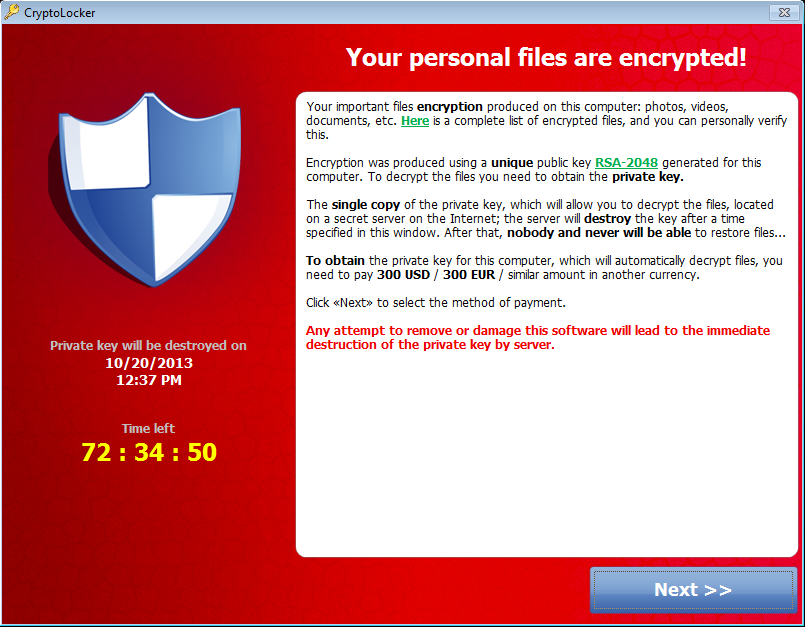
\includegraphics[width=.8\textwidth]{cryptolocker.png}
    \caption{Cryptolocker ransom message.}
    \label{fig:crypto_ransom}
\end{figure}

\paragraph{The Revenues} It is hard to provide a precise estimate of the
earnings that Cryptolocker brought to the attackers. \citeauthor{spagnuolo2013}
\footnote{Michele Spagnuolo is one of the most brilliant persons I have ever had
the chance to know and a friend of mine. Therefore it is a great pleasure of mine to cite
his work.} made a rough estimate of Cryptolocker earnings coming from the
Bitcoin payment system. In total they identified 771 ransoms, for 1,226 BTC (
approximately USD 1,100,000 on December 15, 2013)~\cite{spagnuolo2013}. Such a
measurement was addressed as ``conservative''. It is quite clear that the
Cryptolocker malware is to be considered of a very lucrative threat.


\paragraph{Conclusions} Cryptolocker is a very interesting example of malware
for a few reasons listed here below.
\begin{itemize}
    \item The primary infection vector is via a botnet: The fact that the attackers
        chose this vector lead us to think that in the future most of malware
        will be distributed in such a fashion.
    \item Cryptolocker forms itself a botnet: The network of infected machines
        communicate with the C\&C server in a centralized fashion, employing
        a DGA based rallying scheme.
    \item Being a \emph{ransomware} the malware of the year witnesses the
        attackers' paradigm shift, from no-profit malicious activities carried
        out for hacking interests to profitable ones, capable of massive earnings.
        ``Some men just want to watch the world burn'' is no longer an appropriate
        motto\footnote{The Dark Knight, 2008 Warner Bros.} to address the attackers.
    \item Attackers do not \emph{steal} sensitive personal data, but \emph{lock}
        computer files that, give the majority of targeted extensions, are likely
        to be the result of professionals' work, demonstrating a particular
        attention toward increasing the victims' willingness to pay.
\end{itemize}

All of the aforementioned reasons fully justify the focus of our work, as modern
miscreants' threats leverage the topology and communication scheme we have
tailored our software to search for.

% subsection cryptolocker (end)
% section botnets_a_modern_threat (end)


%-----------------------------------------------------------------------------%
% Summary
%-----------------------------------------------------------------------------%
\section{Summary} % (fold)
\label{sec:summary}
In this section we have introduced the phenomenon of botnets, one of today's most
spread and dangerous threats in computer security. We have briefly overviewed some of
the purposes carried out by these malicious infrastructures. We have explained why most
of these infrastructures feature a \emph{centralized} architecture and employ
a \emph{rallying} mechanism based on Domain Generation Algorithms to establish
the C\&C Channel, the communication medium used to \emph{i)} send orders to
the bots and \emph{ii)} retrieve harvested data or feedback from the bots.
Then we focused on the possible countermeasures to mitigate the threat: Both
sinkholing and takeover do need the C\&C server IP address to be played out.
Finally we have reported two real life cases of botnets in the wild, demonstrating
the threat danger and the actuality.
In the next chapter we focus on the problem we aim at contributing to resolve,
i.e., how to track down a botnet.
% section summary (end)

% chapter botnets (end)
    %!TEX root = ../thesis_polimi.tex

\chapter{Tracking down a Botnet} % (fold)
\label{chap:motivation}
\start{C}{hapter}~\ref{chap:botnets} gave an overview of
the phenomenon of botnets, which has become one of the most spread and remunerative
malicious activities on the Internet. Therefore it is of great interest for defenders to invest time and labor in finding new ways to mitigate them.
Given the primary architecture employed (centralized), the most effective way
to make a botnet harmless is to track down the C\&C Server and interrupt the
communication between the \emph{botmaster} and the \emph{bots}.

In this chapter we define the problem of interrupting a botnet
activities, present the \emph{state of the art} and
state the goals of our work  and the challenges we need to solve.

\paragraph{Chapter Organization} The remainder of this chapter is organized in the
following fashion:
\begin{itemize}
    \item in Section~\ref{sec:problem_statement} we precisely define the problem
        we want to address in this work;
    \item in Setion~\ref{sec:state_of_the_art} we present the most recent
        works in literature that cover this matter, highlighting the points
        of strength and the shortcomings, both starting point for \thesystem;
    \item in Section~\ref{sec:goals_and_challenges} we  elicit the goals we want
    to achieve with \thesystem and the challenges that have to be faced,
        highlighted in Setion~\ref{sec:state_of_the_art}.
\end{itemize}

\newpage

\section{Problem Statement} % (fold)
\label{sec:problem_statement}
\sectionstart{T}{racking} down and mitigating a botnet is the multi-faceted problem
that we wish to address. In the previous section we had an overview on the various
topologies, and highlighted how, though P2P botnets are growing, the centralized
architecture is still the most popular. Moreover we have explained how most of
them employ a \emph{rallying} mechanism based on DGAs.

In Section~\ref{sec:botnet_countermeasures} we have seen how the two most effective
countermeasures, \textbf{sinkholing} and \textbf{takeover} both aim at disrupting
the C\&C Communication Channel. To perform this task it is necessary to know the IP
address of the C\&C Server.\\
Therefore the problem of mitigating a centralized DGA-based botnet can be ``reduced''
to the task of finding the IP addresses of the C\&C servers that operate the
malicious infrastructure, though this operation is far from trivial.

In the next section we analyze the current state of the art.
Throughout this analysis we highlight the major shortcomings of the current
solutions and underline the importance of overcoming these limitations and
how \thesystem aims at achieving this goal.
% section problem_statement (end)


\section{State of the Art} % (fold)
\label{sec:state_of_the_art}
\sectionstart{B}{otnet} detection and, more generally, malicious activities
detection, by analyzing network data is a topic broadly covered in literature.
We focus on the detection of botnets that use DGAs to establish the
communication channel and on approaches that analyze high volumes of DNS data.

Works are presented in chronological order: Section~\ref{sub:detecting_malware_domains_upper} introduces \textsc{Kopis} by \citet{antonakakis2011}, which leverages three groups of features to distinguish
malicious domains from benign domains. Then, in Section~\ref{sub:exposure_finding_malicious_domains_using_passive_dns_analysis}, we report \textsc{Exposure}~\cite{bilge2011exposure}, a system that leverages large-scale passive DNS analysis
techniques to detect malicious domains.
\textsc{Disclosure}~\cite{bilge2012} is a system that aims at finding C\&C servers IP addresses by analyzing NetFlow data (see Section~\ref{sub:disclosure}).
In sections~\ref{sub:pleiades} and \ref{sub:early_detection_of_malicious_flux_networks_via_large_scale_passive_dns_traffic_analysis} we present two works, \cite{perdisci2012} \cite{antonakakis2012}, that
focus on the infected machines rather than on the C\&C servers, an approach that
leads to privacy and deployment difficulties. \citet{sharifnya2013} propose the
interesting approach of grouping together suspicious activities and then look
at their history to decide whether they are actually malicious or not (see Section~\ref{sub:a_novel_reputation_system_to_detect_dga_based_botnets}). \citet{haddadi2013malicious} focus on the detection of automatically generated domains
employed by DGA-based botnets, comparing different techniques that do not use
\emph{ad hoc} features, but leverage the domain name itself (see Section~\ref{sub:analyzing_string_format_based_classifiers_for_botnet_detection_gp_and_svm}). Finally in Section~\ref{sub:phoenix_detecting_dga_based_botnets} we present
\phoenix~\cite{schiavoni2013}, a system able to extract clusters of domains
related to DGA-based malicious activities from blacklists and a module
of \thesystem.


\subsection{Detecting Malware Domains at the Upper DNS Hierarchy} % (fold)
\label{sub:detecting_malware_domains_upper}
\citet{antonakakis2011} with \textsc{Kopis} were the first to monitor DNS activity at
the higher hierarchy level to detect domains related to malicious activities. It
leverages this uncharted point of view to explore new features later to be used to
train a supervised classifier.

\begin{description}
    \item[Requester Diversity] This group of features capture the geographical
        diversity of the hosts that query ad domain $d$. Malicious domains are usually
        queried by machines distributed differently from those querying legitimate
        domains~\cite{schiavoni2013}.
    \item[Requester Profile] This group of features aim at characterizing the
        different profiles of users that query DNS servers. Especially, it divides
        them into two broad categories: Those who reside in small networks, for instance a
        corporate network, and those who reside in large-scale networks. The insight
        is that while the latter should be more protected, as activity is usually
        better monitored in such infrastructures, the former are more
        likely to be exposed to and infected by malware.
    \item[Resolved-IPs Reputation] This group of features aims to describe whether,
        and to what extent, the IP address space pointed to by a given domain has been
        historically linked with known malicious services~\cite{antonakakis2011}.
\end{description}

\textsc{Kopis} lifetime is divided into \emph{training} and \emph{operation} mode.
During the first phase the system is fed with a set of known legitimate and
a set of known malware-related domains. For each domain the system computes a
feature vector that summarizes the domain behaviour in a time window of $m$ days.
Then, during \emph{operation} mode, \textsc{Kopis} builds a feature vector for each
unseen domain, capturing its behavior during a given epoch $E_j$. After the vector
is built it assigns a label (\emph{benign} or \emph{malicious}) to the unseen domain
and a confidence score.

\paragraph{Limitations} The main limitation of this work is the inability
to track down DGA-based botnets, as admitted by the authors themselves. This is caused by the short life span of the AGDs, which makes them untraceable by the
detection process implemented by \citet{antonakakis2011}. Moreover, the system is \emph{supervised}, as it requires initial
\emph{base knowledge} to be trained with.

% subsection detecting_malware_domains_upper (end)

\subsection{Detecting Malicious Activities by Passive DNS Analysis} % (fold)
\label{sub:exposure_finding_malicious_domains_using_passive_dns_analysis}
\citet{bilge2011exposure} in their work propose \textsc{Exposure}, a system that
classifies domain names as malicious or benign leveraging large-scale, passive
DNS analysis techniques. To achieve their goal, the authors first select 15 features
to discriminate between legitimate and malevolent traffic by feeding a J48 decision
tree with pre-labeled benign and malicious DNS traffic (i.e., DNS requests and
responses). The 15 features are grouped into four logical sets, reported here below.

\begin{description}
    \item[Time-Based Features] capture the peculiar time-related behaviors of
        malicious domains, for instance querying patterns, as high volume requests
        followed by a sudden decrease, typical of AGDs.
    \item[DNS Answer-Based Features] are four features related to the informations
        that can be retrieved querying a DNS server, as the number of distinct IP
        addresses resolved by a particular domain $d$.
    \item[TTL Value-Based Features] the \emph{Time To Live} expresses how much time,
        usually in seconds, a cached domain to IP mapping should be considered valid.
        In their research \citet{bilge2011exposure} found that usually malicious
        domains feature a low (less than 100s) TTL.
    \item[Domain Name-Based Features] are two features that aim at capturing the
        randomness of a domain name.
\end{description}

Then \citet{bilge2011exposure} train a supervised classifier to label domains as
malicious or benign, producing a blacklist of domain names--IP addresses, available
on their website\footnote{\url{http://exposure.iseclab.org/}}.

\paragraph{Limitations}
Even though able to produce a confirmed blacklist of malicious domains and IP addresses,
\textsc{Exposure} is a \emph{supervised} classification system which requires labeled data to be trained.
% subsection exposure_finding_malicious_domains_using_passive_dns_analysis (end)

\subsection{Detecting C\&C Servers by NetFlow data Analysis} % (fold)
\label{sub:disclosure}
\citet{bilge2012} propose \textsc{Disclosure}, a system that aims at finding C\&C
servers IP addresses by analyzing NetFlow data. The rationale behind this choice
resides in the lack of raw network data sources, motivated by administrative
and technical issues.
NetFlow is a network protocol by Cisco Systems for summarizing network
traffic as a collection of network flows~\cite{bilge2012}, where a network flow is
a unidirectional sequence of packets that share specific network properties.

\citet{bilge2012} individuate three classes of features that separate benign from
malicious network flows. The first one relates to the \emph{size} of the flow.
As miscreants' C\&C channels have been crafted with the goal of being resilient and
stealth, packets belonging to this flows tend to feature a small and constant size.
The second concerns the client access patterns. Infected machines will try to
contact the botmaster at fixed and regular intervals during the day, while benign
traffic exhibits a more ``random'' behavior. The last class of features captures the
\emph{temporal} patterns of access. Legitimate traffic tends to happen during
daylight, whilst malicious traffic does not feature this discrimination.

A \emph{Random Forest} classifier is fed with labeled data during the training
phase. Then it is tested against data from a university network and from a Tier 1
ISP.

\paragraph{Limitations} Even thought the use of NetFlow data is an interesting and
uncharted approach towards the unveil of C\&C servers, this approach shows some major
shortcomings. \textsc{Fire} \cite{stone2009fire}, \textsc{Exposure} \cite{bilge2011exposure} and Google Safe Browsing\footnote{\url{https://developers.google.com/safe-browsing/}} are reputations systems leveraged by the system to reduce the false positive rate,
otherwise unacceptable in volume of points, though low in percentage. Moreover the
selected features could be easily circumventable by an attacker. For instance he
could tell the bots to communicate during daylight. Or he could instruct them
to have a more ``random'' access behavior.
% subsection disclosure_detecting_botnet_command_and_control_servers_through_large_scale_netflow_analysis_leyla (end)

\subsection{Detecting FFSN by passive DNS data analysis} % (fold)
\label{sub:early_detection_of_malicious_flux_networks_via_large_scale_passive_dns_traffic_analysis}

\textsc{FluxBuster} was introduced by~\citet{perdisci2012} as a system able to detect
domains and IP addresses involved in the activity of FFSN, by analyzing DNS data
obtained by passively monitoring DSN traffic collected from ``above'' local RDNSs
servers~\cite{perdisci2012}.
The authors found four features that characterize DNS traffic belonging to this
threat: \emph{i)} a short TTL, \emph{ii)} high frequency in changing the resolving
IP addresses, \emph{iii)} high cardinality of the set of resolving
IPs~\cite{schiavoni2013} and \emph{iv)} the number of networks the IPs reside in.
\citet{perdisci2012} use these features to label new data as FFSN and non-FFSN
domains using a supervised classifier trained with labeled data.
The authors are able to distinguish domains belonging to malicious FFSN
from the benign ones, even if such a technique is used also for legitimate purposes
(CDN Networks), with a low false positive rate.

\paragraph{Limitations} \citet{perdisci2012} focus on the \emph{clients}, the
infected bots, rather than on the C\&C servers of the activities
(spam, phishing, etc.). Moreover their approach is \emph{supervised} and requires
previous knowledge.

% subsection early_detection_of_malicious_flux_networks_via_large_scale_passive_dns_

\subsection{Leveraging NXDOMAIN and clients' IP addresses} % (fold)
\label{sub:pleiades}
\citet{antonakakis2012} propose \textsc{Pleiades}, a system to \emph{i)} discover
and cluster together AGDs that belong to the same botnet, \emph{ii)} build
\emph{models} of such clusters and use this knowledge to \emph{iii)} classify unseen
domains.

During the first step, \emph{DGA Discovery}, \citet{antonakakis2012} analyze streams of
unsuccessful DNS resolutions, as seen from ``below'' a local DNS server~\cite{antonakakis2012}. The streams are collected during a given period of time, and then
clustered. The clustering is performed according to two criteria:
\begin{itemize}
    \item the statistical \emph{similarity} shared by domain name strings;
    \item the domains have been queries by overlapping sets of
        hosts~\cite{antonakakis2012}.
\end{itemize}
The final output of this module is a set of \texttt{NXDOMAIN} clusters: Each cluster is likely
to represent a DGA previously unknown or not yet modeled~\cite{antonakakis2012}.
After this stage is completed the system moves to the \emph{DGA Modeling} phase: This
module receives a labeled dataset of malicious and legitimate domains, and leverages
this knowledge to train the multi-class \emph{DGA Classifier}.

Then the \emph{DGA Classification} module aims at achieving two tasks. The first one
is to label a subset of a cluster of \texttt{NXDOMAIN}s with one of the labels seen in the
\emph{DGA Modeling} stage. The second is to trace back those domains that belong
to the clusters of \texttt{NXDOMAIN} but \emph{resolve} to an actual IP address, in order to
locate the C\&C Server.

\paragraph{Limitations} One limitation reside in the use of a HMM-based detector,
unable to detect certain types of DGAs, such as \texttt{Boonana}, as indicated by
the authors. Another shortcoming, also indicated by \citet{antonakakis2012},
is the possible scenario where the attackers produce on purpose random streams of
\texttt{NXDOMAIN} to sidetrack the detection system.
Moreover, once again, \textsc{Pleiades} requires \emph{i)} the clients' IP addresses
and subsequently \emph{ii)} DNS monitoring at the lower level, bringing in all the
privacy and deployment-related issues discussed above.
% subsection from_throw_away_traffic_to_bots_detecting_the_rise_of_dga_based_malware_manos (end)

\subsection{Leveraging activity history to detect botnets} % (fold)
\label{sub:a_novel_reputation_system_to_detect_dga_based_botnets}
\citet{sharifnya2013} developed a system to detect DGA-based botnet based on
features that include
the history of their activity. They aim at tracking down hosts infected by DGA-based
botnets by leveraging DNS queries and trying to group together hosts that exhibit
similar malicious behaviors.

The first step is to \emph{whitelist} the DNS queries, filtering
out those domains that appear in the Alexa TOP 100 list (list of the most 100 popular
domains on the Internet by volume of queries).

Then \citet{sharifnya2013} group together those domains that \emph{i)} resolve to
the same IP address or \emph{ii)} have the same Second Level Domain (SLD) and TLD. After a time window
they label as suspicious those groups where domains are automatically generated. To
establish whether a domain is automatically generated, they first compute
the distributions of 1-gram and 2-gram for Alexa TOP 1,000,000 sites and the
malicious domain names from Murofet~\cite{sharifnya2013}. Then they leverage the
\emph{Kullback-Leibler divergence} and the \emph{Spearman's rank correlation
coefficient} to tell to which category a domain name belongs to.

Simultaneously, another building block of their system, called \emph{Suspicious
Failure Detector}, triggers and flags the host as suspicious when a high volume
NXDOMAINS DNS queries is originated.
Finally, the results from the previous blocks are combined by the \emph{Negative
Reputation Calculator}, responsible of the final verdict, i.e., tell whether a host
shall be considered bot-infected or not.

\paragraph{Limitations} The idea of grouping together suspicious activities and leveraging their history will be
borrowed and, in our opinion, enhanced by \thesystem.
Even in light of the positive results shown
by the authors, this work suffers from two major shortcomings. First the system needs
a feed of malicious domains automatically generated to compute the
malicious distributions of \emph{n}-grams, resulting vulnerable to DGAs that exhibit a new and different distribution of \emph{n}-grams. Second this is an approach
\emph{host-based}, which requires the DNS query with the client IP address. This
choice involves all the difficulties related to privacy issues and, consequently,
leads to non-repeatable experiments~\cite{rossow2011} and deployment difficulties already
discussed in~\cite{schiavoni2013}.
% subsection a_novel_reputation_system_to_detect_dga_based_botnets (end)

\subsection{Using SVM and SSK to classify AGDs} % (fold)
\label{sub:analyzing_string_format_based_classifiers_for_botnet_detection_gp_and_svm}
\citet*{haddadi2013} focus on detection of automatically generated domains employed
by DGA-based botnets. In their work they compare with other techniques a genetic
programming approach, result of their previous work~\cite{haddadi2013malicious}, to detect
malicious domain names, based only on the string format, i.e., the raw domain name
string. This is quite important as to the best of our knowledge, all detection
systems in this field analyze DNS network traffic behaviour via classifiers with
pre-defined feature sets~\cite{haddadi2013}.
We briefly compare the techniques and motivate why we chose the Support Vector Machine
approach in \thesystem.

The first technique to be introduced relies upon Support Vector Machines,
state of the art classifiers in many supervised learning tasks. A Support Vector
Machine finds a hyperplane that optimally separates the points of the dataset in two
classes. This technique can be employed to perform $k$-classes classification by
building $k$ binary classifiers. The machine needs a Kernel Function to be able
to separate data which is not-linearly separable. \citet{lodhi2002} proposed the
Subsequence String Kernel, a kernel based on common substrings to determine strings'
similarity. Once the SVM is equipped with the kernel it must be trained with an initial
dataset and then it is ready for classification.

In the authors' Stateful-SBB approach there are
three populations that coevolve: A point population, a team population and a learner
population. The point population consists of a subset from the training data samples.
The learner population represents a set of symbionts, which relate a GP-bidding
behaviour with an action~\cite{haddadi2013}. Finally, in the team population we find
a set of learners. The evolution follows a Pareto competitive coevolution.

The authors trained the classifier to distinguish between three
classes of domains, two malicious and one benign. Conficker and Kraken were chosen as
representative of the domains devoted to botnets' C\&C communication, while 500 benign
domains were manually extracted from the Alexa list. The results favor the SVM
approach, which features the highest score ($0.996$) and a training time ($431.53$) one order of magnitude less than the SBB approach ($2227.64$).

\paragraph{Limitations} \citet{haddadi2013} strongly improve previous features based
classifiers, leveraging only the \emph{raw} string of the domain name. Nevertheless
their work suffers from being a \emph{supervised} approach. In fact the system must
be trained using AGDs blacklist, and it is not capable of detecting new threats.
Nevertheless this work lead us to consider the SVM approach when we had to design and implement our
classifier, for two main reasons: \emph{i)} in~\cite{haddadi2013} it is the best tool to perform such a task, with performances close to
perfection, \emph{ii)} employing the String Subsequence Kernel as system-wide metric to be used by the DBSCAN clustering routine (see Par.~\nameref{par:dbscan_clustering} in Section~\ref{ssub:the_time_detective})
to perform similarity calculations between domains and cluster of domains. Such matters
shall be more deeply discussed in Chapter~\ref{chap:approach}.
% subsection

\subsection{Phoenix, Detecting DGA-based botnets} % (fold)
\label{sub:phoenix_detecting_dga_based_botnets}
\citet{schiavoni2013} proposed \phoenix, a system able to extract clusters of domains related to DGA-based
malicious activities from blacklists. To this end, \phoenix first separates
domains automatically generated from those created by humans, by leveraging a
vector of linguistic features. These linguistic features are \emph{i)} the
\emph{meaningful word ratio}, i.e., the ratio of domain's characters composing
meaningful words to the cardinality of the domain itself and \emph{ii--iv)}
the \emph{popularity score} of the \emph{n}-grams, with \emph{n} ranging from
one to three. We shall better explain these concepts via an example. Consider the
domain names \texttt{facebook.com} and \texttt{pub03str.info}. Let us compute the
\emph{meaningful word ratio} for both of them (see Figure~\ref{fig:words_ratio}).

\begin{figure}[!htp]
    \begin{minipage}{0.5\linewidth}
        \centering
        $$ d = \mathtt{facebook.com}$$\vspace{-0.2cm}
        $$R(d) = \frac{|\mathtt{face}| +|\mathtt{book}|}{|\mathtt{facebook}|} = 1$$
        \vspace{0.3cm} \\ likely \bfseries{HGD}
        \end{minipage}\begin{minipage}{0.5\linewidth}
        \centering
        $$ d = \mathtt{pub03str.info}$$\vspace{-0.2cm}
        $$R(d) = \frac{|\mathtt{pub}|}{|\mathtt{pub03str}|} = 0.375.$$
        \vspace{0.3cm} \\ likely \bfseries{AGD}
    \end{minipage}
    \caption{Meaningful Word Ratio example, \citet{schiavoni2013}.}
    \label{fig:words_ratio}
\end{figure}

The domain \texttt{facebook.com} scores 1, as all of the characters in the domain
name contribute to form the words \texttt{face} and \texttt{book}, which can
be found in the English language dictionary. The high score indicates that we have a domain which is likely a Human Generated Domain (HGD). On the other hand, in the domain name
\texttt{pub03str.info} the only meaningful substring is \texttt{pub} and the
\emph{meaningful word ratio} is equal to 0.375, likely an AGD.

Consider now the domain names \texttt{facebook.com} and \texttt{aawrqv.com} and let
us compute the popularity score of the 2-gram (see Figure~\ref{fig:two_gram_example}).

\begin{figure}[!htp]
\begin{minipage}{0.5\textwidth}
    \centering
    $$ d = \mathtt{facebook.com}$$\vspace{-0.2cm}
    \begin{scriptsize}
        \begin{tabular}{c c c c c c c}
          \texttt{fa} & \texttt{ac} & \texttt{ce} & \texttt{eb} & \texttt{bo}  & \texttt{oo}  & \texttt{ok}\\
          109 & 343 & 438 & 29 & 118 & 114 & 45
        \end{tabular}\end{scriptsize}\\
        \vspace{0.5cm}
        mean: $S_2 = 170.8$
        \vspace{0.3cm} \\ likely \textbf{HGD}
\end{minipage}%
\begin{minipage}{0.5\textwidth}
        \centering
        $$ d = \mathtt{aawrqv.com}$$\vspace{-0.2cm}
        \begin{scriptsize}
        \begin{tabular}{ c c c c c }
          \texttt{aa} & \texttt{aw} & \texttt{wr} & \texttt{rq} & \texttt{qv}\\
          4 & 45 & 17 & 0 & 0
        \end{tabular}\end{scriptsize}\\
        \vspace{0.5cm}
        mean: $S_2 = 13.2$
        \vspace{0.3cm} \\ likely \textbf{AGD}
\end{minipage}
\caption{2-gram score example, \citet{schiavoni2013}.}
\label{fig:two_gram_example}
\end{figure}

The popularity is computed by counting the number of occurrences of the domain's
substrings in the English language dictionary. This score captures the
\emph{pronounceability} of a domain name: The more the times a \emph{n}-gram
is found in the dictionary, the higher the score, the easier should be to
pronounce the domain name. For instance, the \texttt{oo} 2-gram is very common
in the English dictionary as it is a common sound in the English language.
In our example \texttt{facebook.com} features a high score and it is therefore
likely to be a HGD, while \texttt{aawrqv.com} features a low score and it is
therefore likely to be an AGD.

All of the four aforementioned features are combined into a feature vector
$\vec{f}$, which is computed for every domain belonging to the Alexa Top
100,000 domains list, which lists the 100,000 most popular domains on the web,
all very likely to be domain names generated by humans. Then \citet{schiavoni2013}
computed the centroid over this group of domains. The idea is that if a
domain is farther than a certain threshold $\lambda$, then it is likely to be
automatically generated.

The algorithm described above is used to separate the HGDs from the AGDs in a
blacklist of malicious domains. Then the subset of AGDs is used to generate
clusters of domains, depending on the IP they resolve to. Hopefully such IP
addresses belong to the C\&C servers responsible of controlling the malicious
activity the domains refer to.
Once the clusters have been generated, \phoenix uses a list of features to
compute clusters' models to be used for classification of unseen domains.
The goal is to label unseen domains with one of the threats identified in
the clustering phase.

\paragraph{Limitations}
There are two major limitations in \phoenix, the first \emph{conceptual} while the
second concerns the system's validation. The \emph{conceptual} limitation resides
in the features used to classify unseen domains. One of these features is the
IP address of the C\&C servers, which means that if an unseen domain does not
share the IP address with one of the clusters it is not considered malicious.
Obviously this is not true, as actually attackers do change the location
of the C\&C server once they are identified. Moreover, other two features
used by \citet{schiavoni2013} are the length of the domain and the TLD. This means
that if an attacker decides to use a DGA that makes domains longer or shorter
than usual, or domains that exhibit a different TLD, \phoenix does not
label them as belonging to the threat they actually belong to.
The other limitation has to do with how the system was validated.
\citet{schiavoni2013} did not test \phoenix in the wild, whereas
the purpose of a detection system is to detect threats analyzing real world
data.

% subsection phoenix_detecting_dga_based_botnets (end)
% section state_of_the_art (end)


\section{Goals and Challenges} % (fold)
\label{sec:goals_and_challenges}
\sectionstart{O}{ur} primary goal is to isolate in an automatic and unsupervised fashion DGA-based botnets, clustering malicious activities that use the same DGA, by analyzing DNS passive data, in order to unveil botnets' C\&C servers IP addresses,
as to make it possible to apply the required countermeasures.

Most systems described above, ~\cite{haddadi2013}~\cite{sharifnya2013}~\cite{antonakakis2011}~\cite{antonakakis2012}~\cite{perdisci2012}~\cite{bilge2012},
suffer from the \emph{supervised} approach. We think
that in this particular scenario this is a major issue: We would like our system to
be able to detect \emph{new} threats with little or no previous knowledge.
Other systems, \cite{antonakakis2012}~\cite{sharifnya2013}, leverage the \emph{clients'} (i.e., the \emph{bots'})
IP addresses to cluster together DNS traffic that relates to the same malicious
activities. This approach falls into the privacy related issues that arise when
dealing with this kind of data. Moreover the monitors to get these samples must be
located at the lower levels of the DNS hierarchy, which causes difficulties in
the deployment of the monitors themselves.
One system, \textsc{Pleiades}~\cite{antonakakis2012} does not perform well with some
types of DGAs (e.g., \texttt{Boonana}),
whereas we want to build a detection software that does not leverage \emph{some}
features of peculiar DGAs.

\phoenix~\cite{schiavoni2013} is the system that meets most of our criteria, as
it uses an \emph{unsupervised} approach and analyzes passive DNS data, free of
any privacy issues.
Still, it shows some major shortcomings, as the impossibility of detecting
unknown botnets, the fact that the classifier is not resilient to
small modifications in the DGAs and the lack of a validation in the wild, which
makes us agnostic with respect to \phoenix's effectiveness once deployed in the real
world.

Building a system that evolves in an automatic and unsupervised fashion constitutes a hard challenge to face.
We have to find a way to filter out benign domains while keeping the malicious
domains that does not require knowledge to be fed, i.e., we have to think about
general features that characterize malicious AGDs. Moreover this filtering
process must be fast enough to allow an online detection process while dealing
with high volumes of data.
We also need to understand how to cluster together domains that look ``similar'',
therefore we have to develop a concept of similarity between domain names
(i.e., strings) that is able to capture the patterns shared by AGDs produced
by the same DGA. Once the malicious activities are clustered, we need to
understand how we can use this knowledge to build a classifier that is
resilient to small changes in the DGA and does not use \emph{ad hoc} features.
The previous challenges brought to the birth of \thesystem, which shall be
presented in Chapter~\ref{chap:approach}.
% section goals_and_challenges (end)
% chapter motivation (end)
    %!TEX root = ../thesis_polimi.tex

\chapter{Introducing Cerberus} % (fold)
\label{chap:approach}

\start{C}{erberus} or Kerberos (Κέρβερος) is a three-headed guardian dog from the Greek mythology, in charge of
patrolling the gates of Hades, land of the dead. Preventing dead souls to evade the
underworld was his duty. In the same fashion we wanted to build a tool to \emph{detect}
malicious domains employed by botnets and track down the IP addresses these domains resolve
to, as to guarantee that they shall not tarnish the namespace ever again.

As the hellhound featured three heads, our \thesystem operates in three
phases: The \important{Bootstrap Phase}, where the initial optional ground truth is
generated, the \important{Filtering Phase}, where the DNS data is filtered, and the
\important{Detection Phase}, where domains are classified and new threats are
discovered.

\paragraph{Chapter Organization} The remainder of this chapter is organized in the
following fashion:
\begin{itemize}
    \item in Section~\ref{sec:approach_overview} we will describe \thesystem at
        a high level of abstraction, providing an overview of the overall process;
    \item in Section~\ref{sec:approach_details} we will tackle all the
        elements that form \thesystem.
\end{itemize}

\newpage

\section{Cerberus Overview} % (fold)
\label{sec:approach_overview}
\sectionstart{C}{erberus} is composed of three main modules or phases: \important{Bootstrap},
\important{Filtering} and \important{Detection} (see Figure~\ref{fig:cerberus_overview_approach}). The \important{Bootstrap Phase} is fed with a blacklist of malicious domains and
provides the initial ground truth to the system in an automatic and unsupervised fashion. We use the term \emph{ground truth} to refer to the knowledge that the
system trusts even though its correctness was not validated by any external authority.
The ground truth consists of a set of clusters of domain names and the IP addresses they
resolve to, clusters that represent DGA-based malicious activities employing the same DGA.
This knowledge is used by the \important{Detection Phase}.

\begin{figure}[!htp]
    \centering
    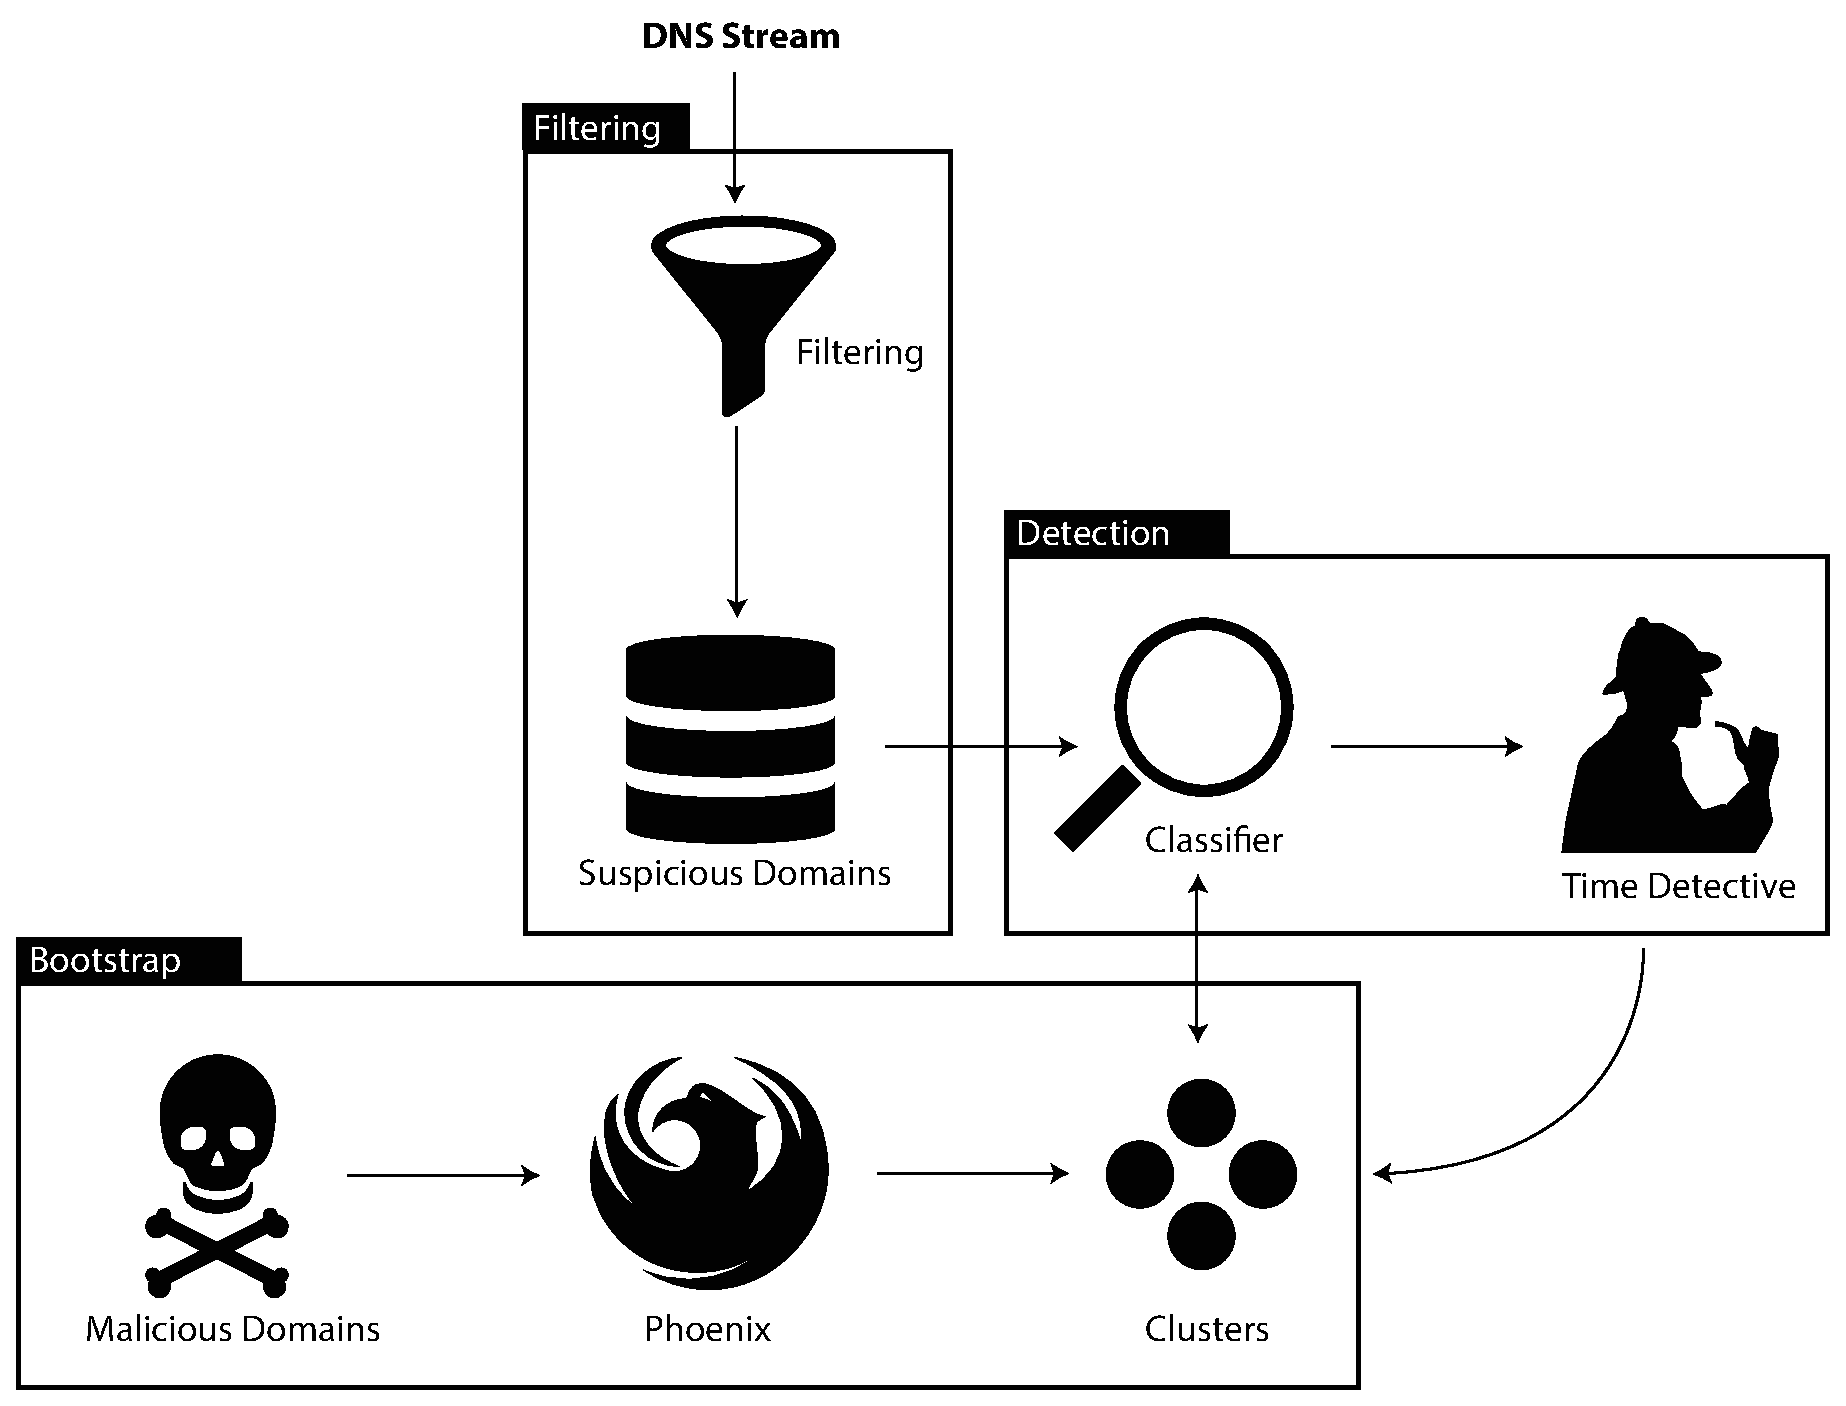
\includegraphics[width=\linewidth]{cerberus.eps}
    \caption{Cerberus overview.}
    \label{fig:cerberus_overview_approach}
\end{figure}

The \important{Detection Phase} consumes the output of the \important{Filtering Phase}, where a stream of
DNS replies is filtered to obtain a list of likely malicious domains. To this end
we employ a list of filters mostly based on heuristics and whitelists to reduce as
much as possible the number of legitimate domains, while keeping the suspicious
ones.
After the \important{Filtering Phase} is completed, the Classifier uses the
ground truth previously generated to \emph{detect} known threats, i.e., the Classifier returns a list of malicious domains labeled with one of the clusters from the ground truth. To this end,
for each unseen domain it selects those clusters that share the domain IP address
and then decides to which one  it should be assigned using a Support Vector Machine that leverages the Subsequence String Kernel to compute similarity between strings.

Those domains that do not share their IP address with the ground truth are fed to
the \textbf{Time Detective}: The rationale is that at this very moment we cannot establish whether these ``suspicious'' domains are actually malicious, but by analyzing the activity related to their IP addresses we may be able to correctly identify the threats. The \textbf{Time Detective} stores the ``suspicious'' IP addresses
and keeps track of the domains that resolve to them throughout time. After $\Delta$ time has passed it groups them by their Autonomous System,
and clusters together the domains that are deemed similar (see Section~\ref{par:dbscan_clustering}).
After the new clusters are generated they are added to the ground truth and this
further knowledge is then used to increase the range of detected threats.

\begin{figure}[!htp]
    \centering
    \begin{tikzpicture}
        \node (DETECTION) {Detection};
        \node[above left=1cm of DETECTION] (BOOTSTRAP) {Bootstrap};
        \node[below right=of DETECTION,minimum height=3em] (CLUSTERING) {Clustering};
        \node[below left=of DETECTION, align=center, minimum height=3em] %
            (KNOWLEDGE) {Increase\\Knowledge};
        \node[below=3.3cm of DETECTION] (DISCOVER) {Discover};

        \node [right=0cm of CLUSTERING]  {
\includegraphics[width=.6cm]{detective.eps}};
        \node [below=0cm of DETECTION]  {
\includegraphics[width=.6cm]{classifier.eps}};
        \node [left=0cm of BOOTSTRAP]  {
\includegraphics[width=.6cm]{phoenix.eps}};
        \node [left=0cm of KNOWLEDGE]  {
\includegraphics[width=.6cm]{knowledge.eps}};

        \path[arrow]
            (BOOTSTRAP.east)  edge[bend left] (DETECTION.north)
            (DETECTION)  edge[bend left]  (CLUSTERING)
            (CLUSTERING) edge[bend left] (DISCOVER)
            (DISCOVER)   edge[bend left] (KNOWLEDGE)
            (KNOWLEDGE)  edge[bend left] (DETECTION)
        ;
    \end{tikzpicture}
    \caption{Cerberus lifecycle.}
    \label{fig:cerberus_lifecycle}
\end{figure}

This process is summarized in Figure~\ref{fig:cerberus_lifecycle}: \thesystem can automatically evolve by increasing its
knowledge in an unsupervised fashion: The Clustering routine allows to discover
new threats that are added to the ground truth. Then the system can return in
the \important{Detection Phase}, leveraging the new knowledge.
In the next section we discuss in further detail what briefly described above.
The symbols used in Figure~\ref{fig:cerberus_overview_approach} will provide a visual aid
to better understand which part of the schema we will be describing.
% section approach_overview (end)

\newpage

\section{Cerberus Details} % (fold)
\label{sec:approach_details}
\sectionstart{I}{n} the previous section we have given a brief overview of how
\thesystem works. In the following of this section, we shall go in deeper detail,
throughly explaining every aspect of the \important{Bootstrap}, \important{Filtering}
and \important{Detection} phases.

\subsection{The Bootstrap Phase} % (fold)
\label{sub:the_bootstrap_approach}
\begin{wrapfigure}{l}{2.2cm}
\centering
    
\includegraphics[width=2cm]{phoenix.eps}
\end{wrapfigure}
The \important{Bootstrap Phase} aims at providing \thesystem with the initial ground
truth. This knowledge is not mandatory to have, as the system needs no \emph{a
priori} knowledge to start detecting new threats. Nevertheless it is useful to have
the possibility to plug it into \thesystem, which can use it to label the unseen domains during the \important{Detection Phase}. To this end we employ
\phoenix. \phoenix takes as initial input a list of malicious domains. It then
applies a DGA filter (the same used in Paragraph~\ref{par:phoenix_dga_filter})
to filter out those domains that appear likely benign, under the assumption that domains generated manually, by a human, are benign, in contrast to AGDs, which are generated automatically by a DGA. Therefore
the remaining domains are both \emph{non-benign} (i.e., suspicious) and \emph{automatically generated}.

\thesystem clusters these domains depending on the IP address(es) they resolve to. Hence
at the end of the clustering process, \thesystem has a list of clusters of domains
and the IP addresses they resolve to, domains produced by the same DGA and IP
addresses that should belong to the C\&C servers, and it will later leverage this
list to label unseen domains in the \important{Detection Phase}.

\dataexample{%
    \parbox{.9\textwidth}{
    The following are two of the eleven clusters generated by the
    \important{Bootstrap Phase}:}
    \vspace{.1cm}
    \begin{center}
    \begin{minipage}{.5\textwidth}
            \centering
            \begin{tabular}{rp{2.8cm}}
            \multicolumn{2}{l}{\textsc{Cluster f105c}} \\
            \midrule
            Threat: & Palevo \\
            IPs: & \texttt{176.74.176.175} \newline \texttt{208.87.35.107} \newline \newline \\
            Domains: & \texttt{cvq.com} \newline \texttt{epu.org} \newline \texttt{bwn.org} \\
            \end{tabular}
        \end{minipage}%
        \begin{minipage}{.5\textwidth}
            \centering
            \begin{tabular}{rp{2.8cm}}
                \multicolumn{2}{l}{\textsc{Cluster 0f468}} \\
                \midrule
                Threat: & Sality \\
                IPs: & \texttt{217.119.57.22} \newline \texttt{91.215.158.57} \newline \texttt{178.162.164.24} \newline \texttt{94.103.151.195} \\
                Domains: & \texttt{jhhfghf7.tk} \newline \texttt{faukiijjj25.tk} \newline \texttt{pvgvy.tk} \\
            \end{tabular}
        \end{minipage}
    \end{center}
}

% subsection the_bootstrap (end)

\subsection{The Filtering Phase} % (fold)
\label{sub:the_filtering_phase}
\begin{wrapfigure}{l}{2.2cm}
\centering
    
\includegraphics[width=2cm]{filter.eps}
\end{wrapfigure}
After the \important{Bootstrap Phase}, \thesystem aims at classifying unseen
domains from a stream of DNS passive data.
The DNS stream we receive comes from the real world, hence it features both benign and malicious
domains. Therefore we want to reduce as much as we can the amount of legitimate domains
while keeping as many malicious domains as possible. To achieve this goal the DNS feed goes
through a list of filters listed here below.

\paragraph{Alexa Whitelist} % (fold)
\label{par:alexa_whitelist}
This filter removes all the domains that rank amongst the first 1,000,000 in the Alexa Top
Domains list. The rationale is that the most popular domains in the Web are less likely to be malicious.
Even though this is not completely true (as of 2012, BarracudaLabs found 58 drive-by-download
malicious websites in the first 25,000 Alexa domains\footnote{\url{https://media.blackhat.com/ad-12/Royal/bh-ad-12-quanitfying-royal-slide.pdf}}), there are no known cases of malicious AGDs found among the Alexa Top 1M. Moreover we are looking for domains
used to set up the C\&C channel: They are usually valid for one day and then thrown away and
it is very unlikely that they make it to the list.
% paragraph alexa_whitelist (end)

\paragraph{Content Distribution Networks} % (fold)
\label{par:content_distribution_networks}
DGAs are used to legitimate ends by Content Delivery Networks (CDNs). These
infrastructures consist of a large distributed system of servers, deployed with the
intention of providing users with content at high availability and high performance.
YouTube and Amazon CloudFront are examples of this type of networks. In our system we
filled in a list of the most popular CDNs: If a domain belongs to one of them it is
filtered out. For instance, the domain \texttt{r4---sn-a5m7lnes.c.youtube.com}
belongs to the YouTube CDN: It was clearly generated by some DGA, but it is not
malicious and therefore it must be filtered out.
% paragraph content_distribution_networks (end)

\paragraph{Top Level Domain Whitelist} % (fold)
\label{par:top_level_domain_whitelist}

Some TLDs require clearance before the domain can be registered (see Table~\ref{tab:tlds_clearance}). When the attackers register their domains they do not want to go through authorizations
by third party authorities, for two obvious reasons: \emph{i)} they do not want anyone to
investigate the domain they are going to register and \emph{ii)} they cannot wait for the time required by
clearance process. Therefore all of those domains that feature a TLD listed in Table~\ref{tab:tlds_clearance} are filtered out.

\begin{table}[!htp]
    \centering
    \begin{tabular}{rp{4cm}rp{4cm}}
        \toprule
        \textsc{TLD} & \textsc{Entity} & \textsc{TLD} & \textsc{Entity} \\
        \midrule
        \texttt{.ac.uk} & British academic\newline domains & \texttt{.edu} & educational \\
        \texttt{.aero} & air-transport industry   & \texttt{.gov} & governmental \\
        \texttt{.arpa} & Address and Routing \newline Parameter Area & \texttt{.int} & international \newline organizations \\
        \texttt{.coop} & cooperatives & \texttt{.mil} & US Military \\
        \texttt{.museum} & museums & \texttt{.pro} & professions \\
        \texttt{.post} & postal services & \texttt{.travel} & travel and tourism \newline industry \\
        \bottomrule
    \end{tabular}
    \caption{TLDs requiring clearance before registration.}
    \label{tab:tlds_clearance}
\end{table}
% paragraph top_level_domain_whitelist (end)

\paragraph{Time To Live} % (fold)
\label{par:time_to_live}
The TTL parameter sets for how long a cached DNS record is to be considered valid in a local
DNS Server. Previous works in literature (\cite{bilge2011exposure}, \cite{holz2008})
stated that this value was set to very low values (100s) in the case of malicious
domains. The rationale, from the botnet operators, is that these infrastructures need to update fast their C\&C locations and therefore need the DNS server to update the records at the same pace. However, more recent investigations seem to state the
opposite. \citet{xu2013} from Palo Alto Networks reported that approximately 80\%
of fast-flux domains exhibit a change rate greater than 30 minutes/IP, while in
2008 \citet{holz2008} reported that fast-flux domains
exhibited a changing rate less than 10 minutes/IP. This change, and the subsequent
change in TTL values, is due economic reasons and to avoid detection based on
changing rate. Therefore we decided to filter out all the domains featuring a low
TTL value, less than 300 seconds. We chose this value after analyzing two weeks
of DNS data from the ISC/SIE dataset in our possession: We manually searched for
the domains classified as malicious by an early version of \thesystem, and noticed
that all the benign domains featured a TTL equal or lower than 300 seconds.
% paragraph time_to_live (end)

\paragraph{\phoenix DGA Filter} % (fold)
\label{par:phoenix_dga_filter}
The domains employed in DGA-based malicious activities feature that randomness captured
by \citet{schiavoni2013} in \phoenix. Therefore we filter out those domains that do
not exhibit the required level of randomness to be labeled as AGDs.
% paragraph phoenix_dga_filter (end)

\paragraph{Whois Queries} % (fold)
\label{par:whois_queries}
Finally we look at the registration date. We leverage the insight that attackers
do not (and sometimes \emph{cannot}, as when using unpredictable seed in the DGA, e.g., Twitter trend topic) register
their domains much time in advance, as otherwise they would
not be able to leverage the resilient migration strategy allowed by the use of DGAs:
If the C\&C is unveiled they should update the DNS records for all the
pre-registered domains.

Therefore we query a \texttt{Whois} server to ask for the registration date of every domain:
If the domain is ``old'' it is discarded, whereas if either it was recently registered or
the \texttt{Whois} server replied with an error code (e.g., no information is available for that domain), we conservatively keep the domain. For all the
retained domains we
store the registration date for later use in the detection phase.
% paragraph whois_queries (end)

\paragraph{Summary} % (fold)
\label{par:summary}
We want to recap here the features of the domains that remain at the end of the
filtering process and that constitute the input for the \important{Detection Module}.
For each step we report also the number of domains that persist after the filtering
process in a pilot experiment conducted on 30' of sampled traffic (see Section~\ref{sec:dataset}).


\begin{description}[labelwidth=\widthof{20,000}, leftmargin=!, align=parright]
    \item[20,000] domains remain with a TTL greater than 300 seconds;
    \item[19,000] domains not in the Alexa Top 1M whitelist;
    \item[15,000] domains not in the most popular CDNs;
    \item[800] domains likely to be AGDs;
    \item[700] domains featuring a TLD that does not require previous authorization;
    \item[300] domains that have been recently registered.
\end{description}

% paragraph summary (end)

% subsection the_filtering_phase (end)

\subsection{The Detection Phase} % (fold)
\label{sub:dga_detection}
In the \important{Detection Phase}, we aim at recognizing domains belonging to known botnets
and to discover new ones. These two tasks are achieved by two different modules: The
\important{SSK Classifier} and the \important{Time Detective} respectively.

\subsubsection{The Subsequence String Kernel Classifier} % (fold)
\label{ssub:ssk_classifier}
\begin{wrapfigure}{l}{2.2cm}
\centering
    
\includegraphics[width=2cm]{classifier.eps}
\end{wrapfigure}
This component is fed with the data coming from the \important{Filtering Phase}.
It classifies each unseen domain domain $d$ using the knowledge provided
by \phoenix, i.e., the clusters of DGAs, eventually including those generated by \thesystem. The classifying process consists of assigning
$d$ to one of those clusters.
\citet{schiavoni2013} had developed their own classifier, but it suffered from the major
shortcoming of using \emph{ad hoc} parameters, such as the domain length and the TLD.
This means that if $d$ features a TLD other than those in the clusters, or if it
features a length that does not reside in the previously seen boundaries, it is discarded.

We wanted to have a classifier resilient to such changes, one that would label $d$ leveraging
only the \emph{string} itself as a feature to compute similarity amongst $d$ and the clusters.
\citet{haddadi2013malicious} compared different approaches in classifying AGDs: As the Support
Vector Machine technique outplayed all the others with respect to the F-Score,
we decided to use this approach.

\paragraph{Support Vector Machines} % (fold)
\label{par:support_vector_machines}
The Support Vector Machine is a binary learning machine that can be used for classification
and rule regression~\cite{alpaydin2004introduction}. The main idea of this classification
algorithm is to build a hyperplane that optimally separates the samples of data into two
categories with maximal margin~\cite{haddadi2013malicious}. It is possible to build a
\emph{k}-classes classifier, with $k$ greater than two, by building $k$ binary classifiers.

Support Vector Machines must undergo a \emph{training phase}, where they are fed with points
in the form of $\{\vec{x_i}, y_i\}$, where $\vec{x_i}$ is a feature vector and $y_i$ is the
binary class label (e.g., $1$ or $-1$). Note that in our context, the labels need not to be provided manually because we use clusters as labels, which are generated automatically. There is a parameter to be set during the classification process:
$C$, which controls the punishment function for misclassified points. In our implementation
we left this parameter to 1, its default value.

When dealing with linear data we have to
find two hyperplanes:
\[ \vec{w} \cdot \vec{x} -b = 1\]
\begin{center}
and
\end{center}
\[ \vec{w} \cdot \vec{x} -b = -1\]
that bound a region, called \emph{the margin}, where no data point is present. Training the
SVM in this case means to maximize the distance between the hyperplanes.
SVMs can be also employed to classify data that are non-linearly separable, but they need to
be equipped with a \emph{kernel function}, a non-linear mapping of an input data into a high
dimensional feature space~\cite{haddadi2013malicious}. When the mapping is completed, the
hyperplane that maximizes the separation margin can be constructed. Then, as a final step,
a linear mapping from the feature space to the output space is required~\cite{haddadi2013malicious}. In the next paragraph we shall better explain what a kernel function
is and introduce the Subsequence String Kernel.

% paragraph support_vector_machines (end)

\paragraph{Subsequence String Kernel} % (fold)
\label{par:subsequence_string_kernel}
A function that calculates the inner product between mapped examples in a feature space
is a kernel function~\cite{lodhi2002}. Therefore for any mapping:
\[ \phi \; : \; D \rightarrow F \]
we define a kernel function as
\[ K(d_i, d_j) = \langle \phi(d_i), \phi(d_j) \rangle \]
where $\langle \cdot , \cdot \rangle$ is the dot product and $d_i$, $d_j$ are feature vectors.
In 2002 \citet{lodhi2002} proposed a kernel function to measure the similarity of strings.
The idea is to compare them by means of the substrings they contain: The more substrings
in common, the more similar they are~\cite{lodhi2002}. We can better explain the process
by looking at the example in Table~\ref{tab:SSK}.

\begin{table}[!htp]
    \begin{minipage}{.5\textwidth}
    \begin{tabular}{lacccc}
                        & c-a         & c-t         & a-t         & c-r          & a-r         \\
        \midrule
        $\phi($cat$)$   & $\lambda^2$ & $\lambda^3$ & $\lambda^2$ &  0           & 0           \\
        $\phi($car$)$   & $\lambda^2$ & 0           & 0           &  $\lambda^2$ & $\lambda^2$ \\
    \end{tabular}
    \end{minipage}%
    \begin{minipage}{.5\textwidth}
        \begin{align*}
        \text{ker}(car,cat) &= \lambda^4 \\
        \text{ker}(car,car) &= \text{ker}(cat,cat) = 2\lambda^4 + \lambda^6 \\
        \text{ker}(car,cat) &= \frac{\lambda^4}{(2\lambda^4 + \lambda^6)} = \frac{1}{(2 + \lambda^2)}
    \end{align*}
    \end{minipage}
    \caption{SSK example from \citet{lodhi2002}.}
    \label{tab:SSK}
\end{table}

We consider the two strings \texttt{car} and \texttt{cat}. The first step is to compute the feature space of the strings to be compared.
In this case it is a 5-dimensions space composed by the features \texttt{c-a}, \texttt{c-t},
\texttt{a-t}, \texttt{c-r} and \texttt{a-r}, which are all the possible non-contiguous
 two characters long substrings of \texttt{car} and \texttt{cat}.

We then set a \emph{decay factor} $\lambda$ that measures a decay in the quality of the
similarity between strings, i.e., if we have $\lambda^n$, it means that we need $n$
characters of the string to match the substring. In our example we have for instance
\texttt{c-t}, which is present in \texttt{cat}, but it requires three characters to be
matched: \important{c}, a and \important{t}. That is why we then find $\lambda^3$ in the
cell ($\phi(\text{cat})$, \texttt{c-t}).

We then define the inner product between two strings $s$ and $t$ as the sum over all common
subsequences weighted according to their frequency of occurrence and lengths~\cite{lodhi2002}.
In formulas:

\[ %
    K_n(s,t) = \sum_{u \in \sum^n} \langle \phi_u(s) \cdot \phi_u(t) \rangle %
             = \sum_{u \in \sum^n} \sum_{\vec{i}:u=s[\vec{i}]} \sum_{\vec{j}:u=t[\vec{j}]} %
                \lambda^{l(\vec{i})+l(\vec{j})} %
\]
In our example \texttt{car} and \texttt{cat} share only the substring \texttt{c-a}
(we have highlighted the column). Therefore we have:
\[ \text{ker}(car,cat) = \lambda^2 + \lambda^2 = \lambda^4 \]
which is the unnormalised kernel. To get the normalised kernel we divide by
$\text{ker}(car,car) = \text{ker}(cat,cat) = 2\lambda^4 + \lambda^6$, which
yields $\frac{1}{(2 + \lambda^2)}$.
% paragraph subsequence_string_kernel (end)

\paragraph{The Classification Process} % (fold)
\label{par:the_classification_process}
When an unseen domain $d$ arrives, we select the clusters that share the IP address with $d$.
Those clusters are used to train the Support Vector Machine that is then used to classify
$d$. What happens when no cluster shares the IP address with $d$ is explained in the
next paragraphs.
% paragraph the_classification_process (end)
% subsubsection ssk_classifier (end)

\subsubsection{The Time Detective} % (fold)
\label{ssub:the_time_detective}
\begin{wrapfigure}{l}{2.2cm}
\centering
    
\includegraphics[width=2cm]{detective.eps}
\end{wrapfigure}
When an unseen domain $d$ does not share the IP address with the clusters of the ground
truth, we issue the
\important{Time Detective}: We want to keep track of the activity related to its IP address for $\Delta$ time to see if it shows hints of maliciousness.

After
$\Delta$ time has passed, first we group together domains that resolved to IPs that
reside in the same Autonomous Systems, then we try to extract clusters of similar (similarity is computed using the SSK) domains using the DBSCAN
clustering algorithm. After the clustering routine is done, we add these new clusters of malicious domains to the ground truth. To see whether two clusters (one from the new ones and the
other from the old ones) are similar, we run a similarity test. After this
stage is completed, \thesystem starts classifying new unseen domains, leveraging
the increased knowledge.
In the next paragraphs we shall tackle every aspect of the aforementioned process.

\paragraph{DBSCAN Clustering} % (fold)
\label{par:dbscan_clustering}

The DBSCAN algorithm relies on the concept of \emph{density reachability}. In
Figure~\ref{fig:dbscan} $B$ is density-reachable by $A$, as there is a chain of data points
such that the next point is no farther from the previous one than $\varepsilon$.
DBSCAN allows several metrics to measure the distance among samples: Euclidean, Manhatthan, Jaccard and Mahalanobis are a few examples. In \thesystem we use a
Kernel Distance and we compute the distance matrix using the Subsequence String
Kernel.
$\varepsilon$ is a parameter set \emph{a priori}, usually by looking at the k-distance graph.
The other parameter DBSCAN requires to be set is \emph{minPts}, the minimum number of points required to
form a cluster. For instance, in our situation, if \emph{minPts} was set to four, all the
points from $A$ to $B$ would belong to the same cluster. If it was set to six, all the
points from $A$ to $B$ would be considered noise.
\begin{figure}[!htp]
    \centering
    \begin{tikzpicture}
        \node[dbscan] (CIRCLE) {\tikz \node[dbscan_circle] (DOT) {}; };
        \node[below=0 cm of DOT.south, anchor=north] {A};
        \dbnode{1}{2}{A}{B}
        \dbnode{1.5}{2.7}{C}{D}
        \node at (1.1,2.7) {B};
        \dbnode{2}{1.3}{E}{F}
        \dbnode{1.2}{0.5}{G}{H}
        \dbnode{3.9}{1.1}{I}{L}
        \node at(3.9,0.6) {noise};
        \path[arrow]
            (DOT) edge node[left] {$\varepsilon$} (CIRCLE)
            ;
        \path[arrow, ultra thick, BrickRed]
            (1,2) edge (1.5,2.7)
            (2,1.3) edge (1,2)
            (1.2,0.5) edge (2,1.3)
            (DOT) edge (1.2,0.5)
            ;
    \end{tikzpicture}
    \caption{The DBSCAN Algorithm.}
    \label{fig:dbscan}
\end{figure}
In our implementation we set the \emph{minPts} parameter to $\Delta$, where $\Delta$ measures in days how much time we wait before performing the clustering routine. We chose this number
following this rationale: In $\Delta$ time a cluster must count at least one domain
for each day passed, i.e., the bots must have contacted the C\&C Server at least once a day.
In the next paragraph we will explain how we set the $\varepsilon$ parameter.
% paragraph dbscan_clustering (end)

\paragraph{$\varepsilon$ estimation} % (fold)
\label{par:paragraph_name}
To estimate $\varepsilon$ we used a heuristic that leverages the \emph{k distance} graph.
The \emph{k distance} graph is a graph in which two vertices $p$ and $q$ are connected by an
edge, if the distance between $p$ and $q$ is among the $k$-th smallest distances from
$p$ to other objects of the population\footnote{\url{https://en.wikipedia.org/wiki/Nearest_neighbor_graph}}. We set $k$ equal to \emph{minPts}, and we calculate the
variance of the distances for the neighborhood of each point. We then consider the point that
features the neighborhood with the lowest variance. From that neighborhood we take the
highest distance. The rationale is that we want to be sure that the \emph{minPts} least
dispersed points are clustered together.

It could happen that this value needs to be slightly adjusted. Therefore we modify $\varepsilon$
using a tolerance $\tau$ parameter. In formulas:
\[ \varepsilon = \varepsilon \times \tau \]
We try different values of $\tau$ that range from -0.5 to 0.5, step 0.1, and we choose the value
that yields the best clustering quality. In the next paragraph we explain how we measure
the clustering quality.

% paragraph paragraph_name (end)

\paragraph{Measuring Clustering Quality} % (fold)
\label{par:measuring_clustering_quality}
To measure the clustering quality we use the C-Index proposed by \citet{hubert1976}.
They define $N_W$ as the sum of the number of pairs in each cluster:
\[ N_W = \sum^K_{k=1} \frac{n_k(n_k-1)}{2} \]
where $n_k$ is the cardinality of cluster $k$.
They then define $S_W$ as the sum of the $N_W$ distances between all the pairs of points
inside each cluster, $S_{\mathrm{min}}$ as the sum of the $N_W$ smallest distances between all
the pairs of points in the entire dataset and $S_{\mathrm{max}}$ as the sum of the $N_W$ largest
distances between all the pairs of points in the entire dataset.

\citet{hubert1976} define the C-Index as the ratio of the sum of distances infra-cluster to the sum
of the distances intra-clusters (normalized). The C-Index ranges from 0 to 1, and lower
values yield better clusters.
In formulas:
\[ C = \frac{S_W - S_{\mathrm{min}}} {S_{\mathrm{max}} - S_{\mathrm{min}}} \]

As previously stated we iterate the clustering process for each list of domains over eleven
values of tolerance (from -0.5 to 0.5, step 0.1) and keep the clusters that
feature the lowest C-Index. Once the process is completed for all the Autonomous Systems,
we have to decide whether the new clusters must be \emph{added} to the ground truth
produced by \phoenix, or if there are couples of clusters that, though not sharing the
IP addresses, should be \emph{merged} together as they represent the same family of DGA.
In the next paragraph we explain how we measure similarity between clusters.

\dataexample{%
During the test described in Section~\ref{sec:cerberus_in_the_wild}, When applying the clustering routine to AS 22489,
$$\tau= 0.2$$
yielded the lowest value of $\text{C-Index}= 0.0032$.
}
% paragraph measuring_clustering_quality (end)

\paragraph{Measuring Clusters Similarity} % (fold)
\label{par:measuring_clusters_similarity}
\thesystem is able to tell when two clusters are to be merged together. To this
end it employs the Welch's test.

Suppose we want to establish whether cluster $A$ should be merged or not with
cluster $B$. We can represent both of the clusters in matrix form, where we have
the elements on rows and columns, and a cell contains the \emph{distance} between
the elements, computed using the SSK.

\[
A_{m,m} =
\bordermatrix{
         & a_1     & a_2     & \cdots & a_m     \cr
  a_1    & a_{1,1} & a_{1,2} & \cdots & a_{1,m} \cr
  a_2    & a_{2,1} & a_{2,2} & \cdots & a_{2,m} \cr
  \vdots & \vdots  & \vdots  & \ddots & \vdots  \cr
  a_m    & a_{m,1} & a_{m,2} & \cdots & a_{m,m}}
 \quad
 B_{n,n} =
 \bordermatrix{
         & b_1     &  \cdots & b_n     \cr
  b_1    & b_{1,1} &  \cdots & b_{1,n} \cr
  b_2    & b_{2,1} &  \cdots & b_{2,n} \cr
  \vdots & \vdots  &  \ddots & \vdots  \cr
  b_n    & b_{n,1} & \cdots & b_{n,n}}
\]

We then build the $n \times m$ matrix $A \textasciitilde B$, which features the $n$
elements of $A$ as rows and the $m$ elements of $B$ as columns.
\[
 A \textasciitilde B_{m,n} =
 \bordermatrix{
         & b_1     & b_2     & \cdots & b_n     \cr
  a_1    & d_{1,1} & d_{1,2} & \cdots & d_{1,n} \cr
  a_2    & d_{2,1} & d_{2,2} & \cdots & d_{2,n} \cr
  \vdots & \vdots  & \vdots  & \ddots & \vdots  \cr
  a_m    & d_{m,1} & d_{m,2} & \cdots & d_{m,n}}
\]

We then run the Welch's test: The Welch's test is used when two samples may
show different variances and it is a variation of Student's \emph{t-test}.
We leverage the two-tailed test, where the null hypothesis states that the two
samples have equal mean. The test will yield a \emph{p-value} that will allow to
accept or reject the hypothesis. In \thesystem we decided to set the \emph{p-value}
to 1\%: Values greater than that will tell the clustering routine
that there is not enough statistical evidence to keep the clusters separated, and
\thesystem will merge the clusters together.

The rationale behind this procedure is that when two clusters actually are the same
cluster, if we mix the elements, the original cluster ($A$ in our example) and the
``mixed'' one ($A \textasciitilde B$) should feature the same distribution of
the distances.

\dataexample{%
Cluster \emph{a} and \emph{b} Welch's test yielded the values
$$t\simeq2.2 \quad \text{and} \quad p\simeq0.03$$
As we set the \emph{p-value} to 1\%, we cannot refuse $h_0$,
i.e., the clusters are merged together.
Further investigation on \url{palevotracker.abuse.ch} confirmed that both IP
sets identify Palevo C\&C (see Section~\ref{sec:cerberus_in_the_wild}).

\vspace{.2cm}

\begin{minipage}{.5\textwidth}
        \centering
        \begin{tabular}{lp{2.5cm}}
        \textsc{Cluster a} & \\
        \midrule
        IPs:           & \texttt{176.74.176.175} \newline \texttt{208.87.35.107} \newline \newline \newline \newline \\
        Domains & \texttt{cvq.com} \newline \texttt{epu.org} \newline \texttt{bwn.org} \\
        \end{tabular}
    \end{minipage}%
    \begin{minipage}{.5\textwidth}
        \centering
        \begin{tabular}{lp{2.5cm}}
            \textsc{Cluster b} & \\
            \midrule
            IPs: & \texttt{82.98.86.171} \newline \texttt{82.98.86.176} \newline
                \texttt{82.98.86.175} \newline \texttt{82.98.86.167} \newline \texttt{82.98.86.168} \newline \texttt{82.98.86.165} \\
            Domains & \texttt{knw.info} \newline \texttt{rrg.info} \newline
                \texttt{nhy.org} \\
        \end{tabular}
    \end{minipage}
}
% paragraph measuring_clusters_similarity (end)
% subsubsection the_time_detective (end)
% subsection dga_detection (end)
% section approach_details (end)

\section{Summary} % (fold)
\label{sec:approach_summary}
In this section we have introduced \thesystem and explained how it works.
\thesystem lifecycle is composed of three main phases. During the
\important{Bootstrap Phase} it produces the initial ground truth. When we
use the term \emph{ground truth}, we do not mean ground truth \emph{per se},
as there is no manual check of the results produced, but we mean the knowledge
that the system trusts. This knowledge is later used in the \important{Detection
Phase}, but before the actual detection can start \thesystem goes through
the \important{Filtering Phase}. During the filtering phase the DNS stream
to be analyzed is sifted out from legitimate domains, using a series of
heuristics. The remaining data is fed to the aforementioned
\important{Detection Phase}, during which \thesystem uses the clusters of AGDs from
the initial ground truth to label the unseen domains. Those domains that do not
share the IP address with the clusters are recorded for $\Delta$ time and then a clustering routine is performed. The newly generated knowledge is then added to
the system's ground truth.
In the next chapter we describe the implementation of \thesystem, focusing
on the crucial parts of the system.
% section summary (end)
% chapter approach (end)
    %!TEX root = ../thesis_polimi.tex

\chapter{System Implementation} % (fold)
\label{chap:implementation}
\start{I}{n} this chapter we discuss a few aspects concerning the implementation
of \thesystem. \thesystem is implemented in \texttt{Python}, and it uses
well known and high performance libraries for machine learning and scientific
calculus.
We discuss the system's architecture,
focusing on the process and the actors involved in the unseen domains'
classification and new threats' discovery. Moreover, we describe in deeper
detail a few core aspects of \thesystem, as the possibility of customizing
the system using an external \texttt{json} configuration file and how
we managed to address the performance challenges of the \important{Filtering Phase} leveraging the concepts of \emph{map} and \emph{reduce}.

\paragraph{Chapter Organization} The remainder of the chapter is organized in
the following fashion:
\begin{itemize}
    \item in Section~\ref{sec:system_architecture} we discuss the architecture
        of \thesystem, describing in detail the system's lifecycle and the
        actors that participate;
    \item in Section~\ref{sec:system_details} we discuss the actual implementation
        of the core parts of the system.
\end{itemize}

\newpage

\section{System Architecture} % (fold)
\label{sec:system_architecture}
\sectionstart{I}{n} this section we describe \thesystem's architecture
in a \emph{top down} fashion, first introducing the \emph{process}, i.e., how
the system analyzes the DNS data and detects botnets, and then
focusing on the \emph{actors}, the \emph{classes} and \emph{modules} that
compose \thesystem.
Before that we will provide a few technical details about the  technologies employed.

\thesystem is implemented in \texttt{Python},
version 2.7.3, and it uses \texttt{MongoDB}, version 2.4.9, as database system,
as it offers good performances. We used \texttt{Shogun}, \texttt{SciPy} and \texttt{scikit-learn} to implement the SVM with SSK classifier and the DBSCAN with SSK
clusterer, while \texttt{NumPy} offered the high-performance data structures
used in the system.

\subsection{The Process} % (fold)
\label{sub:the_process}

\thesystem needs to have two folders and a configuration file to function.
The first folder serves as a buffer where an external service (e.g., a passive DNS
monitor), sends the DNS data, which must be organized into text files where each
line is a DNS reply in \texttt{json} format.
The configuration file contains the system's settings, later to be thoroughly
explained (see Section~\ref{sub:the_configuration_file}).

After $\gamma$ time (e.g., one hour), the input files are moved to a second folder
to start the analysis process (\n{1}), while in the first folder, now emptied, the
buffering process can start over again. The DNS replies are parsed and
a list of \texttt{Domain} objects (see Section~\ref{sub:data_structures}) is created and
stored into the database (\n{2}).
This list shall later be referenced to as the \texttt{dirty\_dns} list.

Once the previous storing procedure is completed, the filtering routine can start.
The domains from the \texttt{dirty\_dns} list are loaded in memory from the
database and filtered (\n{3}) applying the
list of filters described in Section~\ref{sub:the_filtering_phase}. The resulting list
of domains, to be referred to as \texttt{cleaned\_dns}, is then stored into the
database (\n{4}).

\begin{figure}[!htp]
    \centering
    \begin{tikzpicture}[node distance=2cm]
        \node[process, label=below:Buffer Folder] (DNSSTREAM) {
\includegraphics[width=2cm]{folder.eps}};
        \node[process, right=of DNSSTREAM, , label=below:Analysis Folder] (DNSTRAFFIC) %
            {
\includegraphics[width=2cm]{folder.eps}};
        \node[process, right=of DNSTRAFFIC, label=above:\texttt{dirty\_dns}] %
        (DIRTY) {
\includegraphics[width=2cm]{database.eps}};
        \node[process, below=of DIRTY] (FILTER) %
            {
\includegraphics[width=2cm]{filter.eps}};
        \node[process, below=of FILTER, label=below:\texttt{cleaned\_dns}]%
            (CLEAN) {
\includegraphics[width=2cm]{database.eps}};
        \node[process, left=of CLEAN, , label=below:Classifier] (CLASSIFIER) %
            {
\includegraphics[width=2cm]{classifier.eps}};
        \node[process, left=of CLASSIFIER, label=below:\texttt{classified\_dns}]%
            (CLASSIFIED) {
\includegraphics[width=2cm]{database.eps}};
        \node[process, above=of CLASSIFIER, label=above:\texttt{suspicious\_ips}] %
            (SUSPICIOUS) {
\includegraphics[width=2cm]{database.eps}};
        \node[process, left=of SUSPICIOUS, , label=below:Time Detective] (TIMEDETECTIVE) %
            {
\includegraphics[width=2cm]{detective.eps}};

        \path[arrow]
            (DNSSTREAM) edge node {\n{1}} (DNSTRAFFIC)
            (DNSTRAFFIC) edge node {\n{2}} (DIRTY)
            (DIRTY) edge node {\n{3}} (FILTER)
            (FILTER) edge node {\n{4}} (CLEAN)
            (CLEAN) edge node {\n{5}} (CLASSIFIER)
            (CLASSIFIER) edge node {\n{6}} (CLASSIFIED)
            (CLASSIFIER) edge node {\n{7}} (SUSPICIOUS)
            (SUSPICIOUS) edge node {\n{8}} (TIMEDETECTIVE)
            ;
    \end{tikzpicture}
    \caption{Cerberus classification process.}
    \label{fig:cerberus_classification_process}
\end{figure}


Now the classification process can start. For each domain from the
\texttt{cleaned\_dns} list, \thesystem
first looks at the IP address and sees whether one or more clusters from the
ground truth share the same IP address (\n{5}).
In this case, a SVM is trained and a
label is assigned to the domain: All the domains for which it was possible to
assign a label are stored in a database schema called \texttt{classified\_dns}
(\n{6}).
The domains that do not share their IP address with the ground truth are not
discarded: Their IP address is stored in the \texttt{suspicious\_ips} database
schema (\n{7}). In this collection each document is composed of \emph{i)} the IP
address and \emph{ii)} the domains that resolved to that IP address throughout
time.

After $\Delta$ time, the clustering routine tries to generate new clusters to be
added to the ground truth (\n{8}). The IPs collected in the \texttt{suspicious\_ips}
schema are grouped by their respective
Autonomous System, and their lists of resolved domains are merged together. Then, for each AS, we run the DBSCAN clustering routine on
the list of domains, which produces the aforementioned new clusters of similar
domains. For instance, say we have IP $\Phi$ that resolves the domains
$\mathbb{D}(\Phi) = \{ \phi_1, \ldots, \phi_n \}$, IP $\Omega$ that
resolves the domains $\mathbb{D}(\Omega) = \{ \omega_1, \ldots, \omega_m \}$, and for the both of them the AS is $\alpha$. Then \thesystem will group
together $\Phi$ and $\Omega$, and will merge their lists of domains, obtaining
$$\mathbb{D}(\Phi, \Omega) = \{ \phi_1, \ldots, \phi_n, \omega_1, \ldots, \omega_m \}$$
that is then fed to the DBSCAN clustering routine to extract the clusters of similar malicious domains.
When this stage is terminated, \thesystem adds these clusters to its ground truth
and restarts analyzing the DNS stream, leveraging the enhanced knowledge.

Before describing the actors involved in the aforementioned process, we would
like to justify the heavy use of the database, i.e., why we chose to store the
domains at each step. The reason is to have a system \emph{failure compliant}:
If \thesystem crashes, it is possible to retrieve the results of the last completed
stage, instead of wasting time in starting the classification from the beginning.
For instance, if the system fails right after the filtering process, the list
of \texttt{cleaned\_dns} domains can be retrieved from the database and classified.
% subsection the_process (end)

\subsection{The Actors} % (fold)
\label{sub:the_actors}

\thesystem is organized into six major classes
(see Figure~\ref{fig:cerberus_overview}) of which the homonymous
\texttt{Cerberus} class is the main one, exposing the high level
functionalities of the system. It is initialized with a \texttt{config}
parameter, a \texttt{json} file that contains the variables to customize the
system at the user's needs.
\begin{figure}[!htp]
    \centering
    \begin{tikzpicture}[scale=0.85, every node/.style={transform shape}]
        \node (CERBERUS)[class] {
            \nodepart{text} Cerberus
            \nodepart{two} config
            \nodepart{three}\tabular{@{}l}%
                bootstrap() \\
                classify\_domains() \\
                execute\_daily\_routine() \\
                fetch\_dns\_cleaned\_stream() \\
                load\_configuration(path)
                \endtabular};

        \node (FILEMANAGER)[class, below=of CERBERUS] {
            \nodepart{text} FileManager
            \nodepart{two}
            \nodepart{three}\tabular{@{}l}%
            mv\_dns\_stream() \\
            clean\_folder()
            \endtabular};
        \node [above right=1.1cm and 0cm of FILEMANAGER.west] {
\includegraphics[width=.6cm]{folder.eps}};
        \node (DATAMANAGER)[class, left=of CERBERUS] {
            \nodepart{text} DataManager
            \nodepart{two}
            \nodepart{three}\tabular{@{}l}%
            classify\_dns\_cleaned\_stream() \\
            fetch\_dns\_cleaned\_stream() \\
            parse\_raw\_dns\_data()
            \endtabular};
        \node [above right= 1.3cm and 0cm of DATAMANAGER.west] (FILTERLITTLE) {\includegraphics[width=.6cm]{filter.eps}};
        \node [right= .0cm of FILTERLITTLE]  {\includegraphics[width=.6cm]{database.eps}};
        \node (TIMEDETECTIVE)[class,above=of CERBERUS] {
            \nodepart{text} TimeDetective
            \nodepart{two}
            \nodepart{three}\tabular{@{}l}%
            store\_suspicious\_ip\_address() \\
            cluster\_suspicious\_domains()
            \endtabular};
        \node [above right=1cm and .0cm of TIMEDETECTIVE.west]  {\includegraphics[width=.6cm]{detective.eps}};
        \node (SVMSSKCLASSIFIER)[class,left=of TIMEDETECTIVE] {
            \nodepart{text} SVMSSKClassifier
            \nodepart{two}
            \nodepart{three}\tabular{@{}l}%
            train() \\
            classify()
            \endtabular};
        \node [above right = 1cm and 0cm of SVMSSKCLASSIFIER.west]  { %
            \includegraphics[width=.6cm]{classifier.eps}};
        \node (DBSCANSSKDOMAINSCLUSTERER)[class,above=of TIMEDETECTIVE] {
            \nodepart{text} DBSCANSSKDomainsClusterer
            \nodepart{two}
            \nodepart{three}\tabular{@{}l}%
            get\_clusters()
            \endtabular};

        \path[arrow]
            (CERBERUS) edge (DATAMANAGER)
            (DATAMANAGER) edge (SVMSSKCLASSIFIER)
            (TIMEDETECTIVE) edge (DBSCANSSKDOMAINSCLUSTERER)
            (CERBERUS) edge (FILEMANAGER)
            (CERBERUS) edge (TIMEDETECTIVE)
            (DATAMANAGER) edge (TIMEDETECTIVE)
        ;
    \end{tikzpicture}
    \caption{Cerberus' class diagram.}
    \label{fig:cerberus_overview}
\end{figure}
The \texttt{bootstrap()} function initializes the
system with the ground truth and it is automatically issued before the system
starts to classify the unseen domains.

The \texttt{fetch\_dns\_cleaned\_stream()} and \texttt{classify\_domains()}
subroutines are issued by the \texttt{execute\_daily\_routine()} function, which
takes care of classifying the unseen domains coming from the DNS data. They are
both executed by calls to the \texttt{DataManager} class, which offers
lower-level functionalities to \emph{i)} parse the input file of DNS data,
\emph{ii)} filter the DNS data and \emph{iii)} classify the DNS data.
While the parsing is achieved by the class itself, filtering and classification
are relayed to other modules. The \texttt{SVMSSKClassifier} takes care of
selecting the candidate clusters (those that share the IP address(es) with the
unseen domain about to be classified), train the SVM and classify the
unseen domain. The filtering process is achieved by the \texttt{stream\_filter.py}
module, described in Section~\ref{sub:the_filtering_phase}. It is not reported in
Figure~\ref{fig:cerberus_overview} as it is not a class.

The \texttt{TimeDetective} class is used by both the \texttt{DataManager} and the
\texttt{Cerberus} class. In the first case it is called the
\texttt{store\_suspicious\_ip\_address()} method, which takes care of keeping
track of the suspicious IPs and storing them in the \texttt{MongoDB} database.
In the second case, \texttt{cluster\_suspicious\_domains()} is issued,
which in turn calls the \texttt{get\_clusters()} method, which generates the
clusters of AGDs and belongs to the \texttt{DBSCANSSKDomainsClusterer} class.
Finally, the \texttt{FileManager} class handles the routines related to
filesystem calls.
% section system_architecture (end)


\section{System Details} % (fold)
\label{sec:system_details}
\sectionstart{I}{n} this section we focus on the core aspects of the
implementation of \thesystem, and provide a more detailed description. First we
present the \emph{configuration file} used to customize the system to user's needs.
Than we  briefly see the \texttt{Domain} and \texttt{DomainName} classes, used
by \thesystem to store the data throughout the analysis. Finally we tackle the
crucial aspects of the three phases of \thesystem: \important{Bootstrap},
\important{Filtering} and \important{Detection}.

\subsection{The Configuration File} % (fold)
\label{sub:the_configuration_file}
\thesystem was designed to be flexible and customizable. To this end,
we envisaged the possibility of setting a few variables via an external \texttt{json}
file. The user needs to put this file in the same folder where \thesystem is and
name it \texttt{config.json}.

\texttt{Cerberus}, the main class, is then initialized with it and the values are
passed to the various manager classes.
An example is reported in Listing~\ref{lst:config} where we explain the meaning
of the different variables.

\begin{pyglist}[language=json,caption={\thesystem' configuration file.},label=lst:config]
{
    "database_type": "mongodb",
    "dns_path": "dns_traffic",
    "filters": [
        "ttl",
        "alexa",
        "cdn",
        "ns",
        "tld",
        "dga",
        "whois"
    ],
    "reports_path": "reports",
    "stream_path": "dns_stream",
    "ttl": 300
}
\end{pyglist}

\begin{description}
    \item[\texttt{database\_type}] is the database system used: \thesystem
        features a layer of abstraction to access the data that allows other
        database systems to be used;
    \item[\texttt{dns\_path}] is the path of the folder where the DNS
        data is moved before being analyzed;
    \item[\texttt{filters}] is the array of filters to be applied in the
        filtering phase. The user can decide which filters are to be used
        and the order they appear in the file is the same order in which they
        shall be applied;
    \item[\texttt{reports\_path}] is the folder where \texttt{Cerberus} stores
        the database dumps after a classification routine is completed;
    \item[\texttt{ttl}] is the TTL threshold to be used when filtering out
        the domains exhibiting a TTL value lower than the set threshold;
    \item[\texttt{dns\_stream}] is the path of the folder where the DNS
        data is collected, i.e., the \emph{buffer} folder;
\end{description}

% subsection the_configuration_file (end)

\subsection{The \texttt{Domain} Data Structure} % (fold)
\label{sub:data_structures}
DNS records are parsed into \texttt{Domain} objects, previously implemented
by~\citet{schiavoni2013} in \phoenix, and still used in \thesystem to ensure
inter-operability.
\texttt{Domain} objects have two main attributes the \texttt{domain\_name},
instance of the \texttt{DomainName} class, and the \texttt{ip\_mappings}, both
private and accessible via getters (see Figure~\ref{fig:domain_class}).

The \texttt{DomainName} contains the domain name, parsed in labels. It offers
access to the whole original domain name, to the TLD and to the chosen prefix
respectively via the \texttt{get\_original\_domain\_name()},
\texttt{get\_public\_suffix()} and \texttt{get\_chosen\_prefix() methods}.

The \texttt{ip\_mappings} contains the list of IPs resolved by the domain,
saved as \texttt{Python} \texttt{strings} objects.

\begin{figure}[!htp]
    \centering
    \begin{tikzpicture}[scale=.95, every node/.style={transform shape}]
        \node (DOMAIN)[class] {
            \nodepart{text} Domain
            \nodepart{two}
            \nodepart{three}\tabular{@{}l}%
                get\_domain\_name() \\
                get\_ip\_mappings() \\
                \endtabular};
        \node (DOMAINNAME)[class, right=of DOMAIN] {
            \nodepart{text} DomainName
            \nodepart{two}
            \nodepart{three}\tabular{@{}l}%
                get\_chosen\_prefix() \\
                get\_original\_domain\_name() \\
                get\_public\_suffix() \\
                \endtabular};

        \path[arrow]
            (DOMAIN) edge (DOMAINNAME)
        ;
    \end{tikzpicture}
    \caption{Domain and DomainName classes.}
    \label{fig:domain_class}
\end{figure}
% subsection data_structures (end)

\subsection{The Bootstrap Phase} % (fold)
\label{sub:the_bootstrap_phase}
The \important{Bootstap Phase} is reported in Listing~\ref{lst:bootstrap}.
\thesystem first tries to load the ground truth from a saved file
(lines 6--8). If this file is not found (i.e., the system was never
bootstrapped before), \thesystem generates the list of AGDs clusters and
saves it to \texttt{bootstrap.pk} using the \texttt{cPickle} module
from the \texttt{Python} standard library, that offers functions to save
objects into binary files. This technique allows \thesystem to be
bootstrapped only once and then load the knowledge. We have implemented the
possibility of manually issuing the \texttt{bootstrap} method, to ensure
the capability of re-initializing the system with different blacklists.
\begin{pyglist}[language=python,caption={bootstrap function implementation.}, label=lst:bootstrap]
def bootstrap(self):
        """Generates botnet clusters to classify unseen domains."""
        logger.info("Bootstrapping Cerberus...")

        try:
            with open('bootstrap.pk', 'rb') as f:
                self.dga_subclusters = pickle.load(f)
                logger.info("Cerberus bootstrap retrieved from file.")
        except IOError:
            bootstrap_cluster_factory = DomainClusterDatabaseFactory(
                identifier='exposure',
                experiment=False)
            bootstrap_cluster = bootstrap_cluster_factory.get()
            family_clusterer = FamilyClusterer(bootstrap_cluster)
            self.dga_subclusters = family_clusterer.compute_clusters()
            with open('bootstrap.pk', 'wb') as f:
                pickle.dump(self.dga_subclusters, f)
            logger.info("Finished bootstrapping Cerberus.")

        dispatcher.send(
            signal=signals.BOOTSTRAP_DONE,
            sender=self.__class__.__name__)
\end{pyglist}
We would like to remember that the \important{Bootstrap Phase} \emph{i)} produces
knowledge in an unsupervised and automatic fashion and \emph{ii)} it is not
necessary to \thesystem to function, as the system is able to operate in a
complete unsupervised way. If no knowledge is available when \thesystem is
started for the first time, all the analyzed domains will be stored in the
\texttt{suspicious\_ips} database schema, and used by the \textbf{Time Detective}
to extract the clusters (see Figure~\ref{fig:cerberus_classification_process}).

% subsection the_bootstrap_phase (end)


\subsection{The Filtering Phase} % (fold)
\label{sub:impl_the_filtering_phase}
The \important{Filtering Phase} is achieved by the \texttt{stream\_filter.py} module, where
we find the \texttt{sift\_dns\_stream} function. The
\texttt{sift\_dns\_stream} function receives as input a list of filters, a data
source and a synchronized queue, as implemented in the \texttt{multiprocessing}
\texttt{Python} library, where to store the results. All the filters in the list must be an
implementation of the abstract class \texttt{DNSStreamFilter}. This class requires
all of its children to implement the \texttt{filter} method. In this way, the
\texttt{sift\_dns\_stream} method can iterate on a list of filters and call the
\texttt{filter} method on each one of them (see Figure~\ref{fig:dns_stream_class}).
While the filters are applied in a serial fashion, each filter sifts the data in
parallel.
\begin{figure}[!htp]
    \centering
    \begin{tikzpicture}[scale=0.6, every node/.style={transform shape}]
        \node (STREAMFILTER)[class] {
            \nodepart{text} DNSStreamFilter
            \nodepart{two}
            \nodepart{three} filter(domains\_list)
        };
        \node (AlexaWhitelistFilter)[class,below=of STREAMFILTER] {
            \nodepart{text} AlexaWhitelistFilter
            \nodepart{two}
            \nodepart{three} filter(domains\_list)
        };
        \node (DGAFilter)[class,left=of AlexaWhitelistFilter] {
            \nodepart{text} DGAFilter
            \nodepart{two}
            \nodepart{three} filter(domains\_list)
        };
        \node (WhoisFilter)[class,right=of AlexaWhitelistFilter] {
            \nodepart{text} WhoisFilter
            \nodepart{two}
            \nodepart{three} filter(domains\_list)
        };

        \path[arrow]
            (AlexaWhitelistFilter) edge (STREAMFILTER);

        \path[draw, thick]
            (DGAFilter.north) -- ($(DGAFilter.north)+(0,.5)$)
            ($(DGAFilter.north)+(0,.5)$) -- ($(AlexaWhitelistFilter.north)+(0,.5)$)
            (WhoisFilter.north) -- ($(WhoisFilter.north)+(0,.5)$)
            ($(WhoisFilter.north)+(0,.5)$) -- ($(AlexaWhitelistFilter.north)+(0,.5)$)
            ;
    \end{tikzpicture}
    \caption{The abstract class DNSStreamFilter and three of its implementations.}
    \label{fig:dns_stream_class}
\end{figure}

The data is first sliced into $N$ parts, where $N$ is the number of cores
automatically detected.
Then $N$ new processes are instantiated to process the slices. The domains that
are not filtered out are stored in a shared and synchronized queue that at the
end of the process is transformed into a list and returned. In other words we
have applied the concepts of \emph{map} and \emph{reduce}, which perfectly fit
our situation, where we have to apply the same operation (the \texttt{filter}
method) to a large amount of independent data (the domains).

We designed the \important{Filtering Phase} having in mind the possibility of
getting data from multiple sources. To this end, the \texttt{sift\_dns\_stream}
function is not issued directly, but by the \texttt{sift\_dns\_streams} function.
We provide this method with a list of \texttt{jobs}, objects of the \texttt{Job}
class, which is initialized with a list of filters and a list of domains, thus
offering the possibility of having multiple \emph{jobs}, one for each source.

\begin{pyglist}[language=python,caption={sift\_dns\_stream function implementation.},%
label=lst:stream_filter]
def sift_dns_stream(filters, data_source, queue):
    """It sifts a single datasource. Datasource must be a list of Domain
    objects."""

    temp = data_source
    n_of_cores = multiprocessing.cpu_count()
    logging.info("Starting data analysys for %d documents", len(temp))

    for stream_filter in filters:
        if not isinstance(stream_filter, DNSStreamFilter):
            logging.error("Not a DNSStreamFilter object.)))
        else:
            logging.info("Filtering using " + stream_filter.name)
            temp_q = manager.Queue()
            if len(temp) == 0:
                continue
            step = len(temp) / min(n_of_cores, len(temp))
            slices = [temp[x:x+step] for x in xrange(0, len(temp), step)]
            processes = list()

            for i, s in enumerate(slices):
                p = Process(
                    target=sift_dns_stream_slice,
                    args=(s, temp_q, stream_filter,)
                )
                p.start()
                processes.append(p)

            for i, process in enumerate(processes):
                process.join()

            temp = list(chain.from_iterable(dump_queue(temp_q)))
            logging.info("Number of domains: " + str(len(temp)))

    queue.put(temp)
\end{pyglist}
% subsection the_filtering_phase (end)

\subsection{The Detection Phase} % (fold)
\label{sub:the_detection_phase}
The \important{Detection Phase} includes \important{Classification}
and \important{Clustering} of the unseen domains. In the next paragraphs we will
go through the most important aspects concerning the implementation of these two
tasks.

\paragraph{Classification} % (fold)
\label{par:svmsskclassifier}
The \important{Classification} is performed by the \texttt{SVMSSKClassifier} class.
Each instance is initialized \emph{i)} with the clusters that
share the IP address with the domain to be classified, and \emph{ii)} the parameters
to be used with the SSK, which are the decay factor
$\lambda$ and the substring length $u$. This class exposes two public methods,
\texttt{train()} and \texttt{classify()}. The first one is used to train the
SVM on the clusters it was initialized with. The SVM and the kernel functions
are those implemented in the \texttt{Shogun} library for machine learning.
The \texttt{classify()} method takes as input the domain to be classified and
returns the identifier of the cluster the domain was labeled with.
% subsubsection svmsskclassifier (end)

\paragraph{Clustering} % (fold)
\label{par:clustering}
The clustering module \texttt{ssk\_clustering.py} contains the classes involved
in the clustering process. The \texttt{DBSCANSSKClusterer} class was implemented
as a first abstraction layer to cluster together \texttt{strings} objects using
the DBSCAN algorithm. It is initialized with the list of strings that form the
initial population, then it computes the distance matrix using again the
Subsequence String Kernel as implemented in the \texttt{Shogun} library. Then
it leverages the DBSCAN algorithm from the \texttt{scikit-learn} library,
which allows a precomputed distance to be used as a metric.

To analyze the DNS data we implemented the \texttt{DBSCANSSKDomainsClusterer}, subclass of \texttt{DBSCANSSKClusterer},
which accepts a list of \texttt{Domain} objects as input. We made this choice
to respect the software engineering guidelines of modularity and extensibility. In fact in this way it is easy to deal with a change in the representation of the DNS
data. Whatever the new class that replaces \texttt{Domain} can be, it is
sufficient to implement just the translation to \texttt{string} objects.

In order to compare two clusters for deciding whether to merge them together or not,
we implemented the \texttt{ClustersComparator} class. It is initialized with two
clusters of domains, instances of the \texttt{DomainCluster} class implemented
by \citet{schiavoni2013} in \phoenix. \texttt{ClustersComparator} objects offer
the \texttt{clusters\_should\_merge()} methods, which tells whether the clusters should
merge by computing the Welch's test as implemented in the \texttt{scipy} library.
% subsection clustering (end)
% subsection the_detection_phase (end)
% section system_details (end)

\section{Summary} % (fold)
\label{sec:summary}
\sectionstart{I}{n} this chapter we have presented various aspects concerning the
implementation of \thesystem. We summarize in Table~\ref{tab:techs} the
technologies employed to tackle the different parts.

\begin{table}[!htp]
    \centering
    \begin{tabular}{rlc}
        \toprule
        \multicolumn{1}{c}{\textsc{Aspect}} & \textsc{Technology} & \textsc{Version} \\
        \midrule
        Programming Language & \texttt{Python}       & 2.7.3 \\
        Database System      & \texttt{Mongo DB}     & 2.4.9 \\
        Calculus             & \texttt{numpy}        & 1.7.1 \\
        Data Mining          & \texttt{Shogun}       & 3.2.0 \\
        Data Mining          & \texttt{scikit-learn} & 0.14.1 \\
        Data Mining          & \texttt{scipy}        & 0.12.0 \\
        \bottomrule
    \end{tabular}
    \caption{Technologies used in \thesystem.}
    \label{tab:techs}
\end{table}

In the next chapter we shall validate the goodness of \thesystem.
% section summary (end)
% chapter implementation (end)
    %!TEX root = ../thesis_polimi.tex
\chapter{Experimental Validation} % (fold)
\label{chap:validation}
\start{I}{n} this chapter we describe the results that validated the effectiveness of \thesystem.
We had two goals in mind: first we wanted to confirm the effectiveness of the
\important{Classifier}, which is easily quantifiable by terms of the
confusion matrix produced; second, we wanted to test \thesystem's goodness
when deployed in the wild.
To this end we let the system
analyze one week of real DNS passive data and see if it \emph{classifies} unseen domains belonging to known threats and if it \emph{detects} new threats.
This latter test is far from trivial: Given the
massive quantitative of data it is very hard even to give a rough estimation
of false negatives, as it would require to manually check every domain discarded
in the \important{Filtering Phase}. Moreover some results, though important,
cannot be quantified: For instance \thesystem was able to correctly separate
clusters of domains belonging to the same threat, but using different DGAs, and
to merge together two clusters of domains employed by \texttt{Palevo}, brilliantly understanding that they belonged to the same botnet.
Both of the
aforementioned test are presented in the following of this chapter, highlighting
the goodness of the obtained results.
\paragraph{Chapter Organization} The remainder of the chapter is organized in
the following fashion:
\begin{itemize}
\item in Section~\ref{sec:goals} we precisely set our goals, what we want to
prove with our experiments;
\item in Section~\ref{sec:dataset} we describe the dataset employed in our
experiments;
\item in Section~\ref{sec:the_classifier} we test the effectiveness of the
classifier;
\item in Section~\ref{sec:cerberus_in_the_wild} we run a one week simulation
to see how the system would behave once deployed.
\end{itemize}
\newpage
\section{Goals} % (fold)
\label{sec:goals}
\sectionstart{A}{s} discussed in Section~\ref{sub:phoenix_detecting_dga_based_botnets},
\phoenix suffers from two main kind of shortcomings, one \emph{conceptual} whereas the other
concerns the validation. The conceptual shortcomings regard the use of
\emph{ad hoc} parameters when it comes to classifying unseen domains, an approach
that is prone to overfitting and, in our case, it is not able to correctly
classify AGDs that feature a different TLD or a domain length that evades the
previous thresholds. With our first experiment we want to validate our classifier: This test is described in Section~\ref{sec:the_classifier}.
The second kind of shortcoming has to do with validation. \phoenix was not tested in the
wild, whereas this is a mandatory step for a detection system that wants
to be deployed in the real world.
In \thesystem we have addressed this issue, and in Section~\ref{sec:cerberus_in_the_wild} we confirm this claim.
% section goals (end)
\section{Dataset} % (fold)
\label{sec:dataset}
\sectionstart{C}{erberus}' tests employed real passive DNS data collected in the
wild. With the term \emph{passive}, we refer to the technique invented
by~\citet{weimer2005passive} in 2004, called ``Passive DNS Replication'', to obtain
Domain Name System data from production networks, and store it in a database
for later reference~\cite{weimer2005passive}.
The sensors, deployed as close as possible to large caching servers, collect the
data and send it to an \emph{analyzer} module, where the data is filtered.
After the filtering process, the data is transformed in a format that makes
the querying process easier, and stored in a database.
We were able to get access to approximately three months of data, from the 12th
of January to the 15th of March 2013. About 609 M of DNS queries/replies were
collected by the ISC/SIE monitor. Data statistics are summarized in Table~\ref{tab:stats}.
% We decided
% also to investigate the presence of punycode records, which resulted to be
% approximately the 0.007\% of the dataset. We think that attackers that would
% start employing punycode domains would get easily spotted, as there would be
% peaks of NXDOMAIN DNS answers for punycode domains, a phenomenon that could
% immediately identified by defenders because of its peculiarity.
\begin{table}[h!tp]
\centering
\begin{tabular}{rl}
Begin of Recording & Sat, 12 Jan 2013 18:19:57 GMT \\
End of Recording   & Fri, 15 Mar 2013 23:37:11 GMT \\
Total Records      & 608,958,044 \\
% Punycode Records   & 41,474 \\
\end{tabular}
\caption{ISC/SIE data summary statistics.}
\label{tab:stats}
\end{table}
The data was divided into snapshots of twenty minutes on average, counting
200,000 DNS messages, of which about 50,000 were successful (i.e., non \texttt{NXDOMAIN})
DNS replies.
\section{The Classifier} % (fold)
\label{sec:the_classifier}
\sectionstart{W}{e} tested \thesystem's classifier against the ground truth
generated by \phoenix, i.e., the clusters generated during the \important{Bootstrap Phase}. We employed data \emph{automatically} labeled by \thesystem and
not data \emph{manually} labeled by humans as we wanted to run a test as close
as possible to the real case scenario. \thesystem in fact, will automatically
produce the labeled records later to be used for classification, and we wanted
to have our experiment set up to reproduce such situation. Note that, though
automatically labeled, the clusters' maliciousness and quality were manually
assessed by~\citet{schiavoni2013} and therefore represent a valid dataset to
run our experiment.
\subsection{Accuracy} % (fold)
\label{sub:accuracy}
We considered four clusters that counted 1,100 samples, thus we could
measure the accuracy depending on the number of domains used up to 1,000 samples, and
leave the remaining 100 domains for testing. We validated the classifier using
\emph{repeated random sub-sampling validation}, ten times for each amount of points.
This means that, for instance, for ten times we randomly selected 200 points to train
the classifier and 100 points to test it: This validation method allows to reveal the effects of overfitting, if any.  We collected the overall accuracies from
the confusion matrix along with the computation time. We repeated this operation
until we counted 1,000 points in the training set, step 100. This data is reported in
Table~\ref{tab:classifier_stats}.
\begin{table}[!htp]
\centering
\pgfplotstabletypeset[%
columns={points,avg,std,min,max,time},
columns/points/.style={
column name=\textsc{Domains},
column type = {r}
},
columns/max/.style={
column name=\textsc{Max},
precision=3,
dec sep align,
fixed, fixed zerofill
},
columns/min/.style={
column name=\textsc{Min},
precision=3,
dec sep align,
fixed, fixed zerofill
},
columns/std/.style={
column name=\textsc{Std}
},
columns/avg/.style={
column name=\textsc{Avg},
precision=3,
dec sep align,
fixed, fixed zerofill,
},
columns/time/.style={
column name=\textsc{Time} (s),
dec sep align
},
every head row/.style={
before row={%
\toprule
& \multicolumn{8}{c}{\textsc{Accuracy}} &  \\
\cmidrule{2-8}
},
after row=\midrule},
every last row/.style={
after row=\bottomrule},
]{data/classifier.dat}
\caption{Cerberus classifier accuracy statistics.}
\label{tab:classifier_stats}
\end{table}
Overall accuracy grows and then stabilizes at about 93\% from 800 points on
(see Figure~\ref{fig:cerberus_accuracies}). For this reason the implementation
of the \important{Classifier} has a sampling upper bound of 800 points to be randomly selected
from the clusters to train the SVM used for classification.
\begin{figure}[!htp]
\centering
\begin{tikzpicture}
\begin{axis}[%
xlabel=Accuracy,
ylabel=Points,
width=.9\linewidth,
axis x line*=bottom,
axis y line*=left,
major tick style={draw=none},
y=.5cm,
ymax=10,
ytick={1,2,3,4,5,6,7,8,9},
xtick={0.88, 0.89, 0.9, 0.91, 0.92, 0.93, 0.94, 0.95},
xticklabels={0.88, 0.89, 0.9, 0.91, 0.92, 0.93, 0.94, 0.95},
yticklabels={200, 300, 400, 500, 600, 700, 800, 900, 1000},
% boxplot/draw direction=y,
boxplot/every box/.style={fill=Tufte, draw=Tufte},
boxplot/every median/.style={draw, ultra thick},] %
\addplot[boxplot] table[row sep=\\, y index=0] {
data\\
0.915\\  0.9\\  0.885\\  0.92\\  0.88\\  0.895\\  0.9\\  0.8975\\  0.8775\\  0.8825\\
};
\addplot[boxplot] table[row sep=\\, y index=0] {
data\\
0.93\\  0.88\\  0.905\\  0.925\\  0.9325\\  0.9175\\  0.91\\  0.92\\  0.8875\\  0.8925\\
};
\addplot[boxplot] table[row sep=\\, y index=0] {
data\\
0.9175\\  0.9125\\  0.915\\  0.9275\\  0.9375\\  0.8875\\  0.935\\  0.9025\\  0.9275\\  0.9125\\
};
\addplot[boxplot] table[row sep=\\, y index=0] {
data\\
0.92\\  0.92\\  0.9175\\  0.92\\  0.915\\  0.8975\\  0.9125\\  0.9025\\  0.9325\\  0.93\\
};
\addplot[boxplot] table[row sep=\\, y index=0] {
data\\
0.9275\\  0.905\\  0.92\\  0.9275\\  0.94\\  0.915\\  0.92\\  0.9275\\  0.925\\  0.895\\
};
\addplot[boxplot] table[row sep=\\, y index=0] {
data\\
0.915\\  0.8975\\  0.9325\\  0.9075\\  0.9075\\  0.94\\  0.9075\\  0.915\\  0.93\\  0.9125\\
};
\addplot[boxplot] table[row sep=\\, y index=0] {
data\\
0.9225\\  0.9325\\  0.91\\  0.9375\\  0.92\\  0.9475\\  0.9325\\  0.9075\\  0.9475\\  0.9225\\
};
\addplot[boxplot] table[row sep=\\, y index=0] {
data\\
0.8925\\  0.9325\\  0.93\\  0.9325\\  0.9475\\  0.94\\  0.92\\  0.92\\  0.92\\  0.9225\\
};
\addplot[boxplot] table[row sep=\\, y index=0] {
data\\
0.95\\  0.925\\  0.905\\  0.935\\  0.9275\\  0.935\\  0.9375\\  0.91\\  0.925\\  0.9225\\
};
\end{axis}
\end{tikzpicture}
\caption{Cerberus classifier accuracies.}
\label{fig:cerberus_accuracies}
\end{figure}
% subsection accuracy (end)
\subsection{Analysis of Classification Errors} % (fold)
\label{sub:analysis_of_classification_errors}
We report in Figure~\ref{fig:confusion} one of the confusion matrices, obtained using
1,000 samples for training, during the validation. As you can see in the picture the best performances
are obtained with cluster \texttt{a}, while the worst with cluster \texttt{d}.
This holds for all the sub-sampling validations.
This is due to the different lengths and distribution of characters that
characterize the clusters.
Cluster \texttt{a} in fact, is composed of domains that,
on average, count more than thirty characters and are produced using a DGA
that leverages a common hashing function over the date. This kind
of algorithm generates domains that share a sort of ``pattern'' which
allows the classifier to better recognize such domains. On the other hand,
cluster \texttt{d}'s domains are three characters long: Therefore it is harder
to find ``patterns'' shared by the domains and consequently harder for the
\textbf{Classifier} to classify the domains correctly. This is confirmed by looking at
the distribution of the distances among the domains in the clusters,
computed using the Subsequence String Kernel and reported in Figure~\ref{fig:clusters_distribution}. It is evident that distances
in cluster \texttt{a} have a normal distribution with a very low mean and
variance, which indicate very high intra-cluster similarity, whereas cluster \texttt{d}'s distances are randomly distributed and
exhibit higher values, which indicate low intra-cluster similarity. Note that despite of this
weakness, the overall accuracy allows us to use this classifier when
\thesystem is deployed in the wild.
\begin{figure}[!htp]
\sffamily
\begin{minipage}{.5\textwidth}
\centering
\begin{tabular}{crcccc}
& & \multicolumn{4}{c}{Predicted} \\
& & a     & b     & c     & d  \\
\cmidrule(r){2-6}
\multirow{4}{*}{\rotatebox{90}{Actual}} & a & \bverb+100+ & \verb+ 0+ & \verb+ 0+ & \verb+ 0+  \\
& b   & \verb+  1+     &  \bverb+92+    &  \verb+ 6+    & \verb+ 1+  \\
& c   & \verb+  2+     &  \verb+ 0+    &  \bverb+98+    & \verb+ 0+  \\
& d   & \verb+  3+     &  \verb+ 0+    &  \verb+ 6+    & \bverb+91+ \\
\end{tabular}
\end{minipage}%
\begin{minipage}{.5\textwidth}
\centering
\begin{tabular}{l}
a \\
\midrule
\verb+caaa89e...d4ca925b3e2.co.cc+ \\
\verb+f1e01ac...51b64079d86.co.cc+ \\
b \\
\midrule
\verb+kdnvfyc.biz+ \\
\verb+wapzzwvpwq.info+ \\
c \\
\midrule
\verb+jhhfghf7.tk+ \\
\verb+faukiijjj25.tk+ \\
d \\
\midrule
\verb+cvq.com+ \\
\verb+epu.org+ \\
\end{tabular}
\end{minipage}
\caption{Cerberus SSK classifier confusion matrix.}
\label{fig:confusion}
\end{figure}
\begin{figure}[!htp]
\centering
\begin{tikzpicture}
\begin{groupplot}[
group style={
group name=histograms,
group size=1 by 2,
xlabels at=edge bottom,
xticklabels at=edge bottom,
vertical sep=0em
},
ybar,
scaled y ticks = false,
width=\textwidth,
height=5cm,
axis x line*=bottom,
axis y line*=left,
major tick style={draw=none},
ymin=0,
xmax=0.9,
xmin=0.1,
ytick={0, 5000, 10000, 15000},
yticklabels={0, {5,000}, {10,000}, {15,000}},
xtick={0.2, 0.4, 0.6, 0.6, 0.8},
xticklabels={0.2, 0.4, 0.6, 0.6, 0.8},
]
\nextgroupplot
\addplot[%
fill=Tufte,
draw=none
] coordinates
{(0.162101122991, 666)
(0.179813448003, 5472)
(0.197525773016, 12356)
(0.215238098028, 15188)
(0.23295042304, 13652)
(0.250662748052, 9837)
(0.268375073065, 6418)
(0.286087398077, 3904)
(0.303799723089, 2291)
(0.321512048101, 1490)
(0.339224373114, 963)
(0.356936698126, 735)
(0.374649023138, 661)
(0.39236134815, 586)
(0.410073673163, 584)
(0.427785998175, 632)
(0.445498323187, 582)
(0.463210648199, 611)
(0.480922973211, 520)
(0.498635298224, 513)
(0.516347623236, 527)
(0.534059948248, 435)
(0.55177227326, 373)
(0.569484598273, 284)
(0.587196923285, 235)
(0.604909248297, 160)
(0.622621573309, 71)
(0.640333898322, 35)
(0.658046223334, 15)
(0.675758548346, 4)} ;
\nextgroupplot
\addplot[fill=Tufte,draw=none] coordinates
{(0.159564628861, 17)
(0.183793974484, 308)
(0.208023320108, 355)
(0.232252665732, 1698)
(0.256482011356, 2443)
(0.280711356979, 1379)
(0.304940702603, 4656)
(0.329170048227, 5166)
(0.353399393851, 2948)
(0.377628739474, 3223)
(0.401858085098, 4565)
(0.426087430722, 2949)
(0.450316776346, 3744)
(0.474546121969, 1948)
(0.498775467593, 1739)
(0.523004813217, 2326)
(0.54723415884, 5792)
(0.571463504464, 4148)
(0.595692850088, 4207)
(0.619922195712, 2952)
(0.644151541335, 1973)
(0.668380886959, 864)
(0.692610232583, 601)
(0.716839578207, 664)
(0.74106892383, 2752)
(0.765298269454, 4917)
(0.789527615078, 6270)
(0.813756960702, 4136)
(0.837986306325, 967)
(0.862215651949, 93)} ;
\end{groupplot}
\end{tikzpicture}
\caption{From the top: cluster \texttt{a}'s and cluster \texttt{d}'s distances distributions.}
\label{fig:clusters_distribution}
\end{figure}
% subsection analysis_of_classification_errors (end)
\subsection{Training Speed} % (fold)
\label{sub:training_speed}
Training time grows, in a linear fashion, from 14.13 to 101.49 seconds
(see Figure~\ref{fig:cerberus_training_time}). As \textsc{Cerberus} is
designed to analyze a \emph{live} stream of DNS data, the training time is
not negligible, as it could make the classification process too long.
To address this issue we can store the trained SVM machines: For instance if
an unseen domain $d$ can belong either to cluster $\alpha$ or cluster $\beta$,
\thesystem trains the SVM using cluster $\alpha$ and cluster $\beta$. Then this
machine is stored as a binary file using the \texttt{cPickle} \texttt{Python}
library: When another unseen domain $g$ can belong either to cluster $\alpha$ or
cluster $\beta$, \thesystem retrieves the stored trained SVM, loads it in
memory and uses it to label $g$, thus drastically improving the performances.
\begin{figure}[!htp]
\centering
\begin{tikzpicture}[font=\sffamily\sansmath]
\begin{axis}[
width=.9\linewidth,
xlabel=Training Time (s),
ylabel=Points,
major tick style={draw=none},
axis x line*=bottom,
axis y line*=left,
y=.5cm,
ytick={1,2,3,4,5,6,7,8,9},
xtick={10, 20, 30, 40, 50, 60, 70, 80, 90, 100, 110},
xticklabels={10, 20, 30, 40, 50, 60, 70, 80, 90, 100, 110},
yticklabels={200, 300, 400, 500, 600, 700, 800, 900, 1000},
boxplot/every box/.style={fill=Tufte, draw=Tufte},
boxplot/every median/.style={draw, ultra thick},
]
\addplot[boxplot] table[row sep=\\, y index=0] {
data\\
14.450056076\\ 14.3151428699\\ 15.0587539673\\ 14.6330120564\\ 13.1712338924\\
13.5638680458\\ 13.8222289085\\ 14.326633215\\ 14.268102169\\ 13.6863639355\\
};
\addplot[boxplot] table[row sep=\\, y index=0] {
data\\
24.2474851608\\ 21.8814628124\\ 20.7104799747\\ 23.4123110771\\ 21.5171511173\\
21.6167340279\\ 20.5072031021\\ 21.8328018188\\ 18.9486649036\\ 18.9871139526\\
};
\addplot[boxplot] table[row sep=\\, y index=0] {
data\\
31.860227108\\ 28.9508159161\\ 31.77709198\\ 31.860227108\\ 29.5555529594\\
28.0266561508\\ 26.9642550945\\ 28.0694839954\\ 26.931540966\\ 28.8569948673\\
};
\addplot[boxplot] table[row sep=\\, y index=0] {
data\\
42.6774580479\\ 42.7213740349\\ 42.1484789848\\ 45.2905337811\\ 42.620041132\\
46.0541510582\\ 42.7060930729\\ 42.0425620079\\ 39.8944818974\\ 38.2909250259\\
};
\addplot[boxplot] table[row sep=\\, y index=0] {
data\\
55.6774950027\\ 55.447537899\\ 51.9851491451\\ 47.7803220749\\ 47.7598872185\\
47.7725110054\\ 52.6958119869\\ 57.3658189774\\ 47.0200750828\\ 45.3178730011\\
};
\addplot[boxplot] table[row sep=\\, y index=0] {
data\\
68.4127650261\\ 64.5384910107\\ 70.2506511211\\ 58.2789590359\\ 60.0601868629\\
61.8797900677\\ 62.2854321003\\ 64.2296421528\\ 58.6308290958\\ 58.5854849815\\
};
\addplot[boxplot] table[row sep=\\, y index=0] {
data\\
76.3239531517\\ 74.2242810726\\ 70.2646820545\\ 71.9479129314\\ 69.1475520134\\
78.8463850021\\ 78.1692609787\\ 72.8085451126\\ 71.4164860249\\ 72.7233030796\\
};
\addplot[boxplot] table[row sep=\\, y index=0] {
data\\
87.4063670635\\ 86.3149549961\\ 80.9244608879\\ 81.8638818264\\ 88.5054130554\\
87.955684185\\ 92.3891918659\\ 89.4988970757\\ 84.9471900463\\ 85.7984118462\\
};
\addplot[boxplot] table[row sep=\\, y index=0] {
data\\
102.08713603\\ 105.802442074\\ 105.268303156\\ 103.374116182\\ 93.2224390507\\
102.118638992\\ 109.901737928\\ 102.901645899\\ 97.8026940823\\ 92.4691579342\\
};
\end{axis}
\end{tikzpicture}
\caption{Cerberus classifier training time.}
\label{fig:cerberus_training_time}
\end{figure}
% subsection training_speed (end)
% section the_classifier (end)
\section{Cerberus in the Wild} % (fold)
\label{sec:cerberus_in_the_wild}
\sectionstart{T}{his} is the main test to prove the effectiveness of \thesystem.
We decided to run a batch experiment of
one week and one day of deployment in the wild, using real data from the aforementioned dataset (see Section~\ref{sec:dataset}). During the first week \thesystem
leveraged the ground truth generated in the \important{Bootstrap Phase} to classify those unseen domains that would share their IP address with the clusters
in the ground truth. Those unseen domains that would not share the IP address with any of the clusters were considered ``suspicious'', as were not discarded by the \important{Filtering Phase} (i.e., they are likely-malicious), and stored in a database. Then, after one week time passed, the \textbf{Time Detective} ran the
clustering routine on these ``suspicious'' domains: New clusters were found and added to the ground truth. The day
after \thesystem used that knowledge to
successfully label unseen domains belonging to previously unknown threats, drastically
augmenting the number of detected malicious domains.
\subsection{The Bootstrap} % (fold)
\label{sub:the_bootstrap_validation}
Before starting classifying data, \thesystem can be bootstrapped: If this happens the system can leverage the knowledge obtained to classify unseen domains. Otherwise \thesystem starts to function with no knowledge and will build its ground truth throughout time in an automatic fashion. We decided to bootstrap the system, in order to see how \thesystem behaves \emph{before} and \emph{after}
it increases its knowledge, and
to use the blacklist provided by \textsc{Exposure}~\cite{bilge2011exposure},
thus providing \thesystem with the same knowledge used to feed Phoenix~\cite{schiavoni2013}. Once \textbf{The Bootstrap} is completed, \thesystem
possesses a list of eleven clusters of malicious domains likely generated by the
same DGA: Among others we find clusters that \citet{schiavoni2013} confirmed  referring to \texttt{Palevo} and \texttt{Conficker}.
Two of the eleven clusters generated by \phoenix in
\important{Bootstrap Phase} are reported in Table~\ref{tab:phoenix_clusters}.
\begin{table}[!htp]
\begin{minipage}{.5\textwidth}
\centering
\begin{tabular}{rp{2.8cm}}
\multicolumn{2}{l}{\textsc{Cluster f105c}} \\
\midrule
Threat: & Palevo \\
IPs: & \texttt{176.74.176.175} \newline \texttt{208.87.35.107} \newline \newline \\
Domains: & \texttt{cvq.com} \newline \texttt{epu.org} \newline \texttt{bwn.org} \\
\end{tabular}
\end{minipage}%
\begin{minipage}{.5\textwidth}
\centering
\begin{tabular}{rp{2.8cm}}
\multicolumn{2}{l}{\textsc{Cluster 0f468}} \\
\midrule
Threat: & Sality \\
IPs: & \texttt{217.119.57.22} \newline \texttt{91.215.158.57} \newline \texttt{178.162.164.24} \newline \texttt{94.103.151.195} \\
Domains: & \texttt{jhhfghf7.tk} \newline \texttt{faukiijjj25.tk} \newline \texttt{pvgvy.tk} \\
\end{tabular}
\end{minipage}
\caption{Two of the eleven clusters produced by Phoenix.}
\label{tab:phoenix_clusters}
\end{table}
% subsection the_bootstrap (end)
\subsection{Collecting Data} % (fold)
\label{sub:collecting_data}
The test started the day February, 7th 2013. At the end of the week, February, 14th 2013,
roughly 22,000,000 DNS replies were analyzed, 187 domains were classified as malicious and
labeled using the ground truth provided by \phoenix in the \textbf{Bootstrap Phase} (see Table~\ref{tab:classified}). We searched VirusTotal for the labeled domains
and we were able to prove that
167 domains belonged to the \texttt{Conficker} botnet, while the remainder
to other botnets or generic malware, including the \texttt{Flashback} botnet.
Moreover 3,576 domains considered by \thesystem ``suspicious'' (i.e., they were
not filtered out by the \important{Filtering Phase}) were stored together
with their IP addresses: We counted exactly 1,300 distinct IP addresses, which
means that multiple ``suspicious'' domains resolved to the same IP.
\begin{table}[!htp]
\centering
\begin{tabular}{rp{2.8cm}p{2.8cm}}
\multicolumn{2}{l}{\textsc{Labeled 07e21}} & \\
\midrule
Threat: & Conficker  & \\
Domains: & \texttt{hhdboqazof.biz} \newline \texttt{poxqmrfj.biz} \newline \texttt{hcsddszzzc.ws} & \texttt{tnoucgrje.biz} \newline \texttt{gwizoxej.biz} \newline  \texttt{jnmuoiki.biz} \\
\end{tabular}
\caption{A sample of the malicious domains classified during the first week.}
\label{tab:classified}
\end{table}
% subsection collecting_data (end)
\subsection{Producing New Knowledge} % (fold)
\label{sub:producing_new_knowledge}
At the end of the week \thesystem performed the clustering routine over
the domains resolving to suspicious IP addresses.  As described in
Section~\ref{par:dbscan_clustering}, the clustering routine is performed only
after grouping the IP addresses by Autonomous System. We report in
Table~\ref{tab:as} the main ASs involved in the analysis.
\begin{table}[!htp]
\centering
\begin{tabular}{lp{7cm}c}
\toprule
\textsc{AS} & \textsc{Network Name} & \textsc{Country} \\
\midrule
15456  & INTERNETX-AS InterNetX GmbH  & DE \\
22489  & Castle Access Inc            & UK \\
47846  & Sedo GmbH                    & DE \\
53665  & BODIS-1 - Bodis, LLC         & CN \\
\bottomrule
\end{tabular}
\caption{Autonomous Systems of the domains in clustering phase.}
\label{tab:as}
\end{table}
We applied the clustering routine, which yielded 47 clusters, of which the
bigger ones (counting more than 25 elements) are reported in Table~\ref{tab:clusters} along with the related threat.
\begin{table}[!htp]
\centering
\begin{tabular}{lcp{3cm}r}
\toprule
\textsc{Threat} & \textsc{AS} & \textsc{IPs} & \textsc{Size} \\
\midrule
Sality & 15456  & \texttt{62.116.181.25} & 26 \\
Palevo & 53665  & \texttt{199.59.243.118} & 40 \\
Jadtre* & 22489  & \texttt{69.43.161.180} \newline \texttt{69.43.161.174} & 173 \\
Jadtre** & 22489  & \texttt{69.43.161.180} & 37 \\
Jadtre*** & 22489  & \texttt{69.43.161.167} & 47 \\
Hiloti & 22489  & \texttt{69.43.161.167} & 24 \\
Palevo & 47846  & \texttt{82.98.86.171} \newline \texttt{82.98.86.176} \newline \texttt{82.98.86.175}
\newline \texttt{82.98.86.167} \newline \texttt{82.98.86.168} \newline \texttt{82.98.86.165}
& 142 \\
Jusabli & 30069 & \texttt{69.58.188.49} & 73 \\
Generic Trojan & 12306 & \texttt{82.98.86.169} \newline \texttt{82.98.86.162} \newline \texttt{82.98.86.178}
\newline \texttt{82.98.86.163} &  57 \\
\bottomrule
\end{tabular}
\caption{Cerberus' new clusters (asterisks to match Table~\ref{tab:jadtre}).}
\label{tab:clusters}
\end{table}
This means that, taking as input only the
passive DNS traffic, \thesystem was able to identify, in a completely
automatic fashion, groups of IPs that are associated to malicious botnet
activity (e.g., C\&C). This is new knowledge, which an investigator can use to
find new botnet servers.
There are three clusters, two of which
sharing the IP address \texttt{69.43.161.180} and all of three residing in the same
AS, that are labeled with the same threat, \texttt{Jadtre}\footnote{\url{http://www.microsoft.com/security/portal/threat/encyclopedia/entry.aspx?Name=TrojanDownloader:Win32/Jadtre.A}}. The reason why they are not one cluster,
though belonging to the same threat, is because they were generated using three
different DGAs, as it is clear from Table~\ref{tab:jadtre}. This proves that
\thesystem is able of a fine grained detection of malicious activities, showing
its capability of isolating not only different threats, but different DGA used
by the same threat.
\begin{table}
\centering
\begin{tabular}{lp{2.8cm}p{3.3cm}p{3.3cm}}
\toprule
\textsc{Cluster} & \textsc{IP} & \multicolumn{2}{l}{\textsc{Sample Domains}} \\
\midrule
Jadtre*   & \texttt{69.43.161.180} \newline \texttt{69.43.161.174} &
\texttt{379.ns4000wip.com} \newline \texttt{418.ns4000wip.com} \newline \texttt{285.ns4000wip.com} &
\texttt{78.ns4000wip.com} \newline \texttt{272.ns4000wip.com} \newline \texttt{98.ns4000wip.com}\\
Jadtre**  & \texttt{69.43.161.180} & \texttt{391.wap517.net} \newline \texttt{251.wap517.net} \newline
\texttt{340.wap517.net} & \texttt{137.wap517.net} \newline \texttt{203.wap517.net} \newline \texttt{128.wap517.net}
\\
Jadtre*** & \texttt{69.43.161.167} &
\texttt{388.ns768.com} \newline \texttt{353.ns768.com} \newline \texttt{296.ns768.com} & \texttt{312.ns768.com} \newline \texttt{153.ns768.com} \newline \texttt{30.ns768.com} \\
\bottomrule
\end{tabular}
\caption{Jadtre threats sample domains.}
\label{tab:jadtre}
\end{table}
The new clusters were then added to the ground truth. \thesystem ran a
\emph{similarity check} to see whether the new clusters should be
merged together with the old ones. The Welch's test told that
there was not enough statistical evidence to consider
clusters \emph{a} and \emph{b}, reported in Table~\ref{tab:merging},
dissimilar, thus \thesystem decided to merge
them together. Further investigations\footnote{\url{https://palevotracker.abuse.ch/}} confirmed that the IP addresses from both cluster \emph{a} and cluster \emph{b} belonged to \texttt{Palevo} C\&Cs. This means that \thesystem was able
to understand that the domains of the two clusters, the first generated by \phoenix from the
\textsc{Exposure} blacklist, and the second discovered by \thesystem analyzing
real passive DNS data, were produced by the same DGA. This discovery lead the
ground truth to be enriched, as the IP address \texttt{199.59.243.118} was
added to the cluster, together with the domains. This means that \thesystem was
able to successfully discover a \emph{migration} by leveraging only the
linguistic features computed by the SSK.
\begin{table}[h!tp]
\begin{minipage}{.5\textwidth}
\centering
\begin{tabular}{lp{2.5cm}}
\textsc{Cluster a} & \\
\midrule
IPs:           & \verb+176.74.176.175+ \newline \verb+208.87.35.107+ \newline \newline \newline \newline \\
Sample Domains & \texttt{cvq.com} \newline \texttt{epu.org} \newline \texttt{bwn.org} \newline \texttt{lxx.net} \\
\end{tabular}
\end{minipage}%
\begin{minipage}{.5\textwidth}
\centering
\begin{tabular}{lp{2.5cm}}
\textsc{Cluster b} & \\
\midrule
IPs: & \verb+82.98.86.171+ \newline \verb+82.98.86.176+ \newline \verb+82.98.86.175+
\newline \verb+82.98.86.167+ \newline \verb+82.98.86.168+ \newline
\verb+82.98.86.165+ \\
Sample Domains & \texttt{knw.info} \newline \texttt{rrg.info} \newline \texttt{nhy.org} \newline \texttt{ydt.info} \\
\end{tabular}
\end{minipage}
\caption{Clusters merged by \thesystem.}
\label{tab:merging}
\end{table}
After the new clusters were added to the ground truth, \thesystem started
again the \textbf{Detection Phase}, leveraging the increased knowledge: The next day \thesystem
classified 319 malicious domains, while during the whole previous week counted
187 malicious domains, on average 26 domains a day. Hence, \thesystem was able to increase its knowledge in
a completely automatic and unsupervised fashion and use this enhanced
knowledge to drastically (twelve times as much) augment the number of daily classified malicious domains.
\subsection{Summary} % (fold)
\label{sub:inthewild_summary}
Firstly \thesystem was bootstrapped using the \textsc{Exposure}~\cite{bilge2011exposure}
blacklist, extracting eleven clusters of domains referring to the same DGA. Then
for one week \thesystem analyzed a stream of passive DNS data collected in the
wild by a ISC/SIE DNS monitor. During that week 187 malicious domains were
detected and 1,300 IP addresses were labeled as ``suspicious''. At the end of
the week the clustering routine produced new knowledge in the form of 47 new
clusters, which were added to the ground truth. One of them was automatically
merged by \thesystem and a check of the IP addresses on the Web confirmed that
both clusters belong to the \texttt{Palevo} botnet.
\begin{samepage}
Therefore \thesystem was able to
\begin{enumerate}
\item perform on-line detection of known threats;
\item automatically detect new threats;
\item increase its knowledge;
\item use the new knowledge to classify previously unknown threats.
\end{enumerate}
\end{samepage}
We think that these results are quite encouraging and so prove the effectiveness
of \thesystem. Obviously there is more that can be done and there are some
difficulties to overcome. These matters shall be addressed in the next chapter.
% subsection inthewild_summary (end)

    % %!TEX root = ../thesis_polimi.tex

\chapter{Limitations \& Future Works} % (fold)
\label{chap:limitations}

\begin{comment}
Limitations:
Ip matches, new dga => measure domain to cluster similarity
Clusters that span multiple AS

Future Works:
Better Clustering Algorithm
Conformal Predictor
Save trained SVMs
Deploy
Webapp
Distributed Architecture
C implementation
\end{comment}

\newpage

\section{Limitations} % (fold)
\label{sec:limitations}

% section limitations (end)

\section{Future Works} % (fold)
\label{sec:future_works}

% section future_works (end)

% chapter limitations (end)
    %!TEX root = ../thesis_polimi.tex


\chapter{Conclusions} % (fold)
\label{chap:conclusions}
\start{C}{erberus} results seem promising and it is therefore worth continuing to
follow this approach. In this chapter we first address the \emph{limitations}
\thesystem suffers from, mainly related to the \important{Detection Phase}. Then
we will discuss the possible further developments that could fix the aforementioned
issues and enhance the system. Finally we will try to briefly summarize what we
achieved with \thesystem.

\paragraph{Chapter Organization} The remainder of the chapter is organized in
the following fashion:
\begin{itemize}
    \item in Section~\ref{sec:limitations} we discuss the current limitations of
        \thesystem;
    \item in Section~\ref{sec:future_works} we discuss how to possibly address these
        limitations and how to enhance \thesystem presenting a few further developments.
\end{itemize}

\newpage

\section{Limitations} % (fold)
\label{sec:limitations}
\sectionstart{C}{erberus} suffers from two main limitations, both related to the
\important{Detection Phase}. The first one is encountered when an unseen domain $d$
does not belong to any of the clusters the SVM was trained on (i.e. the clusters sharing their IP address with $d$): \thesystem will anyway assign it to the most
``similar'' cluster. This is
an issue that needs to be solved. We need to find a test that allows us to tell
when a single domain does not belong to any of the clusters selected to train
the SVM. If this is the case we could design a temporary buffer where these
domains are stored, and perform the clustering routine on this buffer every
$\gamma$ time to isolate new clusters.
\begin{figure}[!htp]
    \begin{minipage}{.5\textwidth}
    \centering
    \begin{tabular}{ll}
        \multicolumn{2}{l}{\textsc{Cluster 3e774}} \\
        \midrule
        \texttt{16542.com} & \texttt{79581.com} \\
        \texttt{44962.com} & \texttt{46096.com} \\
        \texttt{72879.com} & \texttt{09941.com} \\
        \texttt{42661.com} & \texttt{90338.com} \\
        \texttt{47176.com} & \texttt{69313.com} \\
        \texttt{75827.com} & \texttt{34171.com} \\
    \end{tabular}\\
    \vspace{.3cm}
    {\sffamily (a)}
    \end{minipage}%
    \begin{minipage}{.5\textwidth}
        \centering
        \begin{tabular}{l}
            \textsc{Labeled 3e774} \\
            \midrule
            \texttt{asdfuh982hdodjc.com}  \\
            \texttt{open-932978.com} \\
            \texttt{hp21821867626.mygateway.net}  \\
            \texttt{www2.h3xa.com} \\
            \texttt{061107dd0208.agulhal.com} \\
             \texttt{clkh71yhks66.com} \\
        \end{tabular}\\
        \vspace{.3cm}
        {\sffamily (b)}
    \end{minipage}
    \caption{Samples from cluster 3e774 and misclassified unseen domains.}
    \label{fig:misclassified}
\end{figure}
This situation is depicted Figure~\ref{fig:misclassified}: Figure~\ref{fig:misclassified}~(a) reports sample domains from the
cluster \textsc{3e774}, generated during the \important{Bootstrap Phase}. These
domains share an easily identifiable pattern: They all count five digits and
exhibit the \texttt{.com} TLD. In Figure~\ref{fig:misclassified}~(b) there are
a few domains labeled as \textsc{3e774}, while it is clear that they were
not produced using the same DGA.

The second major limitation regards the clustering routine. It could be the case
that the attacker's servers span across more than one Autonomous System: in our test in the wild there was just one recorded case, still it is not a phenomenon to be ignored. E.g.,
in Table~\ref{tab:flat_domains} is reported a cluster of domains found by clustering
on the flattened list of domains related to the suspicious IPs instead of grouping
them by Autonomous System. We did not follow this approach in \thesystem because
even though it is possible to find a minor number of clusters otherwise untraceable,
the overall clustering quality is seriously worsened.

\begin{table}[!htp]
    \centering
    \begin{tabular}{ll}
        \toprule
        \textsc{Domains} & \textsc{IP} \\
        \midrule
        \texttt{j5.kwu.rcvn.biz} & \texttt{64.191.8.11} \\
        \texttt{1a.flw.rcvn.biz} & \texttt{184.22.158.49} \\
        \texttt{vn.oxw.rcvn.biz} & \texttt{173.212.224.158} \\
        \texttt{sp.ebx.rcvn.biz} & \texttt{37.1.217.136} \\
        \texttt{nm.iwk.rcvn.biz} & \texttt{64.191.8.32} \\
        \texttt{41.ajs.rcvn.biz} & \texttt{184.82.98.22} \\
        \texttt{a3.fxw.rcvn.biz} & \texttt{64.191.58.73} \\
        \texttt{70.axw.rcvn.biz} & \texttt{96.9.139.111} \\
        \texttt{df.wek.rcvn.biz} & \texttt{66.96.248.248} \\
        \bottomrule
    \end{tabular}
    \caption{Cluster found without grouping by AS.}
    \label{tab:flat_domains}
\end{table}


% section limitations (end)

\section{Future Works} % (fold)
\label{sec:future_works}
\sectionstart{W}{e} start from the limitations listed in the previous section to
elicit the future developments of \thesystem. The first and crucial improvement
to be done is to find a way to determine whether a single domain is coherent with
the cluster it is about to be put into. This is crucial because, as stated in the
previous section, an IP address could serve more than one malicious activity, each
one possibly employing a different DGA. The second crucial development concerns the
clustering routine, as \thesystem is not able of detecting malicious activities that
span different Autonomous Systems. One possible way to address this issue is to
combine the clustering results obtained when grouping and when not grouping by AS.

One improvement regards the Classifier. \citet{shafer2008} proposed the
\emph{Conformal Predictor}, a tool that tells you how much confident you can be
about a prediction, based on the history of your past predictions. We would like this
component to be added to \thesystem, as we would have a way to determine how much
confident we can be when labeling an unseen domain to \thesystem's ground truth.

One important future development is to save the SVMs as they are trained, storing
a \emph{dictionary} where the keys are the clusters the SVM was trained on and the
values are the SVMs objects themselves.

Finally we would like to deploy \thesystem and analyze real time data. Then
we could develop a web application where the user can \emph{i)} ask the system
whether a domain or an IP is malicious (i.e., that domain or IP is in one of the
clusters of the ground truth), \emph{ii)} download the ground truth
and \emph{iii)} upload a dump of traffic (think of a corporate network) and have
\thesystem analyzing it to \emph{detect} and \emph{discover} malicious activities.
% section future_works (end)


% section limitations (end)

\section{Concluding Remarks} % (fold)
\label{sec:conclusions}
We presented \thesystem, a system able to detect and characterize unseen DGA-based
threats, botnets above all, easily deployable and free of privacy related issues
as it analyzes passive DNS data, and able to operate without any \emph{a priori}
knowledge. We started from and improved the results obtained by
\phoenix~\cite{schiavoni2013}, being able to discover new threats that rely on C\&C
servers that exhibit unseen IP addresses, and building a better classifier
which is now trained not on \emph{ad hoc} parameters, but leverages the domain
name itself as classification feature.

We tested \thesystem in the wild, analyzing one week of passive DNS data collected
from the 7th to the 14th of February, 2013. The system, without any \emph{a priori} knowledge, was able to isolate
47 clusters of malicious domains belonging to various threats among which we find the well known \texttt{Palevo}, \texttt{Sality} and \texttt{Jadtre}.
Moreover we tested the classifier in a four classes classification test, featuring an overall
precision of 93\% with 800 points in the training set.

Therefore, given the results obtained, we argue that \thesystem improves the systems proposed so far by adopting an \emph{unsupervised} approach and analyzing
passive DNS data, two features that allow \thesystem to automatically detect
previously unseen DGA-based threats in the Internet.
% section conclusions (end)

% chapter conclusions (end)

    %-------------------------------------------------------------------------%
    % Acronyms
    %-------------------------------------------------------------------------%
    \chapter*{Acronyms}
\addcontentsline{toc}{chapter}{Acronyms}
\markboth{ACRONYMS}{ACRONYMS}

\begin{acronym}
{\small
\acro{AGD}{Automatically-Generated Domain}
\acro{AS}{Autonomous System}
\acro{ASCII}{American Standard Code for Information Interchange}
\acro{CDN}{Content Distribution Network}
\acro{CnC}[C\&C]{Command-and-Control}
\acro{DBSCAN}{Density-Based Spatial Clustering of Applications with Noise}
\acro{DDOS}{Distributed Denial Of Service}
\acro{DGA}{Domain Generation Algorithm}
\acro{DNS}{Domain Name System}
\acro{ENISA}{European Network and Information Security Agency}
\acro{FFSN}{Fast-Flux Service Network}
\acro{HGD}{Humanly-Generated Domain}
\acro{SVM}{Support Vector Machine}
\acro{SSK}{Subsequence String Kernel}
\acro{HTTP}{HyperText Transfer Protocol}
\acro{IP}{Internet Protocol}
\acro{ISC/SIE}{Internet Systems Consortium's Security Information Exchange}
\acro{TLD}{Top-Level Domain}
\acro{TTL}{Time-To-Live}
\acro{URL}{Uniform Resource Locator}
}
\end{acronym}

    %-------------------------------------------------------------------------%
    % Bibliography
    %-------------------------------------------------------------------------%
    \backmatter
    \nocite{*}
    \begin{raggedright}
    \bibliographystyle{plainnat}
    \bibliography{bibliography}
    \end{raggedright}

\end{document}